% !TEX program = xelatex
% 由 tools/build_tex.py 自动生成，请勿直接手改；改样式改脚本里的 PREAMBLE。
\documentclass[UTF8,10pt,a4paper]{ctexart}

\usepackage{amsmath, amssymb}
\usepackage{esint}
\usepackage{graphicx}
\graphicspath{{../}{assets/fig/}}
\usepackage{pdfpages}
\usepackage[table]{xcolor}
\usepackage{geometry}
\usepackage{lastpage}
\usepackage{fancyhdr}
\usepackage{hyperref}

\geometry{top=2.0cm, bottom=2.0cm, left=1.9cm, right=1.9cm,
          headsep=4mm, footskip=9mm}

% OCR 结果里中文标点会出现在 $...$ 内部（如 $x\to0。$），
% 不开这个开关的话数学字体没有该字形，xelatex 会静默丢字。
\xeCJKsetup{CJKmath=true}

% ①②③ 与 Ⅰ Ⅱ 同样会出现在数学模式里，用与模式无关的宏顶替。
\newcommand{\cnum}[1]{\ensuremath{\text{\textcircled{\scriptsize #1}}}}
\newcommand{\rn}[1]{\ensuremath{\mathrm{#1}}}

\definecolor{ink}{HTML}{1A1A1A}
\definecolor{accent}{HTML}{16506B}
\definecolor{soft}{HTML}{8A8A8A}
\definecolor{rule}{HTML}{D6DEE3}

\hypersetup{
  colorlinks=true, linkcolor=accent, urlcolor=accent,
  bookmarksnumbered=true, bookmarksdepth=7, bookmarksopen=true, bookmarksopenlevel=2,
  pdftitle={澄潇宇大观题库-多元积分·无空版},
}

\color{ink}
\setlength{\parindent}{0pt}
\setlength{\parskip}{0pt}
\linespread{1.15}
\allowdisplaybreaks[4]
\setlength{\emergencystretch}{1.5em}

\setlength{\abovedisplayskip}{4pt plus 2pt minus 1pt}
\setlength{\belowdisplayskip}{4pt plus 2pt minus 1pt}
\setlength{\abovedisplayshortskip}{2pt plus 1pt}
\setlength{\belowdisplayshortskip}{2pt plus 1pt}

% ======== 可调版式参数 ========
\newlength{\qsep}     \setlength{\qsep}{8ex}      % 题与题之间的间距（留空版就是加大它）
\newlength{\qheadgap} \setlength{\qheadgap}{1.2ex} % 小标题与它下面第一道题的间距
\newlength{\qhdrsep}  \setlength{\qhdrsep}{1.1ex}  % 题号行与题干之间的间距
\newlength{\qindent}  \setlength{\qindent}{1.7em}  % 题干相对题号的缩进

% 「刚打完一个小标题」的标志。
% 每道题开头都要空出 \qsep，但紧跟在标题后面的第一道题不能空——否则标题和它的
% 第一道题之间被撑开一个 \qsep 的大洞，标题看起来就孤零零地悬着。间距越大越明显。
% 所以标题结束时立旗，题目开头看到旗就改用 \qheadgap，并把旗放倒。
\newif\ifqafterhead \qafterheadfalse

% ---------------- 页眉页脚 ----------------
\pagestyle{fancy}
\fancyhf{}
\renewcommand{\headrulewidth}{0.4pt}
\fancyhead[L]{\small\color{soft}多元积分题库 · 无空版}
\fancyhead[R]{\scriptsize\color{soft}\leftmark}
\fancyfoot[C]{\small\color{soft}· 第 \thepage{} 页，共 \pageref{BodyLastPage} 页 ·}

% ---------------- 分类标题 ----------------
% \qhead{层级}{编号}{标题}{锚点}
\newcommand{\qhead}[4]{%
  \par\phantomsection\label{#4}%
  \ifnum#1=1
    \addvspace{2.4ex}\pdfbookmark[1]{#2 #3}{#4}%
    \markboth{#2\quad #3}{#2\quad #3}%
    \addtocontents{toc}{\protect\contentsline{section}{\protect\numberline{#2}#3}{\thepage}{#4.1}}%
    {\color{accent}\hrule height 1.2pt}\vspace{0.7ex}%
    {\LARGE\bfseries\color{accent} #2\hspace{0.6em}#3}%
    \par\vspace{0.3ex}\addvspace{1.6ex}%
  \else\ifnum#1=2
    \addvspace{2.0ex}\pdfbookmark[2]{#2 #3}{#4}%
    \addtocontents{toc}{\protect\contentsline{subsection}{\protect\numberline{#2}#3}{\thepage}{#4.2}}%
    {\large\bfseries\color{accent} #2\hspace{0.5em}#3}%
    \par\vspace{0.4ex}{\color{rule}\hrule height 0.5pt}\addvspace{1.2ex}%
  \else\ifnum#1=3
    \addvspace{1.7ex}\pdfbookmark[3]{#2 #3}{#4}%
    {\normalsize\bfseries\color{accent} #2\hspace{0.5em}#3}\par\addvspace{0.8ex}%
  \else
    \addvspace{1.4ex}\pdfbookmark[#1]{#2 #3}{#4}%
    \hspace*{\dimexpr 0.9em*(#1-4)\relax}%
    {\normalsize\bfseries\color{soft}$\blacktriangleright$\,}%
    {\normalsize\bfseries #2\hspace{0.45em}#3}\par\addvspace{0.6ex}%
  \fi\fi\fi
  \global\qafterheadtrue
  \nopagebreak                 % 标题不要单独留在页底
}

% ---------------- 题目 ----------------
% 题头：题号 + 唯一出处（数据库 ZNOTETITLE）
\newcommand{\qhdr}[2]{%
  {\bfseries\color{accent} #1}%
  \ifx\relax#2\relax\else\hspace{0.55em}{\small\color{soft} #2}\fi
}

% \begin{q}{题号}{出处}{锚点}
\newenvironment{q}[3]{%
  \par
  \ifqafterhead
    \nobreak\vspace{\qheadgap}\global\qafterheadfalse
  \else
    \addvspace{\qsep}\penalty-200%
  \fi
  \phantomsection\label{#3}%
  \noindent\qhdr{#1}{#2}%
  \par\nobreak\vspace{\qhdrsep}%
  \begingroup\leftskip=\qindent\nobreak
}{%
  \par\endgroup%
}

% 两栏简单填空：\begin{qrow} \qcell{号}{出处}{锚点}{正文} \hfill \qcell{...} \end{qrow}
\newenvironment{qrow}{%
  \par
  \ifqafterhead
    \nobreak\vspace{\qheadgap}\global\qafterheadfalse
  \else
    \addvspace{\qsep}%
  \fi
  \noindent
}{%
  \par
}
\newcommand{\qcell}[4]{%
  \parbox[t]{0.48\linewidth}{%
    \phantomsection\label{#3}\sloppy
    \qhdr{#1}{#2}\par\vspace{\qhdrsep}%
    \leftskip=0.9em\relax #4\strut}%
}

% 填空线
\newcommand{\blank}{\underline{\hspace{4.2em}}}

% 选项：参考样式用 “A.”，短选项四栏 / 一般两栏 / 超宽独占一行
\newlength{\optwd}
\newenvironment{opts}[1]{%
  \par\addvspace{0.5ex}%
  \setlength{\optwd}{#1\dimexpr\linewidth\relax}%
  \setlength{\topsep}{0pt}\setlength{\partopsep}{0pt}%
  \setlength{\parsep}{0pt}\setlength{\itemsep}{0pt}%
  \begin{trivlist}\item[]\relax
}{%
  \end{trivlist}%
}
\newcommand{\opt}[2]{%
  \parbox[t]{\optwd}{\raggedright\sloppy\hangindent=1.5em\hangafter=1
    {\bfseries #1.}\hspace{0.4em}#2\strut}%
}

% 含图题：build_tex 先贴整张原始截图（图文都在里面），人工确认哪些题真的需要图之后，
% 用 tools/crop_figs.py 把图形裁出来放进 img/fig/，并把下面的引用改指过去。
% 截图是 165 DPI，按 72/165≈0.44 缩放即原始物理尺寸；过宽的（如整排选项图）压到版心内。
\newenvironment{figblock}{%
  \par\addvspace{0.8ex}\begingroup\centering
}{%
  \par\endgroup\addvspace{0.6ex}%
}
% 验收对照用：tools/figs_both.py 会往正文插入原图，验收完 --clean 移除
\newcommand{\figlabel}[1]{\par\vspace{0.3ex}{\scriptsize\color{soft} #1}\par}
\newcommand{\figraw}[2]{%
  \par\vspace{0.5ex}%
  {\scriptsize\color{soft} #2}\par\vspace{0.2ex}%
  \fbox{\includegraphics[width=0.92\linewidth]{#1}}\par
}

\newlength{\figw}
\newcommand{\qfig}[1]{%
  \settowidth{\figw}{\includegraphics[scale=0.44]{#1}}%
  \ifdim\figw>0.62\linewidth
    \includegraphics[width=0.62\linewidth]{#1}%
  \else
    \includegraphics[scale=0.44]{#1}%
  \fi
  \hspace{1.5em}%
}


% ======== 合集专用 ========
\usepackage{tikz}
\usepackage{pgfplots}
\pgfplotsset{compat=1.18}
\usepgfplotslibrary{fillbetween}

\newcommand{\curchap}{}
\fancyhead[L]{\small\color{soft}\curchap}
\fancyhead[R]{\scriptsize\color{soft}\leftmark}

% \bookchapter{章标题}{题数}{锚点}
\newcommand{\bookchapter}[3]{%
  \clearpage
  \renewcommand{\curchap}{#1}%
  \phantomsection\label{#3}%
  \pdfbookmark[0]{#1}{#3}%
  \addtocontents{toc}{\protect\contentsline{part}{#1}{\thepage}{#3.0}}%
  \markboth{#1}{#1}%
  \vspace*{2.2cm}
  {\color{accent}\hrule height 2pt}\vspace{1.0em}
  {\Huge\bfseries\color{accent} #1}\par
  \vspace{0.8em}
  {\large\color{soft} 共 #2 题}\par
  \vspace{1.0em}
  {\color{accent}\hrule height 2pt}
  \vspace{2.0cm}
}

% ---------------- 封面插图 ----------------
% sin x 的泰勒部分和 S_1, S_3, ..., S_13。
% 由浅入深的每一条都比前一条多贴合一段，最终仍然甩开 —— 这就是「逼近」的样子，
% 也是做题的样子。波峰下淡淡的一块是 ∫_0^π sin x dx = 2，顺手点一下积分。
\newcommand{\coverplot}{%
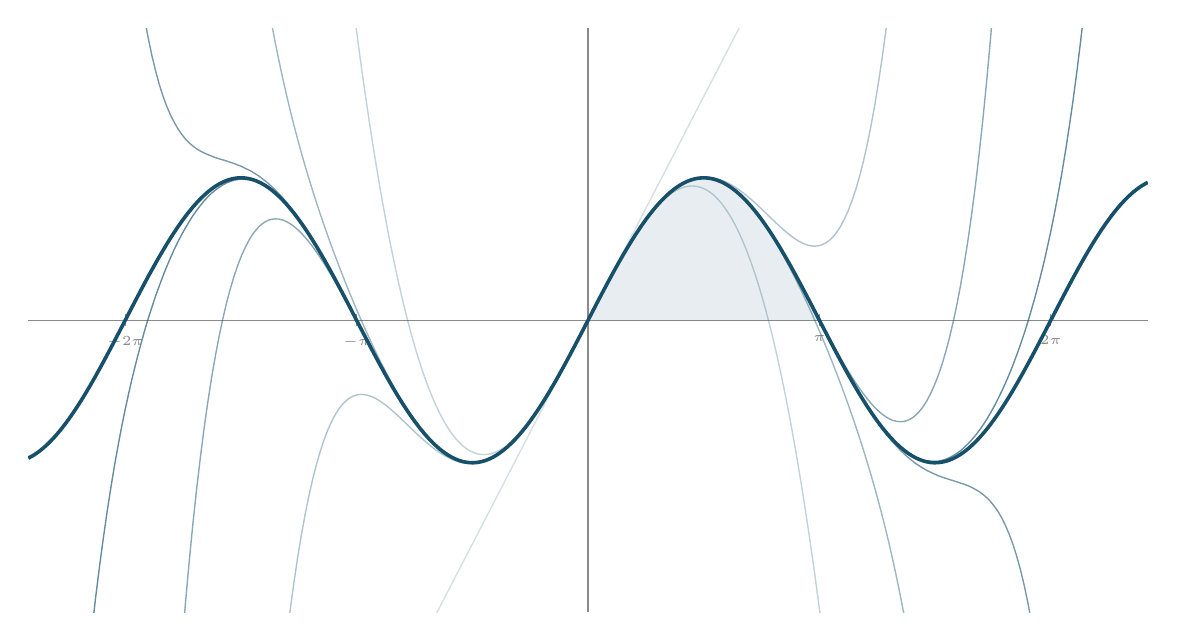
\begin{tikzpicture}
\begin{axis}[
  width=15.8cm, height=9.0cm,
  axis lines=middle,
  axis line style={soft, line width=0.4pt, -},
  xmin=-7.6, xmax=7.6, ymin=-2.05, ymax=2.05,
  domain=-7.6:7.6, samples=300,
  restrict y to domain=-2.3:2.3,
  xtick={-6.2832, -3.1416, 3.1416, 6.2832},
  xticklabels={$-2\pi$, $-\pi$, $\pi$, $2\pi$},
  ytick=\empty,
  tick label style={font=\tiny, color=soft},
  tick style={soft, line width=0.3pt},
  clip=true,
]
  \addplot[draw=none, domain=0:3.1416, name path=hump] {sin(deg(x))};
  \path[name path=base] (axis cs:0,0) -- (axis cs:3.1416,0);
  \addplot[accent, opacity=0.10] fill between[of=hump and base];

  \addplot[accent, opacity=0.18, line width=0.5pt] {x};
  \addplot[accent, opacity=0.26, line width=0.5pt] {x - x^3/6};
  \addplot[accent, opacity=0.34, line width=0.5pt] {x - x^3/6 + x^5/120};
  \addplot[accent, opacity=0.42, line width=0.5pt] {x - x^3/6 + x^5/120 - x^7/5040};
  \addplot[accent, opacity=0.50, line width=0.5pt]
     {x - x^3/6 + x^5/120 - x^7/5040 + x^9/362880};
  \addplot[accent, opacity=0.58, line width=0.5pt]
     {x - x^3/6 + x^5/120 - x^7/5040 + x^9/362880 - x^11/39916800};
  \addplot[accent, opacity=0.66, line width=0.5pt]
     {x - x^3/6 + x^5/120 - x^7/5040 + x^9/362880 - x^11/39916800 + x^13/6227020800};

  \addplot[accent, line width=1.3pt] {sin(deg(x))};
\end{axis}
\end{tikzpicture}}


\begin{document}

\includepdf[pages={1,2},pagecommand={\thispagestyle{empty}}]{澄潇宇大观题库-多元积分·无空版-封皮.pdf}

\pagenumbering{roman}
\setcounter{tocdepth}{1}
\tableofcontents
\clearpage
\pagenumbering{arabic}

\bookchapter{第一章 空间解析几何}{113}{ch01:chap}
\par\addvspace{2.4ex}\noindent
\begin{minipage}{\linewidth}
\qhead{1}{1.1}{向量计算}{ch01:sec:1.1}

% ---- item_id=e0a6a6b00183 seq=1.1-001 ----
\begin{q}{1.1-001}{1995数一}{ch01:q:e0a6a6b00183}
设 $(\mathbf{a}\times\mathbf{b})\cdot\mathbf{c}=2$，则 $[(\mathbf{a}+\mathbf{b})\times(\mathbf{b}+\mathbf{c})]\cdot(\mathbf{c}+\mathbf{a})=\underline{\hspace{4em}}$
\end{q}
\end{minipage}
\markboth{1.1\quad 向量计算}{1.1\quad 向量计算}


% ---- item_id=6d50cbd015f3 seq=1.1-002 ----
\begin{q}{1.1-002}{880第四章基础填空1}{ch01:q:6d50cbd015f3}
设向量 $a=(-1,3,0), b=(3,1,0), |c|=r$(常数). 当 $c$ 满足 $a=b\times c$ 时, $r$ 的最小值为 \underline{\hspace{4em}} .
\end{q}

% ---- item_id=7c0239494ee8 seq=1.1-003 ----
\begin{q}{1.1-003}{880第四章基础填空2}{ch01:q:7c0239494ee8}
设向量 $a=(2,-3,1),b=(1,-2,3),c=(2,1,2)$，向量 $r$ 满足 $r\perp a,r\perp b,\mathrm{Prj}_{c}r=14$，则 $r=\underline{\hspace{4em}}$.
\end{q}

% ---- item_id=4ed3597e1bf4 seq=1.1-004 ----
\begin{q}{1.1-004}{880第四章基础选择1}{ch01:q:4ed3597e1bf4}
(1) 设向量 $a=(1,2,1),b=(-1,0,2),c=(0,k,-3)$ 共面，则 $k=(\quad)$．
\begin{opts}{0.235}
\opt{A}{$1$}\hfill\opt{B}{$2$}\hfill\opt{C}{$-1$}\hfill\opt{D}{$-2$}
\end{opts}
\end{q}

% ---- item_id=351c298870a7 seq=1.1-005 ----
\begin{q}{1.1-005}{880第四章基础填空11}{ch01:q:351c298870a7}
设 $\alpha$ 与 $\beta$ 均为单位向量，其夹角为 $\frac{\pi}{6}$，则以 $\alpha+2\beta$ 与 $3\alpha+\beta$ 为邻边的平行四边形的面积为 $\underline{\hspace{4em}}$．
\end{q}

% ---- item_id=2d0194f9e3d7 seq=1.1-006 ----
\begin{q}{1.1-006}{880第四章基础填空12}{ch01:q:2d0194f9e3d7}
设 $\alpha$ 与 $\beta$ 是非零常向量，$|\beta|=2$（$|\beta|$ 表示 $\beta$ 的模），$\alpha$ 与 $\beta$ 之间的夹角为 $\frac{\pi}{3}$，求 $\displaystyle \lim\limits_{x\to 0}\frac{|\alpha+x\beta|-|\alpha|}{x}=$
\end{q}

% ---- item_id=5e228db2d0e8 seq=1.1-007 ----
\begin{q}{1.1-007}{900第四章A类4}{ch01:q:5e228db2d0e8}
若向量 $\boldsymbol{\alpha}=(1,0,0)$，$\boldsymbol{\beta}=(0,1,0)$，$\boldsymbol{\gamma}=(0,0,1)$，则 $[(\boldsymbol{\alpha}+\boldsymbol{\beta}+\boldsymbol{\gamma})\times(\boldsymbol{\alpha}+\boldsymbol{\beta})]\cdot\boldsymbol{\alpha}=\underline{\hspace{4em}}$。
\end{q}

% ---- item_id=c0a182647e09 seq=1.1-008 ----
\begin{q}{1.1-008}{660数一137}{ch01:q:c0a182647e09}
已知三个向量 $a,b,c$，其中 $c\perp a,c\perp b$，$a$ 与 $b$ 的夹角为 $\frac{\pi}{6}$，$|a|=6,|b|=|c|=3$，则 $(a\times b)\cdot c=\underline{\hspace{4em}}$
\end{q}

\par\addvspace{2.4ex}\noindent
\begin{minipage}{\linewidth}
\qhead{1}{1.2}{空间直线与平面}{ch01:sec:1.2}

\qhead{2}{1.2.1}{求直线方程}{ch01:sec:1.2.1}

\qhead{3}{1.2.1.1}{已知线面关系}{ch01:sec:1.2.1.1}

% ---- item_id=90dd7792133f seq=1.2.1.1-001 ----
\begin{q}{1.2.1.1-001}{880第四章基础解答5}{ch01:q:90dd7792133f}
求过点 $(-1,2,3)$，垂直于直线 $\frac{x}{4}=\frac{y}{5}=\frac{z}{6}$ 且平行于平面 $7x+8y+9z+10=0$ 的直线方程.
\end{q}
\end{minipage}
\markboth{1.2.1.1\quad 已知线面关系}{1.2.1.1\quad 已知线面关系}


% ---- item_id=5c10d1bdeb0c seq=1.2.1.1-002 ----
\begin{q}{1.2.1.1-002}{660数一139}{ch01:q:5c10d1bdeb0c}
过点 $P(-1,0,4)$ 且与平面 $3x-4y+z+10=0$ 平行，又与直线 $L:\frac{x+1}{1}=\frac{y-3}{1}=\frac{z}{2}$ 相交的直线方程是 $\underline{\hspace{4em}}$．
\end{q}

\par\addvspace{2.4ex}\noindent
\begin{minipage}{\linewidth}
\qhead{3}{1.2.1.2}{公垂线}{ch01:sec:1.2.1.2}

% ---- item_id=b9fcfcbe4a10 seq=1.2.1.2-001 ----
\begin{q}{1.2.1.2-001}{880第四章基础解答6}{ch01:q:b9fcfcbe4a10}
求与直线 $L_1:x+2=3-y=z+1$ 和 $L_2:\frac{x+4}{2}=y=\frac{z-4}{3}$ 都垂直相交的直线方程.
\end{q}
\end{minipage}
\markboth{1.2.1.2\quad 公垂线}{1.2.1.2\quad 公垂线}


% ---- item_id=6a1a2ba39c32 seq=1.2.1.2-002 ----
\begin{q}{1.2.1.2-002}{880第四章基础解答7}{ch01:q:6a1a2ba39c32}
求直线 $L_1:\frac{x-3}{2}=y=\frac{z-1}{0}$ 与 $L_2:\frac{x+1}{1}=\frac{y-2}{0}=z$ 的公垂线方程.
\end{q}

\par\addvspace{2.4ex}\noindent
\begin{minipage}{\linewidth}
\qhead{3}{1.2.1.3}{投影线}{ch01:sec:1.2.1.3}

% ---- item_id=8922c4948527 seq=1.2.1.3-001 ----
\begin{q}{1.2.1.3-001}{880第四章基础解答4}{ch01:q:8922c4948527}
求直线 $L:\frac{x+2}{3}=\frac{2-y}{1}=\frac{z+1}{2}$ 在平面 $\pi:2x+3y+3z-8=0$ 上的投影直线方程.
\end{q}
\end{minipage}
\markboth{1.2.1.3\quad 投影线}{1.2.1.3\quad 投影线}


% ---- item_id=5a893c936e10 seq=1.2.1.3-002 ----
\begin{q}{1.2.1.3-002}{880第四章基础填空7}{ch01:q:5a893c936e10}
直线 $L:\begin{cases} x+2y-3z=2,\\ 2x-y+z=3 \end{cases}$，在平面 $z=0$ 上的投影为 $\underline{\hspace{4em}}$，在平面 $z=1$ 上的投影为 $\underline{\hspace{4em}}$.
\end{q}

\par\addvspace{2.4ex}\noindent
\begin{minipage}{\linewidth}
\qhead{2}{1.2.2}{求平面方程}{ch01:sec:1.2.2}

\qhead{3}{1.2.2.1}{线线关系}{ch01:sec:1.2.2.1}

% ---- item_id=0fd76c2fb7a7 seq=1.2.2.1-001 ----
\begin{q}{1.2.2.1-001}{1987数一}{ch01:q:0fd76c2fb7a7}
与两直线 \[\begin{cases} x=1, \\ y=-1+t, \\ z=2+t \end{cases}\] 及 $\displaystyle \frac{x+1}{1}=\frac{y+2}{2}=\frac{z-1}{1}$ 都平行，且过原点的平面方程为 \underline{\hspace{4em}}
\end{q}
\end{minipage}
\markboth{1.2.2.1\quad 线线关系}{1.2.2.1\quad 线线关系}


% ---- item_id=917cd7a357c9 seq=1.2.2.1-002 ----
\begin{q}{1.2.2.1-002}{1991数一}{ch01:q:917cd7a357c9}
（3）已知两条直线 $L_1:\frac{x-1}{1}=\frac{y-2}{0}=\frac{z-3}{-1},L_2:\frac{x+2}{2}=\frac{y-1}{1}=\frac{z}{1}$，则过 $L_1$ 且平行于 $L_2$ 的平面方程是\underline{\hspace{4em}}
\end{q}

% ---- item_id=84137a6bcad6 seq=1.2.2.1-003 ----
\begin{q}{1.2.2.1-003}{900第四章A类6}{ch01:q:84137a6bcad6}
若直线 $l_1:\frac{x-4}{1}=\frac{y-2}{3}=\frac{z-1}{5}$ 在平面 $\pi$ 上的投影直线为 $l_2:\frac{x-4}{3}=\frac{y-2}{2}=\frac{z-1}{1}$，则平面 $\pi$ 的方程为 $\underline{\hspace{4em}}$.
\end{q}

% ---- item_id=9163b7653010 seq=1.2.2.1-004 ----
\begin{q}{1.2.2.1-004}{900第四章A类7}{ch01:q:9163b7653010}
10 与两直线 $\begin{cases} x=2,\\ y=t,\\ z=1+t \end{cases}$ 及 $\frac{x}{1}=\frac{y+1}{2}=\frac{z-1}{3}$ 都平行，且过原点的平面方程为 $\underline{\hspace{4em}}$.
\end{q}

% ---- item_id=c67ba335bb22 seq=1.2.2.1-005 ----
\begin{q}{1.2.2.1-005}{900第四章A类8}{ch01:q:c67ba335bb22}
11 已知两条直线的方程是
$\displaystyle L_1:\frac{x-1}{1}=\frac{y-2}{1}=\frac{z-1}{-1},\quad L_2:\frac{x+2}{2}=\frac{y-1}{1}=\frac{z}{1},$
则过 $L_1$ 且平行于 $L_2$ 的平面方程是 \underline{\hspace{4em}}.
\end{q}

\par\addvspace{2.4ex}\noindent
\begin{minipage}{\linewidth}
\qhead{3}{1.2.2.2}{点线关系}{ch01:sec:1.2.2.2}

% ---- item_id=f35c05ce13e6 seq=1.2.2.2-001 ----
\begin{q}{1.2.2.2-001}{1990数一}{ch01:q:f35c05ce13e6}
过点 $M(1,2,-1)$ 且与直线 \[\begin{cases} x=-t+2 \\ y=3t-4 \\ z=t-1 \end{cases}\] 垂直的平面方程是 \underline{\hspace{4em}}
\end{q}
\end{minipage}
\markboth{1.2.2.2\quad 点线关系}{1.2.2.2\quad 点线关系}


% ---- item_id=f2ac298199cb seq=1.2.2.2-002 ----
\begin{q}{1.2.2.2-002}{880第四章基础填空3}{ch01:q:f2ac298199cb}
过点 $(2,0,-3)$ 且与直线 $\begin{cases} x-2y+4z-7=0,\\ 3x+5y-2z+1=0 \end{cases}$ 垂直的平面方程为 $\underline{\hspace{4em}}$.
\end{q}

% ---- item_id=4bedabdabb68 seq=1.2.2.2-003 ----
\begin{q}{1.2.2.2-003}{880第四章基础填空8}{ch01:q:4bedabdabb68}
过点 $A(1,1,-1),B(-2,-2,2)$ 和 $C(1,-1,2)$ 三点的平面方程为 \underline{\hspace{4em}}.
\end{q}

\par\addvspace{2.4ex}\noindent
\begin{minipage}{\linewidth}
\qhead{3}{1.2.2.3}{平面束}{ch01:sec:1.2.2.3}

% ---- item_id=5ec9aa5b9008 seq=1.2.2.3-001 ----
\begin{q}{1.2.2.3-001}{880第四章基础解答2}{ch01:q:5ec9aa5b9008}
设平面 $\pi$ 与点 $P(1,2,1)$ 的距离为 $1$，且过直线 \[L:\begin{cases}3x-2y+2=0,\\ x-2y-z+6=0,\end{cases}\] 求平面 $\pi$ 的方程.
\end{q}
\end{minipage}
\markboth{1.2.2.3\quad 平面束}{1.2.2.3\quad 平面束}


% ---- item_id=9bcde0ba1deb seq=1.2.2.3-002 ----
\begin{q}{1.2.2.3-002}{880第四章基础解答3}{ch01:q:9bcde0ba1deb}
设平面 $\pi$ 过直线 $L:\begin{cases} x+5y+z=0, \\ x-z+4=0, \end{cases}$ 且与平面 $\pi_1:x-4y-8z+12=0$ 的夹角为 $45^\circ$，求平面 $\pi$ 的方程.
\end{q}

\par\addvspace{2.4ex}\noindent
\begin{minipage}{\linewidth}
\qhead{3}{1.2.2.4}{点面关系}{ch01:sec:1.2.2.4}

% ---- item_id=6c8305891950 seq=1.2.2.4-001 ----
\begin{q}{1.2.2.4-001}{1996数一}{ch01:q:6c8305891950}
设一平面经过原点及 $(6,-3,2)$，且与平面 $4x-y+2z=8$ 垂直，则此平面方程为 $\underline{\hspace{4em}}$
\end{q}
\end{minipage}
\markboth{1.2.2.4\quad 点面关系}{1.2.2.4\quad 点面关系}


\par\addvspace{2.4ex}\noindent
\begin{minipage}{\linewidth}
\qhead{3}{1.2.2.5}{面面关系}{ch01:sec:1.2.2.5}

% ---- item_id=de10b182a010 seq=1.2.2.5-001 ----
\begin{q}{1.2.2.5-001}{880第四章基础解答1}{ch01:q:de10b182a010}
求平行于平面 $x+y+z=9$ 且与球面 $x^2+y^2+z^2=4$ 相切的平面方程。
\end{q}
\end{minipage}
\markboth{1.2.2.5\quad 面面关系}{1.2.2.5\quad 面面关系}


\par\addvspace{2.4ex}\noindent
\begin{minipage}{\linewidth}
\qhead{3}{1.2.2.6}{面距关系}{ch01:sec:1.2.2.6}

% ---- item_id=f030f6142839 seq=1.2.2.6-001 ----
\begin{q}{1.2.2.6-001}{660数一136}{ch01:q:f030f6142839}
平行于平面 $5x-14y+2z+36=0$ 且距此平面距离为 $3$ 的平面方程为 $\underline{\hspace{4em}}$．
\end{q}
\end{minipage}
\markboth{1.2.2.6\quad 面距关系}{1.2.2.6\quad 面距关系}


\par\addvspace{2.4ex}\noindent
\begin{minipage}{\linewidth}
\qhead{2}{1.2.3}{求夹角}{ch01:sec:1.2.3}

% ---- item_id=c29b9607d5ab seq=1.2.3-001 ----
\begin{q}{1.2.3-001}{1993数一; 880第四章基础选择2}{ch01:q:c29b9607d5ab}
(3) 设有直线 $L_1:\frac{x-1}{1}=\frac{y-5}{-2}=\frac{z+8}{1}$ 与 $L_2:\begin{cases} x-y=6,\\ 2y+z=3, \end{cases}$ 则 $L_1$ 与 $L_2$ 的夹角为（\quad）
\begin{opts}{0.235}
\opt{A}{$\frac{\pi}{6}.$}\hfill\opt{B}{$\frac{\pi}{4}.$}\hfill\opt{C}{$\frac{\pi}{3}.$}\hfill\opt{D}{$\frac{\pi}{2}.$}
\end{opts}
\end{q}
\end{minipage}
\markboth{1.2.3\quad 求夹角}{1.2.3\quad 求夹角}


% ---- item_id=2ca5e1ed5a7a seq=1.2.3-002 ----
\begin{q}{1.2.3-002}{900第四章A类1}{ch01:q:2ca5e1ed5a7a}
已知直线 $l_1$ 过点 $(1,2,3)$ 和 $(9,4,1)$，则直线 $l_1$ 与直线 $l_2$：$\begin{cases} x+2y+3z=1,\\ 9x+4y+z=1 \end{cases}$ 的夹角为（  ）
\begin{opts}{0.235}
\opt{A}{$0.$}\hfill\opt{B}{$\frac{\pi}{6}.$}\hfill\opt{C}{$\frac{\pi}{3}.$}\hfill\opt{D}{$\frac{\pi}{2}.$}
\end{opts}
\end{q}

% ---- item_id=fc3d0c0ae542 seq=1.2.3-003 ----
\begin{q}{1.2.3-003}{660数一341}{ch01:q:fc3d0c0ae542}
341 直线 $L:\frac{x-2}{2}=\frac{y-1}{1}=\frac{z-3}{1}$ 与平面 $\Pi:x-y+2z+4=0$ 的夹角为
\begin{opts}{0.235}
\opt{A}{$\pi$.}\hfill\opt{B}{$\frac{\pi}{3}$.}\hfill\opt{C}{$\frac{\pi}{6}$.}\hfill\opt{D}{$\frac{\pi}{2}$.}
\end{opts}
\end{q}

\par\addvspace{2.4ex}\noindent
\begin{minipage}{\linewidth}
\qhead{2}{1.2.4}{求距离}{ch01:sec:1.2.4}

% ---- item_id=6e2e4e0c3b10 seq=1.2.4-001 ----
\begin{q}{1.2.4-001}{2006数一}{ch01:q:6e2e4e0c3b10}
点 $(2,1,0)$ 到平面 $3x+4y+5z=0$ 的距离 $d = \underline{\hspace{4em}}$
\end{q}
\end{minipage}
\markboth{1.2.4\quad 求距离}{1.2.4\quad 求距离}


% ---- item_id=288aa8438128 seq=1.2.4-002 ----
\begin{q}{1.2.4-002}{880第四章基础填空4}{ch01:q:288aa8438128}
点 $P(1,-1,2)$ 到平面 $\pi: 2x-y+5z-12=0$ 的距离 $d=\underline{\hspace{4em}}$。
\end{q}

% ---- item_id=90d1665c2e23 seq=1.2.4-003 ----
\begin{q}{1.2.4-003}{880第四章基础填空5}{ch01:q:90d1665c2e23}
点 $P(1,-1,0)$ 到直线 $L:\frac{x}{3}=\frac{y}{3}=\frac{z+1}{2}$ 的距离 $d=\underline{\hspace{4em}}$.
\end{q}

% ---- item_id=61bbfba088f3 seq=1.2.4-004 ----
\begin{q}{1.2.4-004}{660数一138}{ch01:q:61bbfba088f3}
点 $M(3,2,6)$ 到直线 $\frac{x}{1}=\frac{y+7}{2}=\frac{z-3}{-1}$ 的距离为 \underline{\hspace{4em}}.
\end{q}

% ---- item_id=f00c77c8a10f seq=1.2.4-005 ----
\begin{q}{1.2.4-005}{880第四章基础填空6}{ch01:q:f00c77c8a10f}
直线 $L_1:\begin{cases} x-1=0, \\ y=z \end{cases}$ 与 $L_2:\begin{cases} x+2y=0, \\ z+2=0 \end{cases}$ 之间的距离 $d=\underline{\hspace{4em}}$ .
\end{q}

% ---- item_id=4d9b6c54c6b5 seq=1.2.4-006 ----
\begin{q}{1.2.4-006}{900第四章A类5}{ch01:q:4d9b6c54c6b5}
点 $(1,2,0)$ 到平面 $3x+4y+5z=0$ 的距离 $d=\underline{\hspace{4em}}$.
\end{q}

% ---- item_id=b27d25eb12e6 seq=1.2.4-007 ----
\begin{q}{1.2.4-007}{1000第17章强化2}{ch01:q:b27d25eb12e6}
求曲面 $4z=3x^2-2xy+3y^2$ 上的点到平面 $x+y-4z=1$ 的最短距离.
\end{q}

\par\addvspace{2.4ex}\noindent
\begin{minipage}{\linewidth}
\qhead{2}{1.2.5}{直线平面的位置关系}{ch01:sec:1.2.5}

% ---- item_id=54aed8c6af29 seq=1.2.5-001 ----
\begin{q}{1.2.5-001}{1995数一; 1000第17章基础2; 660数一342; 880第四章基础选择3}{ch01:q:54aed8c6af29}
（1）设有直线 $L$：\[\begin{cases} x+3y+2z+1=0,\\ 2x-y-10z+3=0 \end{cases}\] 及平面 $\pi:4x-2y+z-2=0$，则直线 $L$（\quad）
\begin{opts}{0.235}
\opt{A}{平行于 $\pi$．}\hfill\opt{B}{在 $\pi$ 上．}\hfill\opt{C}{垂直于 $\pi$．}\hfill\opt{D}{与 $\pi$ 斜交．}
\end{opts}
\end{q}
\end{minipage}
\markboth{1.2.5\quad 直线平面的位置关系}{1.2.5\quad 直线平面的位置关系}


% ---- item_id=ad9ac7921593 seq=1.2.5-002 ----
\begin{q}{1.2.5-002}{900第四章A类2}{ch01:q:ad9ac7921593}
已知平面 $\pi$ 过原点且直线 $l:\frac{x-3}{1}=\frac{y+2}{2}=\frac{z-6}{3}$ 在平面 $\pi$ 上，则下列直线在平面 $\pi$ 上的是（ ）
\begin{opts}{0.48}
\opt{A}{$l_1:\frac{x+1}{1}=\frac{y-6}{-6}=\frac{z}{-1}$.}\hfill\opt{B}{$l_2:\frac{x-2}{2}=\frac{y+4}{-3}=\frac{z-3}{3}$.}\\[0.3ex]
\opt{C}{$l_3:\frac{x-1}{2}=\frac{y-1}{-4}=\frac{z-3}{3}$.}\hfill\opt{D}{$l_4:\frac{x+1}{1}=\frac{y-6}{2}=\frac{z}{3}$.}
\end{opts}
\end{q}

\par\addvspace{2.4ex}\noindent
\begin{minipage}{\linewidth}
\qhead{1}{1.3}{空间曲线与曲面}{ch01:sec:1.3}

\qhead{2}{1.3.1}{空间曲线}{ch01:sec:1.3.1}

\qhead{3}{1.3.1.1}{求曲线方程}{ch01:sec:1.3.1.1}

% ---- item_id=3af2d1af57fd seq=1.3.1.1-001 ----
\begin{q}{1.3.1.1-001}{880第四章基础填空10}{ch01:q:3af2d1af57fd}
曲线 $\begin{cases} z=2x^2+3y^2, \\ z=12-x^2-3y^2 \end{cases}$ 在 $xOy$ 面上的投影曲线方程为 $\underline{\hspace{4em}}$.
\end{q}
\end{minipage}
\markboth{1.3.1.1\quad 求曲线方程}{1.3.1.1\quad 求曲线方程}


\par\addvspace{2.4ex}\noindent
\begin{minipage}{\linewidth}
\qhead{3}{1.3.1.2}{切线与法平面}{ch01:sec:1.3.1.2}

% ---- item_id=e8daefd3df6f seq=1.3.1.2-001 ----
\begin{q}{1.3.1.2-001}{1992数一}{ch01:q:e8daefd3df6f}
（3）在曲线 $x=t,y=-t^2,z=t^3$ 的所有切线中,与平面 $x+2y+z=4$ 平行的切线（ ）
\begin{opts}{0.235}
\opt{A}{只有 1 条.}\hfill\opt{B}{只有 2 条.}\hfill\opt{C}{至少有 3 条.}\hfill\opt{D}{不存在.}
\end{opts}
\end{q}
\end{minipage}
\markboth{1.3.1.2\quad 切线与法平面}{1.3.1.2\quad 切线与法平面}


% ---- item_id=149ea2168dbf seq=1.3.1.2-002 ----
\begin{q}{1.3.1.2-002}{2001数一}{ch01:q:149ea2168dbf}
（2）设函数 $f(x,y)$ 在点 $(0,0)$ 附近有定义，且 $f_x'(0,0)=3$，$f_y'(0,0)=1$，则（\quad）
\begin{opts}{0.97}
\opt{A}{$\left.dz\right|_{(0,0)}=3dx+dy$.}\\[0.3ex]
\opt{B}{曲面 $z=f(x,y)$ 在点 $(0,0,f(0,0))$ 的法向量为 $(3,1,1)$.}\\[0.3ex]
\opt{C}{曲线 $\begin{cases} z=f(x,y),\\ y=0 \end{cases}$ 在点 $(0,0,f(0,0))$ 的切向量为 $(1,0,3)$.}\\[0.3ex]
\opt{D}{曲线 $\begin{cases} z=f(x,y),\\ y=0 \end{cases}$ 在点 $(0,0,f(0,0))$ 的切向量为 $(3,0,1)$.}
\end{opts}
\end{q}

% ---- item_id=06730c0f0539 seq=1.3.1.2-003 ----
\begin{q}{1.3.1.2-003}{1000第17章强化3}{ch01:q:06730c0f0539}
空间曲线 $L$: \[ \begin{cases} y^2=z, \\ x=2(y-1) \end{cases} \] 在 $y=1$ 处的切线方程为 \underline{\hspace{4em}}。
\end{q}

% ---- item_id=31792a89007c seq=1.3.1.2-004 ----
\begin{q}{1.3.1.2-004}{660数一343}{ch01:q:31792a89007c}
曲线 \[\begin{cases} x^2+y^2+z^2=2 \\ x+y+z=0 \end{cases}\] 在点 $(1,-1,0)$ 处的切线方程为
\begin{opts}{0.48}
\opt{A}{$\frac{x-1}{2}=y+1=z.$}\hfill\opt{B}{$\frac{x-1}{2}=\frac{y+1}{2}=\frac{z}{3}.$}\\[0.3ex]
\opt{C}{$\frac{x-1}{-1}=\frac{y+1}{-1}=\frac{z}{1}.$}\hfill\opt{D}{$x-1=y+1=-\frac{z}{2}.$}
\end{opts}
\end{q}

% ---- item_id=dfddb7049086 seq=1.3.1.2-005 ----
\begin{q}{1.3.1.2-005}{1000第17章强化4}{ch01:q:dfddb7049086}
曲线 $\begin{cases} x^2+2y^2+3z^2=6, \\ x+y+z=3 \end{cases}$ 在点 $(1,1,1)$ 处的切线方程为 $\underline{\hspace{4em}}$．
\end{q}

% ---- item_id=1b611462499d seq=1.3.1.2-006 ----
\begin{q}{1.3.1.2-006}{1000第17章强化6}{ch01:q:1b611462499d}
设函数 $z=f(x,y)$ 在点 $(0,0)$ 附近有定义，且 $f'_x(0,0)=3$，则曲线
\[\begin{cases}
z=f(x,y),\\
y=0
\end{cases}\]
在点 $(0,0,f(0,0))$ 处的法平面方程为 $\underline{\hspace{4em}}$.
\end{q}

\par\addvspace{2.4ex}\noindent
\begin{minipage}{\linewidth}
\qhead{2}{1.3.2}{空间曲面}{ch01:sec:1.3.2}

\qhead{3}{1.3.2.1}{旋转曲面方程}{ch01:sec:1.3.2.1}

% ---- item_id=546d26dfe9d9 seq=1.3.2.1-001 ----
\begin{q}{1.3.2.1-001}{1998数一}{ch01:q:546d26dfe9d9}
求直线 $l:\frac{x-1}{1}=\frac{y}{1}=\frac{z-1}{-1}$ 在平面 $\pi:x-y+2z-1=0$ 上的投影直线 $l_0$ 的方程，并求 $l_0$ 绕 $y$ 轴旋转一周所成曲面的方程.
\end{q}
\end{minipage}
\markboth{1.3.2.1\quad 旋转曲面方程}{1.3.2.1\quad 旋转曲面方程}


% ---- item_id=028971b57920 seq=1.3.2.1-002 ----
\begin{q}{1.3.2.1-002}{880第四章基础填空9}{ch01:q:028971b57920}
曲线 $\begin{cases} x^2+2z^2=4, \\ y=0 \end{cases}$ 绕 $z$ 轴旋转一周所得的旋转曲面方程为 \underline{\hspace{4em}}.
\end{q}

% ---- item_id=87c152010633 seq=1.3.2.1-003 ----
\begin{q}{1.3.2.1-003}{880第四章基础解答8}{ch01:q:87c152010633}
求直线 $\frac{x-1}{0}=\frac{y}{1}=\frac{z-1}{2}$ 绕 $z$ 轴旋转一周所得的旋转曲面方程.
\end{q}

% ---- item_id=033407f4aec1 seq=1.3.2.1-004 ----
\begin{q}{1.3.2.1-004}{880第四章基础解答9}{ch01:q:033407f4aec1}
求直线 $L:\frac{x-1}{3}=\frac{y-2}{4}=\frac{z+1}{1}$ 绕直线 $\begin{cases} x=2, \\ y=3 \end{cases}$ 旋转一周所得的曲面方程.
\end{q}

% ---- item_id=9c2eaef66731 seq=1.3.2.1-005 ----
\begin{q}{1.3.2.1-005}{900第四章A类9}{ch01:q:9c2eaef66731}
12 求直线 $l:\frac{x}{2}=\frac{y-1}{2}=\frac{z-1}{-1}$ 在平面 $\pi:x-y+2z-1=0$ 上的投影直线 $l_0$ 的方程，并求 $l_0$ 绕 $y$ 轴旋转一周所成曲面的方程.
\end{q}

% ---- item_id=0eab31168444 seq=1.3.2.1-006 ----
\begin{q}{1.3.2.1-006}{900第四章A类3}{ch01:q:0eab31168444}
6 直线 $l:\begin{cases}3x+y+2z-2=0,\\x+2y-z-\frac{3}{2}=0\end{cases}$ 绕 $z$ 轴旋转一周的曲面记为 $\Sigma$，则下列说法中，正确的是（ ）
\begin{opts}{0.48}
\opt{A}{直线 $x-\frac{1}{2}=\frac{1}{2}-y=-z$ 在曲面 $\Sigma$ 上.}\hfill\opt{B}{直线 $\begin{cases}y=\sqrt{2}z,\\x=0\end{cases}$ 在 $\Sigma$ 上.}\\[0.3ex]
\opt{C}{曲面 $\Sigma$ 的方程为 $-x^2+y^2+2z^2=\frac{1}{2}$.}\hfill\opt{D}{曲面 $\Sigma$ 的方程为 $x^2-y^2+2z^2=\frac{1}{2}$.}
\end{opts}
\end{q}

% ---- item_id=72f7e6a3d850 seq=1.3.2.1-007 ----
\begin{q}{1.3.2.1-007}{2009数一}{ch01:q:72f7e6a3d850}
椭球面 $S_1$ 是椭圆 $\frac{x^2}{4}+\frac{y^2}{3}=1$ 绕 $x$ 轴旋转而成，圆锥面 $S_2$ 是由过点 $(4,0)$ 且与椭圆 $\frac{x^2}{4}+\frac{y^2}{3}=1$ 相切的直线绕 $x$ 轴旋转而成。

（I）求 $S_1$ 及 $S_2$ 的方程；

（II）求 $S_1$ 与 $S_2$ 之间的立体的体积。
\end{q}

\par\addvspace{2.4ex}\noindent
\begin{minipage}{\linewidth}
\qhead{3}{1.3.2.2}{切平面与法线}{ch01:sec:1.3.2.2}

% ---- item_id=88028149f8a4 seq=1.3.2.2-001 ----
\begin{q}{1.3.2.2-001}{1994数一}{ch01:q:88028149f8a4}
曲面 $z-\mathrm{e}^z+2xy=3$ 在点 $(1,2,0)$ 处的切平面方程为 $\underline{\hspace{4em}}$
\end{q}
\end{minipage}
\markboth{1.3.2.2\quad 切平面与法线}{1.3.2.2\quad 切平面与法线}


% ---- item_id=c4aa6c6a2b33 seq=1.3.2.2-002 ----
\begin{q}{1.3.2.2-002}{1000第17章强化7}{ch01:q:c4aa6c6a2b33}
曲面 $e^z-xz+y=3$ 在点 $(1,2,0)$ 处的切平面方程为 \underline{\hspace{4em}}.
\end{q}

% ---- item_id=fe764c1fc1cc seq=1.3.2.2-003 ----
\begin{q}{1.3.2.2-003}{2003数一}{ch01:q:fe764c1fc1cc}
曲面 $z=x^{2}+y^{2}$ 与平面 $2x+4y-z=0$ 平行的切平面的方程是 $\underline{\hspace{4em}}$
\end{q}

% ---- item_id=e154baf95b1f seq=1.3.2.2-004 ----
\begin{q}{1.3.2.2-004}{2013数一}{ch01:q:e154baf95b1f}
(2) 曲面 $x^2+\cos(xy)+yz+x=0$ 在点 $(0,1,-1)$ 处的切平面方程为（ ）
\begin{opts}{0.235}
\opt{A}{$x-y+z=-2$}\hfill\opt{B}{$x+y+z=0$}\hfill\opt{C}{$x-2y+z=-3$}\hfill\opt{D}{$x-y-z=0$}
\end{opts}
\end{q}

% ---- item_id=2d57d3095689 seq=1.3.2.2-005 ----
\begin{q}{1.3.2.2-005}{2014数一}{ch01:q:2d57d3095689}
曲面 $z=x^2(1-\sin y)+y^2(1-\sin x)$ 在点 $(1,0,1)$ 处的切平面方程为 \underline{\hspace{4em}}
\end{q}

% ---- item_id=4240020772f4 seq=1.3.2.2-006 ----
\begin{q}{1.3.2.2-006}{2018数一}{ch01:q:4240020772f4}
(2) 过点 $(1,0,0),(0,1,0)$，且与曲面 $z=x^2+y^2$ 相切的平面为（　　）
\begin{opts}{0.48}
\opt{A}{$z=0$ 与 $x+y-z=1$.}\hfill\opt{B}{$z=0$ 与 $2x+2y-z=2$.}\\[0.3ex]
\opt{C}{$x=y$ 与 $x+y-z=1$.}\hfill\opt{D}{$x=y$ 与 $2x+2y-z=2$.}
\end{opts}
\end{q}

% ---- item_id=264311e53543 seq=1.3.2.2-007 ----
\begin{q}{1.3.2.2-007}{1000第17章基础4}{ch01:q:264311e53543}
过点 $(1,0,1)$ 与点 $(0,1,1)$ 且与曲面 $z=1+x^2+y^2$ 相切的平面为 $\underline{\hspace{4em}}$。
\end{q}

% ---- item_id=c712ebc19158 seq=1.3.2.2-008 ----
\begin{q}{1.3.2.2-008}{2023数一}{ch01:q:c712ebc19158}
曲面 $z=x+2y+\ln(1+x^2+y^2)$ 在点 $(0,0,0)$ 处的切平面方程为 $\underline{\hspace{4em}}$
\end{q}

% ---- item_id=59928cafc9a2 seq=1.3.2.2-009 ----
\begin{q}{1.3.2.2-009}{1000第17章基础3}{ch01:q:59928cafc9a2}
曲面 $z=4-x^2-y^2$ 在点 $P(1,1,2)$ 处的切平面方程为 $\underline{\hspace{4em}}$.
\end{q}

% ---- item_id=44925a4f17cc seq=1.3.2.2-010 ----
\begin{q}{1.3.2.2-010}{1000第17章基础5}{ch01:q:44925a4f17cc}
已知曲面 $z=f(x,y)$ 由方程 $z-x\ln(1+z^2)+e^y=0$ 所确定，则该曲面在点 $(0,0,-1)$ 处的切平面方程为 $\underline{\hspace{4em}}$.
\end{q}

% ---- item_id=f9216f95b828 seq=1.3.2.2-011 ----
\begin{q}{1.3.2.2-011}{2024数一}{ch01:q:f9216f95b828}
已知函数 $f(x, y) = x^3 + y^3 - (x+y)^2 + 3$，设 $T$ 是曲面 $z = f(x, y)$ 在点 $(1, 1, 1)$ 处的切平面，$D$ 为 $T$ 与坐标平面所围有界区域在 $xOy$ 平面上的投影.

（\rn{I}）求 $T$ 的方程；

（\rn{II}）求 $f(x, y)$ 在 $D$ 上的最大值和最小值.
\end{q}

% ---- item_id=2df6a20c3fe0 seq=1.3.2.2-012 ----
\begin{q}{1.3.2.2-012}{1997数一}{ch01:q:2df6a20c3fe0}
（1）设直线 $l:\begin{cases}x+y+b=0,\\ x+ay-z-3=0\end{cases}$ 在平面 $\Pi$ 上，而平面 $\Pi$ 与曲面 $z=x^2+y^2$ 相切于点 $(1,-2,5)$，求 $a,b$ 的值
\end{q}

% ---- item_id=ecbbb3d2bf16 seq=1.3.2.2-013 ----
\begin{q}{1.3.2.2-013}{1989数一}{ch01:q:ecbbb3d2bf16}
(2) 已知曲面 $z=4-x^2-y^2$ 上点 $P$ 处的切平面平行于平面 $2x+2y+z-1=0$，则点 $P$ 的坐标是（ ）
\begin{opts}{0.235}
\opt{A}{$(1,-1,2)$.}\hfill\opt{B}{$(-1,1,2)$.}\hfill\opt{C}{$(1,1,2)$.}\hfill\opt{D}{$(-1,-1,2)$.}
\end{opts}
\end{q}

% ---- item_id=1b479ade0a2b seq=1.3.2.2-014 ----
\begin{q}{1.3.2.2-014}{1993数一}{ch01:q:1b479ade0a2b}
(2) 由曲线 \[\begin{cases}3x^2+2y^2=12,\\ z=0\end{cases}\] 绕 $y$ 轴旋转一周得到的旋转面在点 $(0,\sqrt{3},\sqrt{2})$ 处的指向外侧的单位法向量为 \underline{\hspace{4em}}
\end{q}

% ---- item_id=5422d937fad9 seq=1.3.2.2-015 ----
\begin{q}{1.3.2.2-015}{2000数一}{ch01:q:5422d937fad9}
曲面 $x^2+2y^2+3z^2=21$ 在点 $(1,-2,2)$ 的法线方程为 $\underline{\hspace{4em}}$
\end{q}

\par\addvspace{2.4ex}\noindent
\begin{minipage}{\linewidth}
\qhead{3}{1.3.2.3}{其他}{ch01:sec:1.3.2.3}

% ---- item_id=0ef652f7fae6 seq=1.3.2.3-001 ----
\begin{q}{1.3.2.3-001}{1000第17章基础7}{ch01:q:0ef652f7fae6}
求以 $M_0(1,1,1)$ 为顶点，以曲线 $C$（$C$ 是平面 $z=0$ 上 $y^2=x$ 被 $x=1$ 截下的有限部分）为准线的锥面方程.
\end{q}
\end{minipage}
\markboth{1.3.2.3\quad 其他}{1.3.2.3\quad 其他}


% ---- item_id=2ea8bfd6e307 seq=1.3.2.3-002 ----
\begin{q}{1.3.2.3-002}{660数一135}{ch01:q:2ea8bfd6e307}
平面 $\Pi:x-2y+2z+9=0$ 与以点 $M_0(2,0,-1)$ 为球心的球面相切，则该球面的方程是 \underline{\hspace{4em}}.
\end{q}

% ---- item_id=cd06c9598435 seq=1.3.2.3-003 ----
\begin{q}{1.3.2.3-003}{660数一344}{ch01:q:cd06c9598435}
344 曲线 $L$：\[\begin{cases}\frac{x^2}{16}+\frac{y^2}{4}-\frac{z^2}{5}=1,\\ x-2z+3=0\end{cases}\] 在 $xOy$ 面上的投影柱面方程是
\begin{opts}{0.48}
\opt{A}{$x^2+20y^2-24x-116=0.$}\hfill\opt{B}{$4y^2+4z^2-12z-7=0.$}\\[0.3ex]
\opt{C}{$\begin{cases}x^2+20y^2-24x-116=0,\\ z=0.\end{cases}$}\hfill\opt{D}{$\begin{cases}4y^2+4z^2-12z-7=0,\\ x=0.\end{cases}$}
\end{opts}
\end{q}

% ---- item_id=faded2c46c7d seq=1.3.2.3-004 ----
\begin{q}{1.3.2.3-004}{880第四章拓展}{ch01:q:faded2c46c7d}
求满足下列条件的动点的轨迹方程，并说明它们分别表示什么曲面．
（I）动点到坐标原点的距离等于它到平面 $z=4$ 的距离；
（II）动点到坐标原点的距离等于它到点 $(2,3,4)$ 的距离的一半；
（III）动点到点 $(0,0,5)$ 的距离等于它到 $x$ 轴的距离；
（IV）动点到 $x$ 轴的距离等于它到 $yOz$ 面的距离的两倍．
\end{q}

\par\addvspace{2.4ex}\noindent
\begin{minipage}{\linewidth}
\qhead{1}{1.4}{场论}{ch01:sec:1.4}

\qhead{2}{1.4.1}{方向导数}{ch01:sec:1.4.1}

\qhead{3}{1.4.1.1}{直接计算方向导数}{ch01:sec:1.4.1.1}

% ---- item_id=ddc72e8ed944 seq=1.4.1.1-001 ----
\begin{q}{1.4.1.1-001}{1991数一}{ch01:q:ddc72e8ed944}
(2) 设 $n$ 是曲面 $2x^2+3y^2+z^2=6$ 在点 $P(1,1,1)$ 处的指向外侧的法向量，求函数 $u=\frac{\sqrt{6x^2+8y^2}}{z}$ 在点 $P$ 处沿方向 $n$ 的方向导数.
\end{q}
\end{minipage}
\markboth{1.4.1.1\quad 直接计算方向导数}{1.4.1.1\quad 直接计算方向导数}


% ---- item_id=267f55726955 seq=1.4.1.1-002 ----
\begin{q}{1.4.1.1-002}{1996数一}{ch01:q:267f55726955}
函数 $u=\ln(x+\sqrt{y^2+z^2})$ 在点 $A(1,0,1)$ 处沿点 $A$ 指向点 $B(3,-2,2)$ 方向的方向导数为 $\underline{\hspace{4em}}$.
\end{q}

% ---- item_id=1f1b7855f8bc seq=1.4.1.1-003 ----
\begin{q}{1.4.1.1-003}{2005数一}{ch01:q:1f1b7855f8bc}
设函数 $u(x,y,z)=1+\frac{x^2}{6}+\frac{y^2}{12}+\frac{z^2}{18}$，单位向量 $\mathbf{n}=\frac{1}{\sqrt{3}}(1,1,1)$，则 $\left.\frac{\partial u}{\partial \mathbf{n}}\right|_{(1,2,3)} = \underline{\hspace{4em}}$
\end{q}

% ---- item_id=6d3aaf600bda seq=1.4.1.1-004 ----
\begin{q}{1.4.1.1-004}{2017数一}{ch01:q:6d3aaf600bda}
（3）函数 $f(x,y,z)=x^2y+z^2$ 在点 $(1,2,0)$ 处沿向量 $\mathbf{n}=(1,2,2)$ 的方向导数为（ ）
\begin{opts}{0.235}
\opt{A}{$12.$}\hfill\opt{B}{$6.$}\hfill\opt{C}{$4.$}\hfill\opt{D}{$2.$}
\end{opts}
\end{q}

% ---- item_id=6858e38ba5bc seq=1.4.1.1-005 ----
\begin{q}{1.4.1.1-005}{2025数一}{ch01:q:6858e38ba5bc}
已知函数 $v(x,y,z)=xy^2z^3$，向量 $\vec{n}=(2,2,-1)$，则 $\left.\frac{\partial v}{\partial \vec{n}}\right|_{(1,1,1)}=\underline{\hspace{4em}}$。
\end{q}

% ---- item_id=803519ac016d seq=1.4.1.1-006 ----
\begin{q}{1.4.1.1-006}{1000第17章基础6}{ch01:q:803519ac016d}
设 $z=\ln\left(\mathrm{e}^{-y}+\dfrac{y^2}{x}\right)$ 在点 $(1,1)$ 处沿 $l=(1,0)$ 的方向导数为 \underline{\hspace{4em}}．
\end{q}

% ---- item_id=1d74aa249fa2 seq=1.4.1.1-007 ----
\begin{q}{1.4.1.1-007}{1000第17章基础8}{ch01:q:1d74aa249fa2}
设函数 $f(x,y)=\begin{cases}\dfrac{x^2|y|}{x^2+y^2}, & (x,y)\neq(0,0),\\ 0, & (x,y)=(0,0),\end{cases}$，则 $f(x,y)$ 在点 $(0,0)$ 处沿 $l=(1,1)$ 的方向导数是 \underline{\hspace{4em}}．
\end{q}

% ---- item_id=e1271ff139d7 seq=1.4.1.1-008 ----
\begin{q}{1.4.1.1-008}{660数一360}{ch01:q:e1271ff139d7}
函数 $f(x,y,z)=x^2+y^2+z^2$ 在点 $(1,-1,1)$ 处沿曲线 $x=t,y=-t^2,z=t^3$ 在该点指向 $x$ 轴负向一侧的切线方向的方向导数等于
\begin{opts}{0.235}
\opt{A}{$-12$.}\hfill\opt{B}{$12$.}\hfill\opt{C}{$-\frac{12}{\sqrt{14}}$.}\hfill\opt{D}{$\frac{12}{\sqrt{14}}$.}
\end{opts}
\end{q}

% ---- item_id=78d68f397aa4 seq=1.4.1.1-009 ----
\begin{q}{1.4.1.1-009}{1000第17章基础13}{ch01:q:78d68f397aa4}
设可微函数 $z=z(x,y)$ 在平面上任一点 $(x,y)$ 处沿 $x$ 轴正向 $i$ 与 $y$ 轴正向 $j$ 的方向导数分别为 $[e^{-x}-f(x)]y$ 与 $f(x)$，其中 $f(x)$ 的一阶导数连续，且 $f(0)=1$.
(1) 求 $z(x,y)$ 的表达式；
(2) 判断 $z(x,y)$ 是否有极值，若有，求之，若无，说明理由.
\end{q}

\par\addvspace{2.4ex}\noindent
\begin{minipage}{\linewidth}
\qhead{3}{1.4.1.2}{最大/最小方向导数}{ch01:sec:1.4.1.2}

% ---- item_id=30fa9cacfaba seq=1.4.1.2-001 ----
\begin{q}{1.4.1.2-001}{2002数一}{ch01:q:30fa9cacfaba}
设有一小山，取它的底面所在的平面为 $xOy$ 坐标面，其底部所占的区域为
\[
D=\{(x,y)\mid x^2+y^2-xy\leqslant 75\},
\]
小山高度函数为
\[
h(x,y)=75-x^2-y^2+xy.
\]
（I）设 $M(x_0,y_0)$ 为区域 $D$ 上一点，问 $h(x,y)$ 在该点沿平面上什么方向的方向导数最大？若记此方向导数的最大值为 $g(x_0,y_0)$，试写出 $g(x_0,y_0)$ 的表达式；
（II）现欲利用此小山开展攀岩活动，为此需要在山脚寻找一上山坡度最大的点作为攀登的起点。也就是说，要在 $D$ 的边界线 $x^2+y^2-xy=75$ 上找出使（I）中的 $g(x,y)$ 达到最大值的点。试确定攀登起点的位置。
\end{q}
\end{minipage}
\markboth{1.4.1.2\quad 最大/最小方向导数}{1.4.1.2\quad 最大/最小方向导数}


% ---- item_id=26f9c73f068d seq=1.4.1.2-002 ----
\begin{q}{1.4.1.2-002}{2015数一}{ch01:q:26f9c73f068d}
已知函数 $f(x,y)=x+y+xy$，曲线 $C:x^{2}+y^{2}+xy=3$，求 $f(x,y)$ 在曲线 $C$ 上的最大方向导数.
\end{q}

% ---- item_id=5cab364221e9 seq=1.4.1.2-003 ----
\begin{q}{1.4.1.2-003}{2022数一}{ch01:q:5cab364221e9}
函数 $f(x,y)=x^2+2y^2$ 在点 $(0,1)$ 处的最大方向导数为 $\underline{\hspace{4em}}$
\end{q}

% ---- item_id=f78c16b34703 seq=1.4.1.2-004 ----
\begin{q}{1.4.1.2-004}{1000第17章强化8}{ch01:q:f78c16b34703}
设可微函数 $f(u,v)$ 满足 $f(x-y,x+e^y)=x^2-y^2$，则 $f(u,v)$ 在点 $(1,2)$ 处的方向导数的最大值等于（  ）．
\begin{opts}{0.235}
\opt{A}{$1$}\hfill\opt{B}{$\sqrt{2}$}\hfill\opt{C}{$\sqrt{3}$}\hfill\opt{D}{$2$}
\end{opts}
\end{q}

% ---- item_id=ff2602660288 seq=1.4.1.2-005 ----
\begin{q}{1.4.1.2-005}{1000第17章强化10}{ch01:q:ff2602660288}
已知函数 $z=f(x,y)$ 可微，其在点 $P_0(1,2)$ 处沿从 $P_0$ 到 $P_1(2,3)$ 的方向的方向导数为 $2\sqrt{2}$，沿从 $P_0$ 到 $P_2(1,0)$ 的方向的方向导数为 $-3$，则 $z$ 在点 $P_0$ 处的最大方向导数为 $\underline{\hspace{4em}}$。
\end{q}

% ---- item_id=25ace12b250c seq=1.4.1.2-006 ----
\begin{q}{1.4.1.2-006}{1000第17章强化11}{ch01:q:25ace12b250c}
函数 $u(x,y,z)=xy-2z^2$ 在点 $(1,1,-2)$ 处的最大方向导数为 \underline{\hspace{4em}}.
\end{q}

% ---- item_id=6eded9bf0338 seq=1.4.1.2-007 ----
\begin{q}{1.4.1.2-007}{660数一350}{ch01:q:6eded9bf0338}
函数 $f(x,y,z)=x^2y^3+3y^2z^3$ 在点 $(0,1,1)$ 处方向导数的最大值为
\begin{opts}{0.235}
\opt{A}{$\sqrt{107}.$}\hfill\opt{B}{$\sqrt{117}.$}\hfill\opt{C}{$117.$}\hfill\opt{D}{$107.$}
\end{opts}
\end{q}

% ---- item_id=c9d8c08835c4 seq=1.4.1.2-008 ----
\begin{q}{1.4.1.2-008}{1000第17章基础9}{ch01:q:c9d8c08835c4}
函数 $f(x,y)=2x^2+y^2$ 在点 $(0,1)$ 处的最大方向导数为 $\underline{\hspace{4em}}$.
\end{q}

% ---- item_id=3416e2eb7720 seq=1.4.1.2-009 ----
\begin{q}{1.4.1.2-009}{1000第17章基础12}{ch01:q:3416e2eb7720}
设 $g(x,y)$ 是函数 $f(x,y)=x+2y+xy$ 在点 $(x,y)$ 处的最大方向导数.
(1) 求 $g(x,y)$ 的表达式；
(2) 求 $g(x,y)$ 在曲线 $C:x^2+y^2=5$ 上的最大值.
\end{q}

% ---- item_id=b14e43c35093 seq=1.4.1.2-010 ----
\begin{q}{1.4.1.2-010}{1000第17章强化14}{ch01:q:b14e43c35093}
在曲面 $\Sigma:x^2+2y^2+z^2=1$ 上求一点，使函数 $f(x,y,z)=2x^2+y^2+z$ 在该点沿方向 $n$ 的方向导数最大，其中 $n$ 是曲面 $\Sigma$ 在点 $P\left(\frac{1}{2},-\frac{1}{2},\frac{1}{2}\right)$ 的外侧法向量.
\end{q}

% ---- item_id=dc97102e918e seq=1.4.1.2-011 ----
\begin{q}{1.4.1.2-011}{1000第17章基础10}{ch01:q:dc97102e918e}
设 $f(x,y,z)=x^2 e^{y z^2}$，则 $f(x,y,z)$ 在点 $(-1,0,1)$ 处的方向导数的最小值为 \underline{\hspace{4em}}。
\end{q}

\par\addvspace{2.4ex}\noindent
\begin{minipage}{\linewidth}
\qhead{3}{1.4.1.3}{与可微综合}{ch01:sec:1.4.1.3}

% ---- item_id=1e6a3b97a4ce seq=1.4.1.3-001 ----
\begin{q}{1.4.1.3-001}{2020数一}{ch01:q:1e6a3b97a4ce}
(3) 设函数 $f(x,y)$ 在点 $(0,0)$ 处可微，$f(0,0)=0$，$\mathbf{n}=\left.\left(\frac{\partial f}{\partial x},\frac{\partial f}{\partial y},-1\right)\right|_{(0,0)}$，非零向量 $\boldsymbol{\alpha}$ 与 $\mathbf{n}$ 垂直，则（　　）.
\begin{opts}{0.48}
\opt{A}{$\displaystyle \lim\limits_{(x,y)\to(0,0)}\dfrac{|\mathbf{n}\cdot(x,y,f(x,y))|}{\sqrt{x^{2}+y^{2}}}$ 存在}\hfill\opt{B}{$\displaystyle \lim\limits_{(x,y)\to(0,0)}\dfrac{|\mathbf{n}\times(x,y,f(x,y))|}{\sqrt{x^{2}+y^{2}}}$ 存在}\\[0.3ex]
\opt{C}{$\displaystyle \lim\limits_{(x,y)\to(0,0)}\dfrac{|\boldsymbol{\alpha}\cdot(x,y,f(x,y))|}{\sqrt{x^{2}+y^{2}}}$ 存在}\hfill\opt{D}{$\displaystyle \lim\limits_{(x,y)\to(0,0)}\dfrac{|\boldsymbol{\alpha}\times(x,y,f(x,y))|}{\sqrt{x^{2}+y^{2}}}$ 存在}
\end{opts}
\end{q}
\end{minipage}
\markboth{1.4.1.3\quad 与可微综合}{1.4.1.3\quad 与可微综合}


% ---- item_id=2fa151ab7257 seq=1.4.1.3-002 ----
\begin{q}{1.4.1.3-002}{1000第17章基础1}{ch01:q:2fa151ab7257}
已知函数 $f(x,y)$ 在点 $(0,0)$ 处可微，$f(0,0)=0$，$f'_x(0,0)=1$，$f'_y(0,0)=-1$，且 $\boldsymbol{n}=(-1,1,1)$，则
\[\lim_{\substack{x\to 0\\ y\to 0}} \frac{(x,y,f(x,y))\cdot \boldsymbol{n}}{e^{\sqrt{x^2+y^2}}-1} = \underline{\hspace{4em}} .\]
\end{q}

\par\addvspace{2.4ex}\noindent
\begin{minipage}{\linewidth}
\qhead{2}{1.4.2}{梯度}{ch01:sec:1.4.2}

% ---- item_id=5f5fb5b2ed14 seq=1.4.2-001 ----
\begin{q}{1.4.2-001}{1992数一}{ch01:q:5f5fb5b2ed14}
函数 $u=\ln(x^2+y^2+z^2)$ 在点 $M(1,2,-2)$ 处的梯度 $\left.\operatorname{grad}u\right|_M=\underline{\hspace{4em}}$
\end{q}
\end{minipage}
\markboth{1.4.2\quad 梯度}{1.4.2\quad 梯度}


% ---- item_id=243891b20bb1 seq=1.4.2-002 ----
\begin{q}{1.4.2-002}{2008数一}{ch01:q:243891b20bb1}
(2) 函数 $f(x,y)=\arctan \frac{x}{y}$ 在点 $(0,1)$ 处的梯度等于（ ）
\begin{opts}{0.235}
\opt{A}{$\boldsymbol{i}$．}\hfill\opt{B}{$-\boldsymbol{i}$．}\hfill\opt{C}{$\boldsymbol{j}$．}\hfill\opt{D}{$-\boldsymbol{j}$．}
\end{opts}
\end{q}

% ---- item_id=8183e6f34cc7 seq=1.4.2-003 ----
\begin{q}{1.4.2-003}{2012数一}{ch01:q:8183e6f34cc7}
$\displaystyle \operatorname{grad}\left(xy+\frac{z}{y}\right)\bigg|_{(2,1,1)} = \underline{\hspace{4em}}$
\end{q}

% ---- item_id=f1397f87d548 seq=1.4.2-004 ----
\begin{q}{1.4.2-004}{1000第17章强化9}{ch01:q:f1397f87d548}
$\displaystyle f(x,y,z)=x^2\int_1^y e^t\,dt+2z$ 在点 $(1,1,2)$ 处的梯度为 $\underline{\hspace{4em}}$.
\end{q}

% ---- item_id=2bc2a1a11e08 seq=1.4.2-005 ----
\begin{q}{1.4.2-005}{1000第17章强化12}{ch01:q:2bc2a1a11e08}
设可微函数 $f(x,y)$ 在点 $(0,0)$ 处的最小方向导数为 $a, a\neq 0$ 且 $a\neq -1, b,c$ 是满足 $b^2+c^2$ 为正常数的任意实数, 则 $\operatorname{grad} f(0,0)$ 与 $(b,c)$ 内积的最大值为 ( ).
\begin{opts}{0.235}
\opt{A}{$a\sqrt{b^2+c^2}$}\hfill\opt{B}{$-a\sqrt{b^2+c^2}$}\hfill\opt{C}{$\sqrt{|a|}(b^2+c^2)$}\hfill\opt{D}{$-\sqrt{|a|}(b^2+c^2)$}
\end{opts}
\end{q}

% ---- item_id=ae39c9075451 seq=1.4.2-006 ----
\begin{q}{1.4.2-006}{1000第17章强化13}{ch01:q:ae39c9075451}
设 $f(x,y)$ 可微, $p(x,y), p_0(x_0,y_0)$ 为曲面 $z=f(x,y)$ 上的点, 则 ( ).
\begin{opts}{0.97}
\opt{A}{$\displaystyle \lim_{p\to p_0} \frac{f(p)+\left[f(p_0)-\operatorname{grad}f\big|_{p_0}\circ \overrightarrow{p_0 p}\right]}{\left|\overrightarrow{p_0 p}\right|}=0$}\\[0.3ex]
\opt{B}{$\displaystyle \lim_{p\to p_0} \frac{f(p)-\left[f(p_0)-\operatorname{grad}f\big|_{p_0}\cdot \overrightarrow{p_0 p}\right]}{\left|\overrightarrow{p_0 p}\right|}=0$}\\[0.3ex]
\opt{C}{$\displaystyle \lim_{p\to p_0} \frac{f(p)+\left[f(p_0)+\operatorname{grad}f\big|_{p_0}\cdot \overrightarrow{p_0 p}\right]}{\left|\overrightarrow{p_0 p}\right|}=0$}\\[0.3ex]
\opt{D}{$\displaystyle \lim_{p\to p_0} \frac{f(p)-\left[f(p_0)+\operatorname{grad}f\big|_{p_0}\cdot \overrightarrow{p_0 p}^2\right]}{\left|\overrightarrow{p_0 p}\right|}=0$}
\end{opts}
\end{q}

% ---- item_id=1d505a0fad35 seq=1.4.2-007 ----
\begin{q}{1.4.2-007}{1000第17章强化1}{ch01:q:1d505a0fad35}
设 $f(x,y)=\mathrm{e}^{-(x^2+2y^2)}$，曲线 $y=y(x)$ 上任一点 $P(x,y)$ 的切线方向始终指向 $f(x,y)$ 变化率最大的方向，且 $y(1)=2$，则 $y(x)=(\quad)$。
\begin{opts}{0.235}
\opt{A}{$2x^2$}\hfill\opt{B}{$x^2+x$}\hfill\opt{C}{$e^{-x^2+1}+x$}\hfill\opt{D}{$2e^{-x^2+1}$}
\end{opts}
\end{q}

\par\addvspace{2.4ex}\noindent
\begin{minipage}{\linewidth}
\qhead{2}{1.4.3}{散度}{ch01:sec:1.4.3}

% ---- item_id=6dfb16461bbe seq=1.4.3-001 ----
\begin{q}{1.4.3-001}{1989数一}{ch01:q:6dfb16461bbe}
向量场 $\mathbf{u}(x,y,z)=xy^{2}\mathbf{i}+ye^{z}\mathbf{j}+x\ln(1+z^{2})\mathbf{k}$ 在点 $P(1,1,0)$ 处的散度 $\operatorname{div}\mathbf{u}=\underline{\hspace{4em}}$
\end{q}
\end{minipage}
\markboth{1.4.3\quad 散度}{1.4.3\quad 散度}


% ---- item_id=221dfbdd54eb seq=1.4.3-002 ----
\begin{q}{1.4.3-002}{2026数一}{ch01:q:221dfbdd54eb}
设向量 $\boldsymbol{v}_1=(0,x,z)$，$\boldsymbol{v}_2=(y,0,1)$，令 $\boldsymbol{F}(x,y,z)=\boldsymbol{v}_1\times \boldsymbol{v}_2$，则 $\operatorname{div}\boldsymbol{F}=\underline{\hspace{4em}}$。
\end{q}

% ---- item_id=a76185246213 seq=1.4.3-003 ----
\begin{q}{1.4.3-003}{900第九章A类16}{ch01:q:a76185246213}
设向量场 $\boldsymbol{F}(x,y,z)=\frac{x}{(x^2+2y^2+3z^2)^2}\boldsymbol{i}+\frac{y}{(x^2+2y^2+3z^2)^2}\boldsymbol{j}+\frac{z}{(x^2+2y^2+3z^2)^2}\boldsymbol{k}$，则 $|\operatorname{div}\boldsymbol{F}|$ 在单位球面 $x^2+y^2+z^2=1$ 上的最大值为 $\underline{\hspace{4em}}$。
\end{q}

\par\addvspace{2.4ex}\noindent
\begin{minipage}{\linewidth}
\qhead{2}{1.4.4}{旋度}{ch01:sec:1.4.4}

% ---- item_id=2e4ba9cd540c seq=1.4.4-001 ----
\begin{q}{1.4.4-001}{2016数一; 660数一151}{ch01:q:2e4ba9cd540c}
向量场 $\mathbf{A}(x,y,z)=(x+y+z)\mathbf{i}+xy\mathbf{j}+z\mathbf{k}$ 的旋度 $\operatorname{rot}\mathbf{A}=\underline{\hspace{4em}}$
\end{q}
\end{minipage}
\markboth{1.4.4\quad 旋度}{1.4.4\quad 旋度}


% ---- item_id=1a6cc688a5d8 seq=1.4.4-002 ----
\begin{q}{1.4.4-002}{2018数一}{ch01:q:1a6cc688a5d8}
设 $\mathbf{F}(x,y,z)=xy\mathbf{i}-yz\mathbf{j}+zx\mathbf{k}$，则 $\operatorname{rot}\mathbf{F}(1,1,0)=\underline{\hspace{4em}}$
\end{q}

% ---- item_id=4b955c4f1a2e seq=1.4.4-003 ----
\begin{q}{1.4.4-003}{1000第17章基础14}{ch01:q:4b955c4f1a2e}
设 $F(x,y,z)=xyi-y\cos zj+z\sin xk$，则 $\operatorname{rot}F\big|_{(1,1,0)}=\underline{\hspace{4em}}$.
\end{q}

% ---- item_id=ca7c14657360 seq=1.4.4-004 ----
\begin{q}{1.4.4-004}{1000第17章强化15}{ch01:q:ca7c14657360}
设 $ \boldsymbol{F}(x,y,z)=|x|\cos y\,\boldsymbol{i}-y\sin z\,\boldsymbol{j}+z\boldsymbol{k} $，则 $ \operatorname{rot}\boldsymbol{F}(1,1,0)=\underline{\hspace{4em}} $。
\end{q}

% ---- item_id=f8d2b600566e seq=1.4.4-005 ----
\begin{q}{1.4.4-005}{900第九章A类17}{ch01:q:f8d2b600566e}
向量场 $\boldsymbol{u}(x,y,z)=xy^2\boldsymbol{i}+yz^2\boldsymbol{j}+zx^2\boldsymbol{k}$ 在点 $M(1,1,1)$ 处的旋度 $\operatorname{rot}\boldsymbol{u}=\underline{\hspace{4em}}$。
\end{q}

% ---- item_id=475b0d1a029f seq=1.4.4-006 ----
\begin{q}{1.4.4-006}{900第九章A类18}{ch01:q:475b0d1a029f}
设向量场 $\boldsymbol{A}(x,y,z)=e^{xy}\boldsymbol{i}+y\ln z\,\boldsymbol{j}+\sin xyz\,\boldsymbol{k}$，则其在点 $(0,1,1)$ 处的旋度 $\operatorname{rot}\boldsymbol{A}\big|_{(0,1,1)}$ 的长度为 $\underline{\hspace{4em}}$．
\end{q}

\par\addvspace{2.4ex}\noindent
\begin{minipage}{\linewidth}
\qhead{2}{1.4.5}{混合}{ch01:sec:1.4.5}

% ---- item_id=6fa9ab2d7642 seq=1.4.5-001 ----
\begin{q}{1.4.5-001}{1993数一}{ch01:q:6fa9ab2d7642}
设数量场 $u=\ln\sqrt{x^2+y^2+z^2}$，则 $\operatorname{div}(\operatorname{grad}u)=\underline{\hspace{4em}}$
\end{q}
\end{minipage}
\markboth{1.4.5\quad 混合}{1.4.5\quad 混合}


% ---- item_id=ede3db9c06d7 seq=1.4.5-002 ----
\begin{q}{1.4.5-002}{2001数一; 660数一160}{ch01:q:ede3db9c06d7}
设 $r=\sqrt{x^2+y^2+z^2}$，则 $\mathrm{div}(\mathbf{grad}\,r)\big|_{(1,-2,2)}=\underline{\hspace{4em}}$
\end{q}

% ---- item_id=bb2c5880a33d seq=1.4.5-003 ----
\begin{q}{1.4.5-003}{880第九章综合填空6}{ch01:q:bb2c5880a33d}
(6) 向量场 $A(x,y,z)=(x+y+z)\boldsymbol{i}+xy\boldsymbol{j}+z\boldsymbol{k}$ 在点 $P(1,1,1)$ 处的旋度 $\mathrm{rot}A=\underline{\hspace{4em}}$，$\mathrm{div}A=\underline{\hspace{4em}}$。
\end{q}


\bookchapter{第二章 三重积分}{44}{ch02:chap}
\par\addvspace{2.4ex}\noindent
\begin{minipage}{\linewidth}
\qhead{1}{2.1}{对称性}{ch02:sec:2.1}

% ---- item_id=8d12e6467fe2 seq=2.1-001 ----
\begin{q}{2.1-001}{1988数一; 880第六章基础选择6}{ch02:q:8d12e6467fe2}
(3) 设有空间区域 $\Omega_1: x^2+y^2+z^2 \le R^2, z \ge 0$ 及 $\Omega_2: x^2+y^2+z^2 \le R^2, x \ge 0, y \ge 0, z \ge 0$，则（ ）
\begin{opts}{0.48}
\opt{A}{$\displaystyle \iiint\limits_{\Omega_1} x\,\mathrm{d}v=4\iiint\limits_{\Omega_2} x\,\mathrm{d}v.$}\hfill\opt{B}{$\displaystyle \iiint\limits_{\Omega_1} y\,\mathrm{d}v=4\iiint\limits_{\Omega_2} y\,\mathrm{d}v.$}\\[0.3ex]
\opt{C}{$\displaystyle \iiint\limits_{\Omega_1} z\,\mathrm{d}v=4\iiint\limits_{\Omega_2} z\,\mathrm{d}v.$}\hfill\opt{D}{$\displaystyle \iiint\limits_{\Omega_1} xyz\,\mathrm{d}v=4\iiint\limits_{\Omega_2} xyz\,\mathrm{d}v.$}
\end{opts}
\end{q}
\end{minipage}
\markboth{2.1\quad 对称性}{2.1\quad 对称性}


\par\addvspace{2.4ex}\noindent
\begin{minipage}{\linewidth}
\qhead{1}{2.2}{直角坐标}{ch02:sec:2.2}

% ---- item_id=83094a7266c0 seq=2.2-001 ----
\begin{q}{2.2-001}{1991数一}{ch02:q:83094a7266c0}
（3）求 $\displaystyle \iiint_{\Omega}(x^2+y^2+z)\mathrm{d}v$，其中 $\Omega$ 是由曲线 $\begin{cases} y^2=2z,\\ x=0 \end{cases}$ 绕 $z$ 轴旋转一周而成的曲面与平面 $z=4$ 所围成的立体.
\end{q}
\end{minipage}
\markboth{2.2\quad 直角坐标}{2.2\quad 直角坐标}


% ---- item_id=4ef31a58ecaa seq=2.2-002 ----
\begin{q}{2.2-002}{1997数一}{ch02:q:4ef31a58ecaa}
(1) 计算 $\displaystyle I=\iiint_{\Omega}(x^2+y^2)\,\mathrm{d}v$，其中 $\Omega$ 为平面曲线 $\begin{cases} y^2=2z,\\ x=0 \end{cases}$ 绕 $z$ 轴旋转一周形成的曲面与平面 $z=8$ 所围成的区域.
\end{q}

% ---- item_id=4307044c3310 seq=2.2-003 ----
\begin{q}{2.2-003}{660数一152}{ch02:q:4307044c3310}
152 设 $\Omega$ 是由曲线
\[
\begin{cases}
y^2=2z\\
x=0
\end{cases}
\]
绕 $z$ 轴旋转一周而成的曲面与平面 $z=2$ 和 $z=8$ 所围立体，则
$\displaystyle \iiint_{\Omega}(x^2+y^2)\,\mathrm{d}v=\underline{\hspace{4em}}.$
\end{q}

% ---- item_id=c9bfdd53c2c7 seq=2.2-004 ----
\begin{q}{2.2-004}{660数一142}{ch02:q:c9bfdd53c2c7}
计算 $\displaystyle I=\iiint_{\Omega}(x^2+y^2+z^2)\,\mathrm{d}v=\underline{\hspace{4em}}$，其中 $\Omega$ 是由 $z=x^2+y^2$，$x^2+y^2=1$ 及三个坐标面围成在第一卦限内的闭区域.
\end{q}

% ---- item_id=83128050cd52 seq=2.2-005 ----
\begin{q}{2.2-005}{660数一345}{ch02:q:83128050cd52}
设 $\Omega$ 是由曲面 $z=x^2+y^2$，$y=x$，$y=0$，$z=1$ 在第一卦限所围成的区域，$f(x,y,z)$ 在 $\Omega$ 上连续，则
$\displaystyle \iiint_{\Omega} f(x,y,z)\,dv$
等于
\begin{opts}{0.48}
\opt{A}{$\displaystyle \int_0^1 dy \int_y^{\sqrt{1-y^2}} dx \int_{x^2+y^2}^{1} f(x,y,z)\,dz.$}\hfill\opt{B}{$\displaystyle \int_0^{\frac{\sqrt{2}}{2}} dx \int_y^{\sqrt{1-y^2}} dy \int_{x^2+y^2}^{1} f(x,y,z)\,dz.$}\\[0.3ex]
\opt{C}{$\displaystyle \int_0^{\frac{\sqrt{2}}{2}} dy \int_y^{\sqrt{1-y^2}} dx \int_0^1 f(x,y,z)\,dz.$}\hfill\opt{D}{$\displaystyle \int_0^{\frac{\sqrt{2}}{2}} dy \int_y^{\sqrt{1-y^2}} dx \int_{x^2+y^2}^{1} f(x,y,z)\,dz.$}
\end{opts}
\end{q}

% ---- item_id=3b44e8e07c1e seq=2.2-006 ----
\begin{q}{2.2-006}{1000第18章基础1}{ch02:q:3b44e8e07c1e}
设平面曲线 $z^2=2x$ 绕 $x$ 轴旋转一周所得空间曲面 $\Sigma$ 与平面 $x=1,x=2$ 围成的空间区域为 $\Omega$，则
$\displaystyle I=\iiint_{\Omega}\frac{1}{x^2+y^2+z^2}\,\mathrm{d}v=\underline{\hspace{4em}}.$
\end{q}

% ---- item_id=acb82b9826e2 seq=2.2-007 ----
\begin{q}{2.2-007}{880第六章综合填空4}{ch02:q:acb82b9826e2}
设 $V$ 是由 $z=\sqrt{x^2+y^2}$，$z=1$，$z=2$ 所围成的立体，计算 $\displaystyle I=\iiint_V \frac{e^z}{\sqrt{x^2+y^2}}\,\mathrm{d}x\,\mathrm{d}y\,\mathrm{d}z=\underline{\hspace{4em}}$．
\end{q}

% ---- item_id=638593034607 seq=2.2-008 ----
\begin{q}{2.2-008}{660数一140}{ch02:q:638593034607}
设 $\Omega$ 由 $x^2+\frac{y^2}{2^2}+\frac{z^2}{3^2}\leqslant 1,\ 0\leqslant z\leqslant 1$ 所确定，则 $\displaystyle \iiint_{\Omega} z^2 \mathrm{d}v=\underline{\hspace{4em}}$。
\end{q}

% ---- item_id=e2004b44a6de seq=2.2-009 ----
\begin{q}{2.2-009}{880第六章综合填空6}{ch02:q:e2004b44a6de}
设 $V$ 是由曲面 $x^{2}+y^{2}-2z^{2}=1$、平面 $z=1$ 及 $z=2$ 所围成的区域，则 $\displaystyle I=\iiint_{V} z\,dV=\underline{\hspace{4em}}$。
\end{q}

% ---- item_id=e4c1f060f4eb seq=2.2-010 ----
\begin{q}{2.2-010}{880第六章基础解答17}{ch02:q:e4c1f060f4eb}
设 $V$ 是由 $x^2+y^2+z^2=R^2$ 与 $x^2+y^2+(z-R)^2=R^2$ 所围的区域，计算 $\displaystyle I=\iiint_V z^2\,dV$.
\end{q}

\par\addvspace{2.4ex}\noindent
\begin{minipage}{\linewidth}
\qhead{1}{2.3}{球坐标}{ch02:sec:2.3}

% ---- item_id=a2925ae7e4be seq=2.3-001 ----
\begin{q}{2.3-001}{1989数一; 660数一141}{ch02:q:a2925ae7e4be}
计算三重积分 $\displaystyle \iiint_{\Omega}(x+z)\,\mathrm{d}v$，其中 $\Omega$ 是由曲面 $z=\sqrt{x^2+y^2}$ 与 $z=\sqrt{1-x^2-y^2}$ 所围成的区域.
\end{q}
\end{minipage}
\markboth{2.3\quad 球坐标}{2.3\quad 球坐标}


% ---- item_id=a138478ad942 seq=2.3-002 ----
\begin{q}{2.3-002}{2009数一}{ch02:q:a138478ad942}
设 $\Omega=\{(x,y,z)\mid x^{2}+y^{2}+z^{2}\leqslant 1\}$，则 $\displaystyle\iiint_{\Omega} z^{2}\,\mathrm{d}x\mathrm{d}y\mathrm{d}z=\underline{\hspace{4em}}$
\end{q}

% ---- item_id=1b89cecfe9b7 seq=2.3-003 ----
\begin{q}{2.3-003}{2026数一}{ch02:q:1b89cecfe9b7}
已知有界区域 $\Omega$ 由曲面 $z=\sqrt{4-x^2-y^2}$ 与 $z=\sqrt{x^2+y^2}$ 围成，函数 $f(u)$ 连续，则
$\displaystyle \iiint_{\Omega} f(x^2+y^2+z^2)\,\mathrm{d}x\,\mathrm{d}y\,\mathrm{d}z = \quad (\quad)$
\begin{opts}{0.97}
\opt{A}{$\displaystyle \int_0^{2\pi} \mathrm{d}\theta \int_0^2 \mathrm{d}r \int_r^{\sqrt{4-r^2}} f(r^2+z^2) r \,\mathrm{d}z$}\\[0.3ex]
\opt{B}{$\displaystyle \int_0^{2\pi} \mathrm{d}\theta \int_0^{\sqrt{2}} \mathrm{d}r \int_0^{\sqrt{4-r^2}} f(r^2+z^2) r \,\mathrm{d}z$}\\[0.3ex]
\opt{C}{$\displaystyle \int_0^{2\pi} \mathrm{d}\theta \int_0^{\frac{\pi}{4}} \mathrm{d}\varphi \int_0^2 f(r^2) r^2 \sin\varphi \,\mathrm{d}r$}\\[0.3ex]
\opt{D}{$\displaystyle \int_0^{2\pi} \mathrm{d}\theta \int_0^{\frac{\pi}{2}} \mathrm{d}\varphi \int_0^2 f(r^2) r^2 \sin\varphi \,\mathrm{d}r$}
\end{opts}
\end{q}

% ---- item_id=4e26fe80d89b seq=2.3-004 ----
\begin{q}{2.3-004}{1000第18章强化4}{ch02:q:4e26fe80d89b}
已知有界闭区域 $\Omega$ 由锥面 $z=\sqrt{x^2+y^2}$ 与平面 $z=1$ 围成，计算三重积分
\[
I=\iiint_{\Omega}(x+y+z)^2\,\mathrm{d}x\mathrm{d}y\mathrm{d}z.
\]
\end{q}

% ---- item_id=41d0a15ec674 seq=2.3-005 ----
\begin{q}{2.3-005}{880第六章基础解答14}{ch02:q:41d0a15ec674}
设 $V$ 由曲面 $z=\sqrt{R^2-x^2-y^2}$ 与 $z=\sqrt{x^2+y^2}$ 所围，求 $\displaystyle I=\iiint_V z\,dV$。
\end{q}

% ---- item_id=b77864095f6b seq=2.3-006 ----
\begin{q}{2.3-006}{880第六章基础解答15}{ch02:q:b77864095f6b}
设 $V$ 是由曲面 $z=\sqrt{1-x^{2}-y^{2}}$ 与 $z+1=\sqrt{x^{2}+y^{2}}$ 所围的区域，计算 $\displaystyle I=\iiint_{V} z^{2}\,dV$.
\end{q}

% ---- item_id=d2426596fbcd seq=2.3-007 ----
\begin{q}{2.3-007}{1000第18章强化1}{ch02:q:d2426596fbcd}
设 $\Omega=\{(x,y,z)\mid x^2+y^2+z^2\leqslant 1,x\geqslant 0,y\geqslant 0,z\geqslant 0\}$，则 $\displaystyle \iiint_{\Omega}(x^2+2y^2+3z^2)\,\mathrm{d}x\mathrm{d}y\mathrm{d}z=\underline{\hspace{4em}}$。
\end{q}

% ---- item_id=6ad6a31c0c25 seq=2.3-008 ----
\begin{q}{2.3-008}{880第六章综合解答22}{ch02:q:6ad6a31c0c25}
设 $V:0\le z\le \sqrt{R^2-x^2-y^2}(R>0)$，求 $\displaystyle I=\iiint_V (3x^2+5y^2+7z^2)dV$.
\end{q}

% ---- item_id=0ec0041d97d2 seq=2.3-009 ----
\begin{q}{2.3-009}{2003数一}{ch02:q:0ec0041d97d2}
设函数 $f(x)$ 连续且恒大于零，有
\[
F(t)=\frac{\iiint_{\Omega(t)} f(x^{2}+y^{2}+z^{2})\,\mathrm{d}v}{\iint_{D(t)} f(x^{2}+y^{2})\,\mathrm{d}\sigma},\qquad G(t)=\frac{\iint_{D(t)} f(x^{2}+y^{2})\,\mathrm{d}\sigma}{\int_{-t}^{t} f(x^{2})\,\mathrm{d}x}
\]
其中 $\Omega(t)=\{(x,y,z)\mid x^{2}+y^{2}+z^{2}\leqslant t^{2}\}$，$D(t)=\{(x,y)\mid x^{2}+y^{2}\leqslant t^{2}\}$．

（\rn{I}）讨论 $F(t)$ 在区间 $(0,+\infty)$ 内的单调性；（\rn{II}）证明：当 $t>0$ 时，$F(t)>\dfrac{2}{\pi}G(t)$．
\end{q}

% ---- item_id=92643ca65e03 seq=2.3-010 ----
\begin{q}{2.3-010}{880第六章综合填空7}{ch02:q:92643ca65e03}
设 $V$ 由曲面 $z=\sqrt{x^2+y^2}$ 与 $z=\sqrt{1-x^2-y^2}$ 所围，则
$\displaystyle I=\iiint_V (x+z)\,dV=\underline{\hspace{4em}}.$
\end{q}

\par\addvspace{2.4ex}\noindent
\begin{minipage}{\linewidth}
\qhead{1}{2.4}{带绝对值}{ch02:sec:2.4}

% ---- item_id=5430143f39d0 seq=2.4-001 ----
\begin{q}{2.4-001}{真题同源150}{ch02:q:5430143f39d0}
设区域 $\Omega=\{(x,y,z)\mid \sqrt{x^2+y^2}\le z\le 1\}$，计算积分 \[ I=\iiint\limits_{\Omega}\left|\sqrt{x^2+y^2+z^2}-1\right|\mathrm{d}V. \]
\end{q}
\end{minipage}
\markboth{2.4\quad 带绝对值}{2.4\quad 带绝对值}


% ---- item_id=79cd886a6f82 seq=2.4-002 ----
\begin{q}{2.4-002}{880第六章综合解答23}{ch02:q:79cd886a6f82}
设 $V$ 是由平面 $z=0,z=1$ 及圆柱面 $x^2+y^2=2$ 所围成的图形，计算 \[ I=\iiint_V \left|z-\sqrt{x^2+y^2}\right|\,dxdydz. \]
\end{q}

\par\addvspace{2.4ex}\noindent
\begin{minipage}{\linewidth}
\qhead{1}{2.5}{交换积分次序}{ch02:sec:2.5}

% ---- item_id=31e60f5f40c3 seq=2.5-001 ----
\begin{q}{2.5-001}{880第六章综合填空5}{ch02:q:31e60f5f40c3}
积分 $\displaystyle I=\int_0^1 dx \int_0^{1-x} dz \int_0^{1-x-z} (1-y)e^{-(1-y-z)^2} dy=\underline{\hspace{4em}}$。
\end{q}
\end{minipage}
\markboth{2.5\quad 交换积分次序}{2.5\quad 交换积分次序}


% ---- item_id=dd8e1f044cad seq=2.5-002 ----
\begin{q}{2.5-002}{2014同济大学}{ch02:q:dd8e1f044cad}
$\displaystyle I=\int_0^1 \mathrm{d}x\int_x^1 \mathrm{d}y\int_y^1 y\mathrm{e}^{1+z^4}\,\mathrm{d}z.$
\end{q}

% ---- item_id=758a506f6c6c seq=2.5-003 ----
\begin{q}{2.5-003}{真题同源150}{ch02:q:758a506f6c6c}
$\displaystyle I=\int_0^1\mathrm{d}x\int_x^1 y\,\mathrm{d}y\int_y^1\sqrt{1+z^4}\,\mathrm{d}z.$
\end{q}

\par\addvspace{2.4ex}\noindent
\begin{minipage}{\linewidth}
\qhead{1}{2.6}{应用}{ch02:sec:2.6}

\qhead{2}{2.6.1}{形心}{ch02:sec:2.6.1}

\qhead{3}{2.6.1.1}{求形心（质心）}{ch02:sec:2.6.1.1}

% ---- item_id=219e1dc29fda seq=2.6.1.1-001 ----
\begin{q}{2.6.1.1-001}{2010数一}{ch02:q:219e1dc29fda}
设 $\Omega=\{(x,y,z)\mid x^2+y^2\leqslant z\leqslant 1\}$，则 $\Omega$ 的形心的竖坐标 $\bar z=\underline{\hspace{4em}}$
\end{q}
\end{minipage}
\markboth{2.6.1.1\quad 求形心（质心）}{2.6.1.1\quad 求形心（质心）}


% ---- item_id=daa33b5b093e seq=2.6.1.1-002 ----
\begin{q}{2.6.1.1-002}{1000第18章基础2}{ch02:q:daa33b5b093e}
设 $\Omega$ 是由上半球面 $z=\sqrt{4-x^2-y^2}$ 与曲面 $x^2+y^2=3z$ 所围成的空间有界闭区域，则 $\Omega$ 的形心竖坐标 $\bar{z}= \underline{\hspace{4em}}$.
\end{q}

% ---- item_id=7c228568c488 seq=2.6.1.1-003 ----
\begin{q}{2.6.1.1-003}{2013数一}{ch02:q:7c228568c488}
设直线 $L$ 过 $A(1,0,0),B(0,1,1)$ 两点，将 $L$ 绕 $Z$ 轴旋转一周得到曲面 $\Sigma$，$\Sigma$ 与平面 $z=0,z=2$ 所围成的立体为 $\Omega$，

（I）求曲面 $\Sigma$ 的方程；（II）求 $\Omega$ 的形心坐标.
\end{q}

% ---- item_id=aa682f9df977 seq=2.6.1.1-004 ----
\begin{q}{2.6.1.1-004}{1000第18章强化23}{ch02:q:aa682f9df977}
设锥面 $\Sigma$ 的顶点是 $A(0,1,1)$，准线是 $\begin{cases} x^2+y^2=1,\\ z=0, \end{cases}$ 直线 $L$ 过顶点 $A$ 和准线上任一点 $M_1(x_1,y_1,0)$.

$\Omega$ 是 $\Sigma(0\le z\le1)$ 与平面 $z=0$ 所围成的锥体. 求:

(1) $L$ 和 $\Sigma$ 的方程；

(2) $\Omega$ 的形心坐标.
\end{q}

% ---- item_id=c53f2a2aa310 seq=2.6.1.1-005 ----
\begin{q}{2.6.1.1-005}{2019数一}{ch02:q:c53f2a2aa310}
设 $\Omega$ 是由锥面 $x^2+(y-z)^2=(1-z)^2(0\leq z\leq 1)$ 与平面 $z=0$ 围成的锥体,求 $\Omega$ 的形心坐标.
\end{q}

% ---- item_id=8353976af09b seq=2.6.1.1-006 ----
\begin{q}{2.6.1.1-006}{2000数一}{ch02:q:8353976af09b}
设有一半径为 $R$ 的球体，$P_0$ 是此球的表面上的一个定点，球体上任一点的密度与该点到 $P_0$ 距离的平方成正比（比例常数 $k>0$），求球体的重心位置．
\end{q}

% ---- item_id=d96ca005ad20 seq=2.6.1.1-007 ----
\begin{q}{2.6.1.1-007}{真题同源150}{ch02:q:d96ca005ad20}
【例8.3】设球体 $\Omega$ 的方程为 $x^2+y^2+z^2=2Rz$，球体上任意点的密度与该点到原点的距离的平方成正比，比例常数 $k>0$，求球体的质心．
\end{q}

% ---- item_id=17d9586acd9d seq=2.6.1.1-008 ----
\begin{q}{2.6.1.1-008}{660数一158}{ch02:q:17d9586acd9d}
158 设球体 $x^2+y^2+z^2 \leqslant z$ 上任一点处的密度等于该点到原点的距离的平方，则此球的质心的 $z$ 坐标为 $\underline{\hspace{4em}}$.
\end{q}

% ---- item_id=6742040d8759 seq=2.6.1.1-009 ----
\begin{q}{2.6.1.1-009}{880第六章综合解答24}{ch02:q:6742040d8759}
（24）某均匀物体由上、下两部分组成，上部分是半径为 $a$ 的半球体，下部分是底面半径为 $a$、高为 $3$ 的直圆锥体，且半球体的底面圆与圆锥的底面重合，问当 $a$ 为何值时，此物体的质心恰好在球心位置？
\end{q}

% ---- item_id=cfe14e8febf7 seq=2.6.1.1-010 ----
\begin{q}{2.6.1.1-010}{1000第17章强化5}{ch02:q:cfe14e8febf7}
求抛物面 $\Sigma:z=x^2+y^2$ 上的点到空间图形 $\Omega:x^2+y^2\leq z\leq 1$ 的形心的最短距离.
\end{q}

\par\addvspace{2.4ex}\noindent
\begin{minipage}{\linewidth}
\qhead{3}{2.6.1.2}{逆用形心公式}{ch02:sec:2.6.1.2}

% ---- item_id=8eb3e7f8c579 seq=2.6.1.2-001 ----
\begin{q}{2.6.1.2-001}{2015数一}{ch02:q:8eb3e7f8c579}
（12）设 $\Omega$ 是由平面 $x+y+z=1$ 与三个坐标平面所围成的空间区域，则
$\displaystyle \iiint_{\Omega}(x+2y+3z)\,\mathrm{d}x\mathrm{d}y\mathrm{d}z=\underline{\hspace{4em}}$
\end{q}
\end{minipage}
\markboth{2.6.1.2\quad 逆用形心公式}{2.6.1.2\quad 逆用形心公式}


% ---- item_id=41652d3a3c11 seq=2.6.1.2-002 ----
\begin{q}{2.6.1.2-002}{880第六章基础填空11}{ch02:q:41652d3a3c11}
设 $V:x^2+y^2+z^2\leqslant 2y-2x$，则 $\displaystyle I=\iiint_V (x+y+z)\,dV= \underline{\hspace{4em}}$．
\end{q}

\par\addvspace{2.4ex}\noindent
\begin{minipage}{\linewidth}
\qhead{2}{2.6.2}{实心体质量}{ch02:sec:2.6.2}

% ---- item_id=5a95b72eddc9 seq=2.6.2-001 ----
\begin{q}{2.6.2-001}{880第九章基础填空9}{ch02:q:5a95b72eddc9}
设立体 $\Omega$ 为 $x^2+y^2+z^2\le 2z$，其密度 $\rho(x,y,z)=x^2$，则 $\Omega$ 的质量为 $\underline{\hspace{4em}}$．
\end{q}
\end{minipage}
\markboth{2.6.2\quad 实心体质量}{2.6.2\quad 实心体质量}


\par\addvspace{2.4ex}\noindent
\begin{minipage}{\linewidth}
\qhead{2}{2.6.3}{实心体体积}{ch02:sec:2.6.3}

% ---- item_id=c62adb73a76d seq=2.6.3-001 ----
\begin{q}{2.6.3-001}{1994数一}{ch02:q:c62adb73a76d}
已知点 $A$ 与点 $B$ 的直角坐标分别为 $(1,0,0)$ 与 $(0,1,1)$，线段 $AB$ 绕 $z$ 轴旋转一周所成的旋转曲面为 $S$，求由 $S$ 及两平面 $z=0$，$z=1$ 所围成的立体体积。
\end{q}
\end{minipage}
\markboth{2.6.3\quad 实心体体积}{2.6.3\quad 实心体体积}


% ---- item_id=bbe0a1d738da seq=2.6.3-002 ----
\begin{q}{2.6.3-002}{880第六章基础填空12}{ch02:q:bbe0a1d738da}
球体 $x^2+y^2+z^2=R^2(R>0)$ 被圆柱面 $x^2+y^2=Rx$ 所截得含在圆柱面内的立体的体积为 $\underline{\hspace{4em}}$．
\end{q}

% ---- item_id=7a93f39e13dc seq=2.6.3-003 ----
\begin{q}{2.6.3-003}{880第六章基础解答16}{ch02:q:7a93f39e13dc}
求曲面 $z=\sqrt{5-x^2-y^2}$ 与 $x^2+y^2=4z$ 所围立体体积.
\end{q}

\par\addvspace{2.4ex}\noindent
\begin{minipage}{\linewidth}
\qhead{2}{2.6.4}{转动惯量}{ch02:sec:2.6.4}

% ---- item_id=e43f1cef91ac seq=2.6.4-001 ----
\begin{q}{2.6.4-001}{660数一159}{ch02:q:e43f1cef91ac}
设 $\Gamma$ 为质量均匀分布的半圆 $y=\sqrt{1-x^2}$，线密度为 $\rho$，则 $\Gamma$ 对 $x$ 轴的转动惯量 $I_x=\underline{\hspace{4em}}$．
\end{q}
\end{minipage}
\markboth{2.6.4\quad 转动惯量}{2.6.4\quad 转动惯量}


% ---- item_id=d78bb8d38587 seq=2.6.4-002 ----
\begin{q}{2.6.4-002}{880第六章基础填空14}{ch02:q:d78bb8d38587}
(14) 设平面薄片（密度 $\rho=1$）由 $y^2=x^3$ 与直线 $y=x$ 所围，则 $D$ 对 $x$ 轴和 $y$ 轴的转动惯量分别为 $I_x=\underline{\hspace{4em}}$，$I_y=\underline{\hspace{4em}}$。
\end{q}


\bookchapter{第三章 线面积分}{234}{ch03:chap}
\par\addvspace{2.4ex}\noindent
\begin{minipage}{\linewidth}
\qhead{1}{3.1}{曲线积分}{ch03:sec:3.1}

\qhead{2}{3.1.1}{第一类曲线积分}{ch03:sec:3.1.1}

\qhead{3}{3.1.1.1}{平面}{ch03:sec:3.1.1.1}

\qhead{4}{3.1.1.1.1}{直接计算}{ch03:sec:3.1.1.1.1}

% ---- item_id=978f5988fcd1 seq=3.1.1.1.1-001 ----
\begin{q}{3.1.1.1.1-001}{2009数一}{ch03:q:978f5988fcd1}
已知曲线 $L: y=x^2(0\leqslant x\leqslant \sqrt{2})$，则 $\displaystyle \int_L x\,\mathrm{d}s=\underline{\hspace{4em}}$
\end{q}
\end{minipage}
\markboth{3.1.1.1.1\quad 直接计算}{3.1.1.1.1\quad 直接计算}


% ---- item_id=7371419f7fc2 seq=3.1.1.1.1-002 ----
\begin{q}{3.1.1.1.1-002}{1000第18章强化2}{ch03:q:7371419f7fc2}
设曲线 $L$ 的方程为 $2x=y^2(0\leqslant y\leqslant 1)$，则 $\displaystyle \int_L y\,ds=\underline{\hspace{4em}}.$
\end{q}

% ---- item_id=c5a176dd8004 seq=3.1.1.1.1-003 ----
\begin{q}{3.1.1.1.1-003}{880第九章基础选择1}{ch03:q:c5a176dd8004}
(1) 设 $L$ 为圆周 $x^2+y^2=2x$，则 $\displaystyle I=\int_L x\,ds=(\quad)$.
\begin{opts}{0.235}
\opt{A}{$2\pi$}\hfill\opt{B}{$\pi$}\hfill\opt{C}{$1$}\hfill\opt{D}{$0$}
\end{opts}
\end{q}

% ---- item_id=f8b0eea1f84e seq=3.1.1.1.1-004 ----
\begin{q}{3.1.1.1.1-004}{900第九章A类5}{ch03:q:f8b0eea1f84e}
设 $L$ 为抛物线 $y=x^2(-1 \leqslant x \leqslant 1)$，则
$\displaystyle \int_L\left[x\cos y\left(e^{\sin x}+e^{-\sin x}\right)+\frac{1}{\sqrt{1+4y}}\right]\mathrm{d}s=\underline{\hspace{4em}}.$
\end{q}

% ---- item_id=551ef345b463 seq=3.1.1.1.1-005 ----
\begin{q}{3.1.1.1.1-005}{880第九章基础解答1}{ch03:q:551ef345b463}
(1) 设 $L$ 为由 $r=a\ (a>0)$，$\theta=0$ 和 $\theta=\frac{\pi}{4}$ 所围凸平面区域的边界，$(r,\theta)$ 为极坐标，计算 \[ I=\int_L e^{\sqrt{x^2+y^2}}\,ds. \]
\end{q}

\par\addvspace{2.4ex}\noindent
\begin{minipage}{\linewidth}
\qhead{4}{3.1.1.1.2}{曲线方程可代入}{ch03:sec:3.1.1.1.2}

% ---- item_id=673f9b4ba268 seq=3.1.1.1.2-001 ----
\begin{q}{3.1.1.1.2-001}{1998数一}{ch03:q:673f9b4ba268}
设 $l$ 为椭圆 $\frac{x^2}{4}+\frac{y^2}{3}=1$，其周长为 $a$，则 $\displaystyle \oint_L (2xy+3x^2+4y^2)\,\mathrm{d}s=$ \underline{\hspace{4em}}
\end{q}
\end{minipage}
\markboth{3.1.1.1.2\quad 曲线方程可代入}{3.1.1.1.2\quad 曲线方程可代入}


% ---- item_id=a1b529cfdcf2 seq=3.1.1.1.2-002 ----
\begin{q}{3.1.1.1.2-002}{660数一346}{ch03:q:a1b529cfdcf2}
346 设曲线 $L$ 为椭圆 $\frac{x^2}{a^2}+\frac{y^2}{b^2}=1$，其周长为 $l$，则 $\displaystyle \oint_L (bx+ay)^2\,ds$ 等于
\begin{opts}{0.235}
\opt{A}{$(a+b)l$.}\hfill\opt{B}{$(a^2+b^2)l$.}\hfill\opt{C}{$a^2b^2l$.}\hfill\opt{D}{$abl$.}
\end{opts}
\end{q}

% ---- item_id=1df9248deacf seq=3.1.1.1.2-003 ----
\begin{q}{3.1.1.1.2-003}{1989数一}{ch03:q:1df9248deacf}
设平面曲线 $L$ 为下半圆 $y=-\sqrt{1-x^2}$，则曲线积分 $\displaystyle \int_L (x^2+y^2)\,ds = \underline{\hspace{4em}}$
\end{q}

% ---- item_id=4d3a46e48819 seq=3.1.1.1.2-004 ----
\begin{q}{3.1.1.1.2-004}{880第九章基础填空8}{ch03:q:4d3a46e48819}
设曲线 $L$ 为上半圆周 $y=\sqrt{1-x^2}$，则
$\displaystyle \int_L (x-y)^2 \mathrm{e}^{x^2+y^2}\,ds=\underline{\hspace{4em}}.$
\end{q}

% ---- item_id=1ca12ea87709 seq=3.1.1.1.2-005 ----
\begin{q}{3.1.1.1.2-005}{660数一143}{ch03:q:1ca12ea87709}
若 $L$ 为 $x^2+y^2=R^2$，则 $\displaystyle \oint_L (x^2+y^3)\,ds = \underline{\hspace{4em}}$。
\end{q}

% ---- item_id=8c18011fd6a4 seq=3.1.1.1.2-006 ----
\begin{q}{3.1.1.1.2-006}{1000第18章基础3}{ch03:q:8c18011fd6a4}
设 $L$ 为圆周 $x^2+y^2=1$，则 $\displaystyle \oint_L (x^3+y^2)ds=$ \underline{\hspace{4em}}.
\end{q}

% ---- item_id=993617b4a337 seq=3.1.1.1.2-007 ----
\begin{q}{3.1.1.1.2-007}{880第九章综合填空1}{ch03:q:993617b4a337}
设 $L:x^2+y^2=1$，则 $\displaystyle I=\oint_L\left[\left(x+\frac{1}{2}\right)^2+\left(\frac{y}{2}+1\right)^2\right]ds=\underline{\hspace{4em}}$.
\end{q}

% ---- item_id=4f97744b0bc5 seq=3.1.1.1.2-008 ----
\begin{q}{3.1.1.1.2-008}{姜晓千强化例题}{ch03:q:4f97744b0bc5}
【例 8.4】设连续函数 $f(x,y)$ 满足 $\displaystyle f(x,y)=(x+3y)^2+\int_L f(x,y)ds$，其中 $L$ 为曲线 $y=\sqrt{1-x^2}$，求曲线积分 $\displaystyle \int_L f(x,y)ds$．
\end{q}

% ---- item_id=12aaa4cedbe0 seq=3.1.1.1.2-009 ----
\begin{q}{3.1.1.1.2-009}{660数一347}{ch03:q:12aaa4cedbe0}
347 设 $L$ 是以 $A(1,0),B(0,1),C(-1,0),D(0,-1)$ 为顶点的正方形边界，则 $\displaystyle \oint_{L} \frac{x+y+1}{|x|+|y|} ds$ 等于
\begin{opts}{0.235}
\opt{A}{$4\sqrt{2}$.}\hfill\opt{B}{$0$.}\hfill\opt{C}{$2\sqrt{2}$.}\hfill\opt{D}{$4$.}
\end{opts}
\end{q}

% ---- item_id=1e6ce5613949 seq=3.1.1.1.2-010 ----
\begin{q}{3.1.1.1.2-010}{660数一349}{ch03:q:1e6ce5613949}
下列结论
\[
\begin{aligned}
\text{\cnum{1} }&\oint_{x^2+y^2=a^2}(x^2+y^2)\,ds
 =a^2\oint_{x^2+y^2=a^2}ds=2\pi a^3;\\
\text{\cnum{2} }&\iint_{x^2+y^2\le a^2}(x^2+y^2)\,d\sigma
 =a^2\iint_{x^2+y^2\le a^2}d\sigma=\pi a^4;\\
\text{\cnum{3} }&\oiint_{x^2+y^2+z^2=a^2}(x^2+y^2+z^2)\,dS
 =a^2\oiint_{x^2+y^2+z^2=a^2}dS=4\pi a^4;\\
\text{\cnum{4} }&\iiint_{x^2+y^2+z^2\le a^2}(x^2+y^2+z^2)\,dv
 =a^2\iiint_{x^2+y^2+z^2\le a^2}dv=\frac{4}{3}\pi a^5.
\end{aligned}
\]
中正确的个数为
\begin{opts}{0.235}
\opt{A}{$1.$}\hfill\opt{B}{$2.$}\hfill\opt{C}{$3.$}\hfill\opt{D}{$4.$}
\end{opts}
\end{q}

\par\addvspace{2.4ex}\noindent
\begin{minipage}{\linewidth}
\qhead{3}{3.1.1.2}{空间}{ch03:sec:3.1.1.2}

% ---- item_id=537f0ae396bd seq=3.1.1.2-001 ----
\begin{q}{3.1.1.2-001}{2018数一}{ch03:q:537f0ae396bd}
设 $L$ 为球面 $x^2+y^2+z^2=1$ 与平面 $x+y+z=0$ 的交线，则 $\displaystyle \oint_L xy\,\mathrm{d}s=\underline{\hspace{4em}}$
\end{q}
\end{minipage}
\markboth{3.1.1.2\quad 空间}{3.1.1.2\quad 空间}


% ---- item_id=8fbcc76640e7 seq=3.1.1.2-002 ----
\begin{q}{3.1.1.2-002}{真题同源150}{ch03:q:8fbcc76640e7}
设空间曲线 $\Gamma:\begin{cases} x^2+y^2+z^2=1,\\ x+y+z=0, \end{cases}$ 则 $\displaystyle \int_{\Gamma}(x-y)^2\,\mathrm{d}s=\underline{\hspace{4em}}.$
\end{q}

% ---- item_id=2f6aee103c87 seq=3.1.1.2-003 ----
\begin{q}{3.1.1.2-003}{880第九章基础填空3}{ch03:q:2f6aee103c87}
设 $L$ 为球面 $x^2+y^2+z^2=R^2$ 与平面 $x+y+z=0$ 的交线，则 $\displaystyle I=\oint_L (z+x^2)\,ds=\underline{\hspace{4em}}.$
\end{q}

% ---- item_id=6087c2813bdf seq=3.1.1.2-004 ----
\begin{q}{3.1.1.2-004}{1000第18章基础4}{ch03:q:6087c2813bdf}
设曲线 $\Gamma$ 为曲面 $x^2+y^2+z^2=1$ 与平面 $x+y+z=1$ 的交线，则 $\displaystyle \oint_{\Gamma}(y^2+2x-z)\,ds=\underline{\hspace{4em}}$.
\end{q}

% ---- item_id=9c319be601f9 seq=3.1.1.2-005 ----
\begin{q}{3.1.1.2-005}{1000第18章强化5}{ch03:q:9c319be601f9}
设 $\Gamma$ 是空间圆周
\[
\begin{cases}
x^2+y^2+z^2=a^2,\\
x+y+z=\frac{3}{2}a
\end{cases}
\quad (a>0),
\]
则
$\displaystyle \oint_{\Gamma} (2yz+2zx+2xy)\,ds=\underline{\hspace{4em}}.$
\end{q}

% ---- item_id=5c0f6ffdcd47 seq=3.1.1.2-006 ----
\begin{q}{3.1.1.2-006}{660数一144}{ch03:q:5c0f6ffdcd47}
设曲线 $\Gamma$ 为球面 $(x-1)^2+(y+1)^2+z^2=a^2$ 与平面 $x+y+z=0$ 的交线，则积分 $\displaystyle \oint_{\Gamma} x^2\,ds=\underline{\hspace{4em}}$
\end{q}

% ---- item_id=0a63ce77e8df seq=3.1.1.2-007 ----
\begin{q}{3.1.1.2-007}{1996南京大学; 1000第18章强化6}{ch03:q:0a63ce77e8df}
设空间曲线 $\Gamma:\begin{cases} x^2+y^2+z^2=1,\\ x=y, \end{cases}$ 则 $\displaystyle \int_{\Gamma} (x^2+y^2)\,\mathrm{d}s = \underline{\hspace{4em}}$
\end{q}

% ---- item_id=e7a1f6128e7d seq=3.1.1.2-008 ----
\begin{q}{3.1.1.2-008}{660数一145}{ch03:q:e7a1f6128e7d}
若 $\Gamma$ 为球面 $x^2+y^2+z^2=a^2$ 与平面 $y=x$ 相交的圆，则 $\displaystyle\int_{\Gamma}\sqrt{2y^2+z^2}\,ds=\underline{\hspace{4em}}$.
\end{q}

% ---- item_id=c9bb5f27c296 seq=3.1.1.2-009 ----
\begin{q}{3.1.1.2-009}{880第九章基础填空4}{ch03:q:c9bb5f27c296}
设曲线 $L$ 为 $x^2+y^2+z^2=\frac{9}{2}$ 与 $x+z=1$ 的交线，则 $\displaystyle I=\oint_L (x^2+y^2+z^2)\,ds = \underline{\hspace{4em}}.$
\end{q}

% ---- item_id=bd331fc62762 seq=3.1.1.2-010 ----
\begin{q}{3.1.1.2-010}{900第九章A类4}{ch03:q:bd331fc62762}
设 $\Gamma$ 为球面 $x^2+y^2+z^2=\frac{5}{2}$ 与平面 $x+z=1$ 的交线，则曲线积分 $\displaystyle \int_{\Gamma}(x^2+y^2+z^2)\,\mathrm{d}s=\underline{\hspace{4em}}$。
\end{q}

% ---- item_id=17ce1bf3ad86 seq=3.1.1.2-011 ----
\begin{q}{3.1.1.2-011}{1000第18章强化7}{ch03:q:17ce1bf3ad86}
设 $\Gamma$ 为球面 $x^2+y^2+z^2=m^2$ 与平面 $x+z=m(m>0)$ 的交线，计算 $\displaystyle I=\oint_{\Gamma} xz(1+yz-xy)\,ds$.
\end{q}

% ---- item_id=6204e8a680be seq=3.1.1.2-012 ----
\begin{q}{3.1.1.2-012}{1000第18章基础5}{ch03:q:6204e8a680be}
设 $l$ 是从点 $(1,1,1)$ 到点 $(4,4,4)$ 的直线段，则
$\displaystyle \int_{l}\frac{x\,dx+y\,dy+z\,dz}{\sqrt{x^2+y^2+z^2-x-y+2z}}=\underline{\hspace{4em}}.$
\end{q}

\par\addvspace{2.4ex}\noindent
\begin{minipage}{\linewidth}
\qhead{2}{3.1.2}{第二类曲线积分}{ch03:sec:3.1.2}

\qhead{3}{3.1.2.1}{平面}{ch03:sec:3.1.2.1}

\qhead{4}{3.1.2.1.1}{换元法}{ch03:sec:3.1.2.1.1}

% ---- item_id=1a12d7afbab7 seq=3.1.2.1.1-001 ----
\begin{q}{3.1.2.1.1-001}{1991数一}{ch03:q:1a12d7afbab7}
在过点 $O(0,0)$ 和 $A(\pi,0)$ 的曲线族 $y=a\sin x(a>0)$ 中，求一条曲线 $L$，使沿该曲线从 $O$ 到 $A$ 的积分
\[
\int_L (1+y^3)\mathrm{d}x+(2x+y)\mathrm{d}y
\]
的值最小。
\end{q}
\end{minipage}
\markboth{3.1.2.1.1\quad 换元法}{3.1.2.1.1\quad 换元法}


% ---- item_id=dbd474f70685 seq=3.1.2.1.1-002 ----
\begin{q}{3.1.2.1.1-002}{880第九章基础填空2}{ch03:q:dbd474f70685}
(2) 设 $L$ 为 $x^2+y^2=R^2(y\geqslant 0)$ 上由点 $A\left(-\frac{R}{\sqrt{2}},\frac{R}{\sqrt{2}}\right)$ 到点 $B(R,0)$ 的一段弧，则 $\displaystyle \int_L y\,ds=\underline{\hspace{4em}}$，$\displaystyle \int_L y\,dx=\underline{\hspace{4em}}$。
\end{q}

% ---- item_id=c6c339229ff1 seq=3.1.2.1.1-003 ----
\begin{q}{3.1.2.1.1-003}{2004数一}{ch03:q:c6c339229ff1}
设 $L$ 为正向圆周 $x^2+y^2=2$ 在第一象限中的部分，则曲线积分 $\displaystyle \int_L x\,dy - 2y\,dx$ 的值为 \underline{\hspace{4em}}
\end{q}

% ---- item_id=73de1f93390d seq=3.1.2.1.1-004 ----
\begin{q}{3.1.2.1.1-004}{900第九章A类10}{ch03:q:73de1f93390d}
设曲线 $L$ 为圆周 $x^2 + y^2 = 1$，沿逆时针方向，则 $\displaystyle I = \oint_{L} |y^2 - x| \, \mathrm{d}x + x^3 \mathrm{d}y = \underline{\hspace{4em}}$．
\end{q}

% ---- item_id=4efead4a289b seq=3.1.2.1.1-005 ----
\begin{q}{3.1.2.1.1-005}{900第九章B类4}{ch03:q:4efead4a289b}
在定向为逆时针方向的椭圆 $C:\frac{1}{4}x^2+y^2=1$ 上选取一段曲线 $L$，使得曲线积分 $\displaystyle \int_L dx+2dy$ 最大，则这个最大值为 $\underline{\hspace{4em}}$.
\end{q}

\par\addvspace{2.4ex}\noindent
\begin{minipage}{\linewidth}
\qhead{4}{3.1.2.1.2}{格林}{ch03:sec:3.1.2.1.2}

\qhead{5}{3.1.2.1.2.1}{封闭}{ch03:sec:3.1.2.1.2.1}

\qhead{6}{3.1.2.1.2.1.1}{封闭无奇点}{ch03:sec:3.1.2.1.2.1.1}

% ---- item_id=1a5bce2d7854 seq=3.1.2.1.2.1.1-001 ----
\begin{q}{3.1.2.1.2.1.1-001}{1987数一}{ch03:q:1a5bce2d7854}
设 $L$ 为取正向的圆 $x^2+y^2=9$，则曲线积分 $\displaystyle \oint_L (2xy-2y)\mathrm{d}x+(x^2-4x)\mathrm{d}y$ 的值是 $\underline{\hspace{4em}}$。
\end{q}
\end{minipage}
\markboth{3.1.2.1.2.1.1\quad 封闭无奇点}{3.1.2.1.2.1.1\quad 封闭无奇点}


% ---- item_id=75be66071b51 seq=3.1.2.1.2.1.1-002 ----
\begin{q}{3.1.2.1.2.1.1-002}{2003数一}{ch03:q:75be66071b51}
已知平面区域 $D=\{(x,y)\mid 0\leqslant x\leqslant \pi,0\leqslant y\leqslant \pi\}$，$L$ 为 $D$ 的正向边界. 试证：

（I）\[\oint_L x\mathrm{e}^{\sin y}\mathrm{d}y-y\mathrm{e}^{-\sin x}\mathrm{d}x=\oint_L x\mathrm{e}^{-\sin y}\mathrm{d}y-y\mathrm{e}^{\sin x}\mathrm{d}x;\]

（II）\[\oint_L x\mathrm{e}^{\sin y}\mathrm{d}y-y\mathrm{e}^{-\sin x}\mathrm{d}x\geqslant 2\pi^2.\]
\end{q}

% ---- item_id=ea523c22f1eb seq=3.1.2.1.2.1.1-003 ----
\begin{q}{3.1.2.1.2.1.1-003}{1000第18章强化14}{ch03:q:ea523c22f1eb}
设函数 $f(x,y)$ 在区域 $D=\{(x,y)\mid x^{2}+4y^{2}\leqslant 4\}$ 上二阶偏导数连续，$\partial D$ 是 $D$ 取正向的边界曲线，则 $\displaystyle \oint_{\partial D}\left[f_{x}^{\prime}(x,y)-y\right]\mathrm{d}x+f_{y}^{\prime}(x,y)\,\mathrm{d}y=\underline{\hspace{4em}}$.
\end{q}

% ---- item_id=572ff9c1f411 seq=3.1.2.1.2.1.1-004 ----
\begin{q}{3.1.2.1.2.1.1-004}{1000第18章强化15}{ch03:q:572ff9c1f411}
设 $y'=f(x,y)$ 是一条简单封闭曲线 $L$(取正向)，$f(x,y)\neq 0$，其所围区域记为 $D$，$D$ 的面积为 $a$，$a>0$，则 $\displaystyle I=\oint_L x f(x,y)\,\mathrm{d}x-\frac{y}{f(x,y)}\,\mathrm{d}y=$ \underline{\hspace{4em}}.
\end{q}

% ---- item_id=7fd4ca852b8c seq=3.1.2.1.2.1.1-005 ----
\begin{q}{3.1.2.1.2.1.1-005}{880第九章综合选择3}{ch03:q:7fd4ca852b8c}
(3) 设 $L$ 为平面光滑简单闭曲线，取逆时针方向，$L$ 所围区域的面积为 $S$，则（ ）。
\begin{opts}{0.48}
\opt{A}{$\displaystyle S=\oint_L y\,dy-x\,dx$}\hfill\opt{B}{$\displaystyle S=\frac{1}{2}\oint_L x\,dy-y\,dx$}\\[0.3ex]
\opt{C}{$\displaystyle S=\oint_L x\,dy-y\,dx$}\hfill\opt{D}{$\displaystyle S=\frac{1}{2}\oint_L y\,dy-x\,dx$}
\end{opts}
\end{q}

% ---- item_id=c4a05ea76b55 seq=3.1.2.1.2.1.1-006 ----
\begin{q}{3.1.2.1.2.1.1-006}{880第九章基础解答6}{ch03:q:c4a05ea76b55}
(5) 设曲线 $L:x^2+y^2=R^2(R>0)$，取逆时针方向，问 $R$ 为何值时，积分 \[ I(R)=\oint_L y^3\,dx+(3x-x^3)\,dy \] 取得最大值，并求最大值.
\end{q}

% ---- item_id=2e2440217db8 seq=3.1.2.1.2.1.1-007 ----
\begin{q}{3.1.2.1.2.1.1-007}{1000第18章基础7}{ch03:q:2e2440217db8}
使得 $\displaystyle \oint_L (2y^3-3y)\mathrm{d}x - x^3\mathrm{d}y$ 的值最大的平面正向边界曲线 $L$ 为（ ）.
\begin{opts}{0.235}
\opt{A}{$3x^2+y^2=1$}\hfill\opt{B}{$2x^2+y^2=1$}\hfill\opt{C}{$x^2+3y^2=1$}\hfill\opt{D}{$x^2+2y^2=1$}
\end{opts}
\end{q}

\par\addvspace{2.4ex}\noindent
\begin{minipage}{\linewidth}
\qhead{6}{3.1.2.1.2.1.2}{封闭有奇点}{ch03:sec:3.1.2.1.2.1.2}

\qhead{7}{3.1.2.1.2.1.2.1}{挖洞}{ch03:sec:3.1.2.1.2.1.2.1}

% ---- item_id=b3115b9e0474 seq=3.1.2.1.2.1.2.1-001 ----
\begin{q}{3.1.2.1.2.1.2.1-001}{2000数一}{ch03:q:b3115b9e0474}
计算曲线积分 $\displaystyle I=\oint_L \frac{xdy - ydx}{4x^2+y^2}$，其中 $L$ 是以点 $(1,0)$ 为中心，$R$ 为半径的圆周 $(R>1)$，取逆时针方向。
\end{q}
\end{minipage}
\markboth{3.1.2.1.2.1.2.1\quad 挖洞}{3.1.2.1.2.1.2.1\quad 挖洞}


% ---- item_id=5d2128461b36 seq=3.1.2.1.2.1.2.1-002 ----
\begin{q}{3.1.2.1.2.1.2.1-002}{880第九章基础解答4}{ch03:q:5d2128461b36}
设 $L:x^2+y^2=R^2(R>1)$，取逆时针方向，计算
\[
I=\oint_L \frac{x\mathrm{d}y-y\mathrm{d}x}{4x^2+9y^2}.
\]
\end{q}

% ---- item_id=18ce695d2513 seq=3.1.2.1.2.1.2.1-003 ----
\begin{q}{3.1.2.1.2.1.2.1-003}{880第九章基础解答3}{ch03:q:18ce695d2513}
(3) 计算积分 $\displaystyle I=\oint_{L}\frac{x\,dy-y\,dx}{x^2+y^2}$，其中

(I) $L$ 为 $(x+2)^2+(y-2)^2=1$，取逆时针方向；

(II) $L$ 为 $x^2+y^2=1$，取逆时针方向；

(III) $L$ 为 $\frac{x^2}{a^2}+\frac{y^2}{b^2}=1$，取逆时针方向.
\end{q}

% ---- item_id=23887eb31131 seq=3.1.2.1.2.1.2.1-004 ----
\begin{q}{3.1.2.1.2.1.2.1-004}{660数一354}{ch03:q:23887eb31131}
设 $L$ 是由 $y^2=2(x+2)$ 及 $x=2$ 所围区域的边界曲线，取逆时针方向，则
$\displaystyle \oint_L \frac{x\,dy-y\,dx}{x^2+y^2}=$
\begin{opts}{0.235}
\opt{A}{$0$.}\hfill\opt{B}{$\pi$.}\hfill\opt{C}{$2\pi$.}\hfill\opt{D}{$-2\pi$.}
\end{opts}
\end{q}

% ---- item_id=c472fa0d7d41 seq=3.1.2.1.2.1.2.1-005 ----
\begin{q}{3.1.2.1.2.1.2.1-005}{2020数一}{ch03:q:c472fa0d7d41}
计算曲线积分 $\displaystyle I=\int_L \frac{4x-y}{4x^2+y^2}\,\mathrm{d}x+\frac{x+y}{4x^2+y^2}\,\mathrm{d}y$,其中 $L$ 是 $x^2+y^2=2$,方向为逆时针方向.
\end{q}

% ---- item_id=f3c92da5705a seq=3.1.2.1.2.1.2.1-006 ----
\begin{q}{3.1.2.1.2.1.2.1-006}{2021数一; 1000第18章强化8}{ch03:q:f3c92da5705a}
设 $D \subset \mathbf{R}^2$ 是有界单连通闭区域，$\displaystyle I(D) = \iint_D (4 - x^2 - y^2) dx dy$ 取得最大值的积分区域为 $D_1$。

（I）求 $I(D_1)$ 的值；

（II）计算 $\displaystyle \int_{\partial D_1} \frac{(x e^{x^2 + 4y^2} + y) dx + (4y e^{x^2 + 4y^2} - x) dy}{x^2 + 4y^2}$，其中 $\partial D_1$ 是 $D_1$ 的正向边界。
\end{q}

% ---- item_id=8a57f50a8438 seq=3.1.2.1.2.1.2.1-007 ----
\begin{q}{3.1.2.1.2.1.2.1-007}{1000第18章基础9}{ch03:q:8a57f50a8438}
设 $D\subset R^2$ 是单连通有界闭区域，$\displaystyle I(D)=\iint_D(1-x^2-y^2)\,\mathrm{d}x\mathrm{d}y$ 取得最大值的积分域记为 $D_1$.
(1) 求 $I(D_1)$ 的值；
(2) 计算 \[\oint_{\partial D_1}\frac{(xe^{x^2+2y^2}+y)\,\mathrm{d}x+(2ye^{x^2+2y^2}-x)\,\mathrm{d}y}{x^2+2y^2},\] 其中 $\partial D_1$ 是 $D_1$ 的正向边界.
\end{q}

% ---- item_id=e2f69548d6d4 seq=3.1.2.1.2.1.2.1-008 ----
\begin{q}{3.1.2.1.2.1.2.1-008}{900第九章B类6}{ch03:q:e2f69548d6d4}
7 设 $\displaystyle f(\alpha)=\oint_{L}\frac{x\,dy-y\,dx}{x^{2}\cos^{2}\alpha+y^{2}\sin^{2}\alpha}$ $\left(0<\alpha<\frac{\pi}{2}\right)$，其中 $L$ 为单位圆周 $x^{2}+y^{2}=1$，取逆时针方向，则 $f(\alpha)$ 的最小值为 $\underline{\hspace{4em}}$。
\end{q}

% ---- item_id=1b7b1ee1d708 seq=3.1.2.1.2.1.2.1-009 ----
\begin{q}{3.1.2.1.2.1.2.1-009}{1000第18章强化17}{ch03:q:1b7b1ee1d708}
设函数 $f(x)$ 具有一阶连续导数，且对右半平面 $x>0$ 内任意分段光滑简单闭曲线 $L$，均有
\[ \oint_L \frac{f(x)y^2\mathrm{d}y-y^3\mathrm{d}x}{2x^2+y^6}=0. \]
(1) 求 $f(x)$ 的表达式；
(2) 计算
\[ \oint_{L_0} \frac{f(x)y^2\mathrm{d}y-y^3\mathrm{d}x}{2x^2+y^6}, \]
其中 $L_0$ 为 $2x^2+y^2=1$，取逆时针方向.
\end{q}

\par\addvspace{2.4ex}\noindent
\begin{minipage}{\linewidth}
\qhead{7}{3.1.2.1.2.1.2.2}{可代入}{ch03:sec:3.1.2.1.2.1.2.2}

% ---- item_id=b62f3bb87e62 seq=3.1.2.1.2.1.2.2-001 ----
\begin{q}{3.1.2.1.2.1.2.2-001}{660数一148}{ch03:q:b62f3bb87e62}
设 $C$ 为 $|x|+|y|=1$，取正向，则 $\displaystyle \oint_{C}\frac{x\mathrm{d}y-y\mathrm{d}x}{|x|+|y|}=\underline{\hspace{4em}}.$
\end{q}
\end{minipage}
\markboth{3.1.2.1.2.1.2.2\quad 可代入}{3.1.2.1.2.1.2.2\quad 可代入}


% ---- item_id=719ec974cb02 seq=3.1.2.1.2.1.2.2-002 ----
\begin{q}{3.1.2.1.2.1.2.2-002}{880第九章综合选择2}{ch03:q:719ec974cb02}
(2) 设 $L$ 为闭曲线 $|x|+|y|=1$，取逆时针方向，则 $\displaystyle I=\oint_{L}\frac{ax\mathrm{d}y-by\mathrm{d}x}{|x|+|y|}=(\quad)$.
\begin{opts}{0.235}
\opt{A}{$8(a+b)$}\hfill\opt{B}{$2(a+b)$}\hfill\opt{C}{$8(a-b)$}\hfill\opt{D}{$2(a-b)$}
\end{opts}
\end{q}

% ---- item_id=4aa1009bed78 seq=3.1.2.1.2.1.2.2-003 ----
\begin{q}{3.1.2.1.2.1.2.2-003}{880第九章综合填空2}{ch03:q:4aa1009bed78}
设 $L:x^2+y^2=R^2$，取顺时针方向，则
$\displaystyle I=\oint_L \frac{e^{x^2}-x^2y}{x^2+y^2}\,\mathrm{d}x+\frac{xy^2-e^{y^2}}{x^2+y^2}\,\mathrm{d}y=\underline{\hspace{4em}}.$
\end{q}

% ---- item_id=648e6f755a5b seq=3.1.2.1.2.1.2.2-004 ----
\begin{q}{3.1.2.1.2.1.2.2-004}{880第九章综合解答4}{ch03:q:648e6f755a5b}
设平面曲线 $L$ 为 $|\ln x|+|\ln y|=1$，取逆时针方向，计算
\[
I=\oint_L \frac{-y\,dx+x\,dy}{|\ln x|+|\ln y|}.
\]
\end{q}

\par\addvspace{2.4ex}\noindent
\begin{minipage}{\linewidth}
\qhead{6}{3.1.2.1.2.1.3}{格林公式逆问题}{ch03:sec:3.1.2.1.2.1.3}

% ---- item_id=2a54664be3a4 seq=3.1.2.1.2.1.3-001 ----
\begin{q}{3.1.2.1.2.1.3-001}{真题同源150}{ch03:q:2a54664be3a4}
【例 8.9】设 $u(x,y),v(x,y)$ 在区域 $D=\{(x,y)\mid x^2+y^2\le 1\}$ 上有一阶连续偏导数，在 $D$ 的边界 $L$ 上 $u(x,y)=1,v(x,y)=y$。若 $\boldsymbol{f}=v(x,y)\boldsymbol{i}+u(x,y)\boldsymbol{j}$，$\boldsymbol{g}=\left(\frac{\partial u}{\partial x}-\frac{\partial u}{\partial y}\right)\boldsymbol{i}-\left(\frac{\partial v}{\partial x}+\frac{\partial v}{\partial y}\right)\boldsymbol{j}$。计算积分 $\displaystyle I=\iint_D \boldsymbol{f}\cdot\boldsymbol{g}\,dxdy$。
\end{q}
\end{minipage}
\markboth{3.1.2.1.2.1.3\quad 格林公式逆问题}{3.1.2.1.2.1.3\quad 格林公式逆问题}


% ---- item_id=dcd09bee608a seq=3.1.2.1.2.1.3-002 ----
\begin{q}{3.1.2.1.2.1.3-002}{880第九章拓展1}{ch03:q:dcd09bee608a}
(1) 设 $f(x,y)$ 在 $D=\{(x,y)\mid x^2+y^2\le 1\}$ 上有二阶连续偏导数，且 $\frac{\partial^2 f}{\partial x^2}+\frac{\partial^2 f}{\partial y^2}=\mathrm{e}^{-(x^2+y^2)}$，计算
\[
I=\iint_D \left(x\frac{\partial f}{\partial x}+y\frac{\partial f}{\partial y}\right)\mathrm{d}x\mathrm{d}y.
\]
\end{q}

\par\addvspace{2.4ex}\noindent
\begin{minipage}{\linewidth}
\qhead{5}{3.1.2.1.2.2}{不封闭}{ch03:sec:3.1.2.1.2.2}

% ---- item_id=6bed44cf5a6c seq=3.1.2.1.2.2-001 ----
\begin{q}{3.1.2.1.2.2-001}{1999数一}{ch03:q:6bed44cf5a6c}
求 $\displaystyle I = \int_L \left[ e^x \sin y - b(x+y) \right] dx + \left( e^x \cos y - a x \right) dy$，其中 $a,b$ 为正的常数，$L$ 为从点 $A(2a,0)$ 沿曲线 $y=\sqrt{2ax-x^2}$ 到点 $O(0,0)$ 的弧。
\end{q}
\end{minipage}
\markboth{3.1.2.1.2.2\quad 不封闭}{3.1.2.1.2.2\quad 不封闭}


% ---- item_id=c2f3d2c627d8 seq=3.1.2.1.2.2-002 ----
\begin{q}{3.1.2.1.2.2-002}{2008数一}{ch03:q:c2f3d2c627d8}
计算曲线积分 $\displaystyle \int_L \sin 2x\,\mathrm{d}x + 2(x^2-1)y\,\mathrm{d}y$，其中 $L$ 是曲线 $y=\sin x$ 上从点 $(0,0)$ 到点 $(\pi,0)$ 的一段.
\end{q}

% ---- item_id=496880a713e6 seq=3.1.2.1.2.2-003 ----
\begin{q}{3.1.2.1.2.2-003}{880第九章基础解答2}{ch03:q:496880a713e6}
设 $L$ 为 $\left(x-\frac{1}{2}\right)^2+y^2=\frac{1}{4}$ $(y\geqslant 0)$ 上从点 $O(0,0)$ 到点 $A(1,0)$ 的一段弧，计算
\[ I=\int_L \left[3+(2-\sqrt{2})y+\mathrm{e}^x\sin y\right]\mathrm{d}x+\left(\sqrt{2}x+\mathrm{e}^x\cos y\right)\mathrm{d}y. \]
\end{q}

% ---- item_id=848bed4beb81 seq=3.1.2.1.2.2-004 ----
\begin{q}{3.1.2.1.2.2-004}{2025数一}{ch03:q:848bed4beb81}
已知有向曲线 $L$ 是沿抛物线 $y=1-x^2$ 从点 $(1,0)$ 到 $(-1,0)$ 的一段，则曲线积分
$\displaystyle \int_L (y+\cos x)\,dx+(2x+\cos y)\,dy=\underline{\hspace{4em}}.$
\end{q}

% ---- item_id=b33f27ae0170 seq=3.1.2.1.2.2-005 ----
\begin{q}{3.1.2.1.2.2-005}{2010数一}{ch03:q:b33f27ae0170}
(11) 已知曲线 $L$ 的方程为 $y=1-|x|$（$x\in[-1,1]$），起点是 $(-1,0)$，终点为 $(1,0)$，则曲线积分
$\displaystyle \int_L xy\,dx+x^2\,dy=\underline{\hspace{4em}}$
\end{q}

% ---- item_id=7d30788fbbd8 seq=3.1.2.1.2.2-006 ----
\begin{q}{3.1.2.1.2.2-006}{2012数一}{ch03:q:7d30788fbbd8}
已知 $L$ 是第一象限中从点 $(0,0)$ 沿圆周 $x^2+y^2=2x$ 到点 $(2,0)$，再沿圆周 $x^2+y^2=4$ 到点 $(0,2)$ 的曲线段，计算曲线积分
\[
I=\int_L 3x^2y\,\mathrm{d}x+(x^3+x-2y)\,\mathrm{d}y.
\]
\end{q}

% ---- item_id=ffbdf286b140 seq=3.1.2.1.2.2-007 ----
\begin{q}{3.1.2.1.2.2-007}{2026数一}{ch03:q:ffbdf286b140}
设有向曲线 $L$ 为椭圆 $x^2+3y^2=1$ 上沿逆时针方向从点 $A\left(-\frac{1}{2},-\frac{1}{2}\right)$ 到 $B\left(\frac{1}{2},\frac{1}{2}\right)$ 的部分，计算曲线积分
\[ I=\int_L \left(\mathrm{e}^{x^2}\sin x-2xy\right)\mathrm{d}x+\left(6x-x^2-y\cos^4 y\right)\mathrm{d}y. \]
\end{q}

% ---- item_id=88269127e007 seq=3.1.2.1.2.2-008 ----
\begin{q}{3.1.2.1.2.2-008}{1000第18章强化13}{ch03:q:88269127e007}
设 $L$ 为曲线 $y=2\sqrt{1-x^2}$ 上从点 $(0,2)$ 到点 $(1,0)$ 的一段弧，则曲线积分 $\displaystyle\int_L (2y+1)\,\mathrm{d}x+(3x+2)\,\mathrm{d}y=\underline{\hspace{4em}}$.
\end{q}

% ---- item_id=abb250008d2a seq=3.1.2.1.2.2-009 ----
\begin{q}{3.1.2.1.2.2-009}{880第九章综合解答5}{ch03:q:abb250008d2a}
(5) 设 $f(x)$ 有连续导数，$L$ 为从点 $A(2,2\pi)$ 沿 $(x-1)^2+(y-\pi)^2=1+\pi^2$ 的上半圆周到点 $O(0,0)$ 的一段弧，计算
\[ I=\int_L f'(x)\sin y\,\mathrm{d}x+[f(x)\cos y-\pi x]\,\mathrm{d}y. \]
\end{q}

% ---- item_id=85ba17e56e67 seq=3.1.2.1.2.2-010 ----
\begin{q}{3.1.2.1.2.2-010}{880第九章综合解答6}{ch03:q:85ba17e56e67}
(6) 设 $f(y)$ 有连续导数，$f(0)=0$，曲线 $\widehat{OA}$ 的极坐标方程为 $r=a(1-\cos\theta)$，$a>0$，$0\leqslant \theta \leqslant \pi$，$O(0,0)$ 与 $A$ 分别对应于 $\theta=0$ 与 $\theta=\pi$，计算
\[
I=\int_{\widehat{OA}}[f(y)e^x-\pi y]\,dx+[f'(y)e^x-\pi]\,dy.
\]
\end{q}

% ---- item_id=9f11c68f839e seq=3.1.2.1.2.2-011 ----
\begin{q}{3.1.2.1.2.2-011}{2008江苏竞赛}{ch03:q:9f11c68f839e}
【例 8.8】（1）（江苏省高等数学竞赛题，2008 年）设 $L$ 为 $x^2+y^2=2x$ 从 $O(0,0)$ 到 $A(2,0)$ 的上半圆弧，连续函数 $f(x)$ 满足 $\displaystyle f(x)=x^2+\int_L y[f(x)+e^x]\,\mathrm{d}x+(e^x-xy^2)\,\mathrm{d}y$，求 $f(x)$。
\end{q}

% ---- item_id=2cb94664e780 seq=3.1.2.1.2.2-012 ----
\begin{q}{3.1.2.1.2.2-012}{真题同源150}{ch03:q:2cb94664e780}
(2) 设 $L$ 为 $x^2+y^2=1$ 从 $A(-1,0)$ 到 $B(1,0)$ 的上半圆弧，连续函数 $f(x,y)$ 满足
\[
f(x,y)=x^2-y^2+\int_L \frac{y f(x,y)\,\mathrm{d}x+x f(x,y)\,\mathrm{d}y}{x^2+y^2},
\]
求 $f(x,y)$。
\end{q}

\par\addvspace{2.4ex}\noindent
\begin{minipage}{\linewidth}
\qhead{4}{3.1.2.1.3}{路径无关}{ch03:sec:3.1.2.1.3}

\qhead{5}{3.1.2.1.3.1}{求函数/参数}{ch03:sec:3.1.2.1.3.1}

\qhead{6}{3.1.2.1.3.1.1}{直接给出路径无关}{ch03:sec:3.1.2.1.3.1.1}

% ---- item_id=c8e6a6aa8e83 seq=3.1.2.1.3.1.1-001 ----
\begin{q}{3.1.2.1.3.1.1-001}{1993数一}{ch03:q:c8e6a6aa8e83}
（4）设曲线积分 $\displaystyle \int_L [f(x)-e^x]\sin y\,dx - f(x)\cos y\,dy$ 与路径无关，其中 $f(x)$ 具有一阶连续导数，且 $f(0)=0$，则 $f(x)$ 等于（  ）
\begin{opts}{0.235}
\opt{A}{$\frac{e^{-x}-e^x}{2}$.}\hfill\opt{B}{$\frac{e^x-e^{-x}}{2}$.}\hfill\opt{C}{$\frac{e^x+e^{-x}}{2}-1$}\hfill\opt{D}{$1-\frac{e^x+e^{-x}}{2}$.}
\end{opts}
\end{q}
\end{minipage}
\markboth{3.1.2.1.3.1.1\quad 直接给出路径无关}{3.1.2.1.3.1.1\quad 直接给出路径无关}


% ---- item_id=fa48a14145fb seq=3.1.2.1.3.1.1-002 ----
\begin{q}{3.1.2.1.3.1.1-002}{1995数一}{ch03:q:fa48a14145fb}
设函数 $Q(x,y)$ 在 $xOy$ 平面上具有一阶连续偏导数，曲线积分
\[
\int_L 2xy\,dx+Q(x,y)\,dy
\]
与路径无关，并且对任意 $t$ 恒有
\[
\int_{(0,0)}^{(t,1)} 2xy\,dx+Q(x,y)\,dy=\int_{(0,0)}^{(1,t)} 2xy\,dx+Q(x,y)\,dy,
\]
求 $Q(x,y)$．
\end{q}

% ---- item_id=c22a8e2502ef seq=3.1.2.1.3.1.1-003 ----
\begin{q}{3.1.2.1.3.1.1-003}{2017数一; 660数一146}{ch03:q:c22a8e2502ef}
若曲线积分 $\displaystyle\int_L \frac{x\,dx-a\,y\,dy}{x^2+y^2-1}$ 在区域 $D=\{(x,y)\mid x^2+y^2<1\}$ 内与路径无关，则 $a=\underline{\hspace{4em}}$
\end{q}

% ---- item_id=e17a8b5e5f7a seq=3.1.2.1.3.1.1-004 ----
\begin{q}{3.1.2.1.3.1.1-004}{1000第18章强化20}{ch03:q:e17a8b5e5f7a}
设 $\displaystyle I_1=\int_L f(x,y)\mathrm{d}x+(6xy-6x)\mathrm{d}y,\ I_2=\int_L (6x^2y+6xy+x)\mathrm{d}x+f(x,y)\mathrm{d}y$. 已知曲线积分 $I_1$ 与 $I_2$ 均在整个 $xOy$ 平面内与路径无关，且 $f(0,0)=0$，求函数 $f(x,y)$ 的极值.
\end{q}

% ---- item_id=b4247beff68e seq=3.1.2.1.3.1.1-005 ----
\begin{q}{3.1.2.1.3.1.1-005}{880第九章综合解答1}{ch03:q:b4247beff68e}
(1) 设 $f(x)$ 有二阶连续导数，$f(0)=0$，$f'(0)=1$，曲线积分
\[ I=\int_L [xe^{2x}-6f(x)]\sin y\,dx-[5f(x)-f'(x)]\cos y\,dy \]
与路径无关，求 $f(x)$ 的表达式.
\end{q}

% ---- item_id=496cf97b51b1 seq=3.1.2.1.3.1.1-006 ----
\begin{q}{3.1.2.1.3.1.1-006}{900第九章B类2}{ch03:q:496cf97b51b1}
1 设曲线积分 $\displaystyle \int_L e^y \sin x\,dx + f(x)e^{y-x}\,dy$ 与路径无关，其中 $f(x)$ 具有一阶连续偏导数，且当 $x\to 0$ 时，$f(x)$ 为无穷小量，则 $f(x)$ 与下列哪一项是同阶无穷小量（\quad）
\begin{opts}{0.235}
\opt{A}{$x$.}\hfill\opt{B}{$x^2$.}\hfill\opt{C}{$x^3$.}\hfill\opt{D}{$x^4$.}
\end{opts}
\end{q}

% ---- item_id=033024ef74e7 seq=3.1.2.1.3.1.1-007 ----
\begin{q}{3.1.2.1.3.1.1-007}{900第九章B类8}{ch03:q:033024ef74e7}
6 设曲线积分 $\displaystyle \int_L f'(x)\,dy - 4y f(x)\,dx$ 与路径无关，其中 $f(x)$ 具有二阶连续导数，并且 $\displaystyle \lim_{x\to 0} \frac{f(x)-1}{x^2}$ 存在，则 $f(x)= \underline{\hspace{4em}}$。
\end{q}

% ---- item_id=118d940a72c9 seq=3.1.2.1.3.1.1-008 ----
\begin{q}{3.1.2.1.3.1.1-008}{真题同源150}{ch03:q:118d940a72c9}
(2) 设 $f(x)$ 有一阶连续导数，对任意右半平面从点 $A$ 到点 $B$ 的分段光滑曲线 $L$，
$\displaystyle \int_L \frac{f(y)\,\mathrm{d}x + 2xy\,\mathrm{d}y}{2x^2 + y^4}$
均与路径无关，则 $f(x) = \underline{\hspace{4em}}$。
\end{q}

% ---- item_id=0e861b0ec16d seq=3.1.2.1.3.1.1-009 ----
\begin{q}{3.1.2.1.3.1.1-009}{880第九章综合填空3}{ch03:q:0e861b0ec16d}
(3) 设积分 $\displaystyle I=\int_L F(x,y)(y\mathrm{d}x+x\mathrm{d}y)$ 与路径无关，且 $F(x,y)=0$ 确定的隐函数的图形过点 $(1,2)$ 且与坐标轴无交点，其中 $F(x,y)$ 可微，则 $F(x,y)=0$ 确定的隐函数为 $\underline{\hspace{4em}}$.
\end{q}

% ---- item_id=fa7eec0eff9c seq=3.1.2.1.3.1.1-010 ----
\begin{q}{3.1.2.1.3.1.1-010}{660数一147}{ch03:q:fa7eec0eff9c}
147 设 $f(t)$ 在 $t \neq 0$ 时有连续一阶导数，$f(1)=0$，线积分 $\displaystyle \oint_L y[2-f(x^2-y^2)]\,dx + x f(x^2-y^2)\,dy$ 与路径无关，其中 $L$ 为任一不与 $y=\pm x$ 相交的分段光滑闭曲线，则 $f(x^2-y^2)=$ \underline{\hspace{4em}}．
\end{q}

% ---- item_id=87b8796147ec seq=3.1.2.1.3.1.1-011 ----
\begin{q}{3.1.2.1.3.1.1-011}{880第九章综合解答25}{ch03:q:87b8796147ec}
(25) 设平面力 $F(x,y)=(P(x,y),Q(x,y))$，其中 $P(x,y)=f(x)+y[\mathrm{e}^{-x}-f'(x)]$，$Q(x,y)=f'(x)$，$f(x)$ 有二阶连续导数，且 $f'(0)=0$。

(I) 若力 $F$ 对运动质点所做的功与质点运动路径无关，求 $f(x)$；

(II) 在 (I) 的基础上，若 $L$ 是从点 $A(-1,1)$ 到点 $B(1,0)$ 的光滑有向曲线，且
\[\int_L P(x,y)\mathrm{d}x+Q(x,y)\mathrm{d}y=\frac{4}{\mathrm{e}},\]
求 $f(x)$ 的极值。
\end{q}

% ---- item_id=1631c4b596d2 seq=3.1.2.1.3.1.1-012 ----
\begin{q}{3.1.2.1.3.1.1-012}{660数一353}{ch03:q:1631c4b596d2}
353 下列曲线积分
$\displaystyle \cnum{1}\int_L \frac{x\,dy-y\,dx}{x^2+y^2}. \qquad \cnum{2}\int_L \frac{x\,dx+y\,dy}{x^2+y^2}. \qquad \cnum{3}\int_L \frac{x\,dx+y\,dy}{\sqrt{x^2+y^2}}. \qquad \cnum{4}\int_L \frac{x\,dy+y\,dx}{x^2+y^2}.$
中，在平面 $D:x^2+y^2>0$ 上与路径无关的有
\begin{opts}{0.235}
\opt{A}{1 个.}\hfill\opt{B}{2 个.}\hfill\opt{C}{3 个.}\hfill\opt{D}{4 个.}
\end{opts}
\end{q}

\par\addvspace{2.4ex}\noindent
\begin{minipage}{\linewidth}
\qhead{6}{3.1.2.1.3.1.2}{闭曲线上积分为0}{ch03:sec:3.1.2.1.3.1.2}

% ---- item_id=c5eed9b7dc1d seq=3.1.2.1.3.1.2-001 ----
\begin{q}{3.1.2.1.3.1.2-001}{2005数一}{ch03:q:c5eed9b7dc1d}
设函数 $\varphi(y)$ 具有连续导数，在围绕原点的任意分段光滑简单闭曲线 $L$ 上，曲线积分
\[
\oint_L \frac{\varphi(y)\,dx+2xy\,dy}{2x^2+y^4}
\]
的值恒为同一常数.

（I）证明对右半平面 $x>0$ 内的任意分段光滑简单闭曲线 $C$，有
\[
\oint_C \frac{\varphi(y)\,dx+2xy\,dy}{2x^2+y^4}=0;
\]

（II）求函数 $\varphi(y)$ 的表达式.
\end{q}
\end{minipage}
\markboth{3.1.2.1.3.1.2\quad 闭曲线上积分为0}{3.1.2.1.3.1.2\quad 闭曲线上积分为0}


% ---- item_id=7cd2ac1835b6 seq=3.1.2.1.3.1.2-002 ----
\begin{q}{3.1.2.1.3.1.2-002}{2006数一}{ch03:q:7cd2ac1835b6}
设在上半平面 $D=\{(x,y)\mid y>0\}$ 内，函数 $f(x,y)$ 具有连续偏导数，且对任意的 $t>0$ 都有
\[ f(tx,ty)=t^{-2}f(x,y). \]
证明：对 $D$ 内的任意分段光滑的有向简单闭曲线 $L$，都有
\[ \oint_L y f(x,y)\,\mathrm{d}x - x f(x,y)\,\mathrm{d}y=0. \]
\end{q}

% ---- item_id=638eb340b829 seq=3.1.2.1.3.1.2-003 ----
\begin{q}{3.1.2.1.3.1.2-003}{880第九章综合解答8}{ch03:q:638eb340b829}
(8) 设在 $D=\{(x,y)\mid y>0\}$ 内，$f(x,y)$ 有一阶连续偏导数，$f(x,y)\neq 0$，且对任意 $t>0$，有 $f(tx,ty)=t^2 f(x,y)$，证明：对 $D$ 内的任意分段光滑的有向简单闭曲线 $L$，都有 \[\oint_L \frac{y}{f(x,y)}\,\mathrm{d}x-\frac{x}{f(x,y)}\,\mathrm{d}y=0.\]
\end{q}

% ---- item_id=23f0f64d4667 seq=3.1.2.1.3.1.2-004 ----
\begin{q}{3.1.2.1.3.1.2-004}{2019数一}{ch03:q:23f0f64d4667}
（4）设函数 $Q(x,y)=\frac{x}{y^2}$. 如果对上半平面 $(y>0)$ 内的任意有向光滑封闭曲线 $C$ 都有
$\displaystyle \oint_C P(x,y)\mathrm{d}x+Q(x,y)\mathrm{d}y=0,$
那么函数 $P(x,y)$ 可取为（ ）
\begin{opts}{0.235}
\opt{A}{$y-\frac{x^2}{y^3}$.}\hfill\opt{B}{$\frac{1}{y}-\frac{x^2}{y^3}$.}\hfill\opt{C}{$\frac{1}{x}-\frac{1}{y}$.}\hfill\opt{D}{$x-\frac{1}{y}$.}
\end{opts}
\end{q}

% ---- item_id=15b3433d9f80 seq=3.1.2.1.3.1.2-005 ----
\begin{q}{3.1.2.1.3.1.2-005}{1000第18章强化19}{ch03:q:15b3433d9f80}
设 $f(x)$ 有连续导数，且 $f(0)=0$，若对于平面内的任意简单封闭曲线 $L$，均有曲线积分 $\displaystyle \oint_L [f(x)-e^x]y^2\,\mathrm{d}x - 2yf(x)\,\mathrm{d}y = 0$，则 $f(x)=\underline{\hspace{4em}}$。
\end{q}

% ---- item_id=dd45d1db5bc5 seq=3.1.2.1.3.1.2-006 ----
\begin{q}{3.1.2.1.3.1.2-006}{真题同源150}{ch03:q:dd45d1db5bc5}
【例8.6】(1) 设 $f(x)$ 有一阶连续导数，且 $f(1)=0$，对任意与直线 $y=\pm x$ 不相交的分段光滑闭曲线 $L$，有
$\displaystyle \oint_L [2y-yf(x^2-y^2)]\,dx+xf(x^2-y^2)\,dy=0,$
则 $f(x)=\underline{\hspace{4em}}$.
\end{q}

% ---- item_id=2e34eee91157 seq=3.1.2.1.3.1.2-007 ----
\begin{q}{3.1.2.1.3.1.2-007}{1000第18章强化9; 1997北京竞赛}{ch03:q:2e34eee91157}
设函数 $f(x),g(x)$ 二阶导数连续，$f(0)=0$，$g(0)=0$，且对于平面上任一简单闭曲线 $L$，均有
\[
\oint_L [y^2 f(x)+2y\mathrm{e}^x+2y g(x)]\,\mathrm{d}x+2[y g(x)+f(x)]\,\mathrm{d}y=0.
\]
(1) 求 $f(x)$，$g(x)$ 的表达式；
(2) 设 $L_1$ 为任一条从点 $(0,0)$ 到点 $(1,1)$ 的曲线，计算
\[
\int_{L_1} [y^2 f(x)+2y\mathrm{e}^x+2y g(x)]\,\mathrm{d}x+2[y g(x)+f(x)]\,\mathrm{d}y.
\]
\end{q}

\par\addvspace{2.4ex}\noindent
\begin{minipage}{\linewidth}
\qhead{5}{3.1.2.1.3.2}{计算曲线积分}{ch03:sec:3.1.2.1.3.2}

% ---- item_id=d1e89df31379 seq=3.1.2.1.3.2-001 ----
\begin{q}{3.1.2.1.3.2-001}{1989数一}{ch03:q:d1e89df31379}
(2) 设曲线积分 $\displaystyle \int_C xy^2\,dx + y\varphi(x)\,dy$ 与路径无关，其中 $\varphi(x)$ 具有连续的导数，且 $\varphi(0)=0$. 计算
\[
\int_{(0,0)}^{(1,1)} xy^2\,dx + y\varphi(x)\,dy
\]
的值.
\end{q}
\end{minipage}
\markboth{3.1.2.1.3.2\quad 计算曲线积分}{3.1.2.1.3.2\quad 计算曲线积分}


% ---- item_id=d378b93c0902 seq=3.1.2.1.3.2-002 ----
\begin{q}{3.1.2.1.3.2-002}{1998数一}{ch03:q:d378b93c0902}
确定常数 $\lambda$, 使在右半平面 $x>0$ 上的向量 $\mathbf{A}(x,y)=2xy(x^4+y^2)^\lambda \mathbf{i}-x^2(x^4+y^2)^\lambda \mathbf{j}$ 为某二元函数 $u(x,y)$ 的梯度, 并求 $u(x,y)$.
\end{q}

% ---- item_id=9b31ec71b3d5 seq=3.1.2.1.3.2-003 ----
\begin{q}{3.1.2.1.3.2-003}{2002数一}{ch03:q:9b31ec71b3d5}
设函数 $f(x)$ 在 $(-\infty,+\infty)$ 内具有一阶连续导数，$L$ 是上半平面 $(y>0)$ 内的有向分段光滑曲线，其起点为 $(a,b)$，终点为 $(c,d)$。记
\[
I=\int_L \frac{1}{y}\left[1+y^2 f(xy)\right]\mathrm{d}x+\frac{x}{y^2}\left[y^2 f(xy)-1\right]\mathrm{d}y.
\]
（\rn{I}）证明曲线积分 $I$ 与路径 $L$ 无关；
（\rn{II}）当 $ab=cd$ 时，求 $I$ 的值。
\end{q}

% ---- item_id=51a4902c4d21 seq=3.1.2.1.3.2-004 ----
\begin{q}{3.1.2.1.3.2-004}{2007数一; 660数一355}{ch03:q:51a4902c4d21}
（6）设曲线 $L: f(x,y)=1$（$f(x,y)$ 具有一阶连续偏导数）过第二象限内的点 $M$ 和第四象限内的点 $N$，$\Gamma$ 为 $L$ 上从点 $M$ 到点 $N$ 的一段弧，则下列积分小于零的是（  ）
\begin{opts}{0.48}
\opt{A}{$\displaystyle \int_{\Gamma} f(x,y)\,\mathrm{d}x$．}\hfill\opt{B}{$\displaystyle \int_{\Gamma} f(x,y)\,\mathrm{d}y$．}\\[0.3ex]
\opt{C}{$\displaystyle \int_{\Gamma} f(x,y)\,\mathrm{d}s$．}\hfill\opt{D}{$\displaystyle \int_{\Gamma} f'_x(x,y)\,\mathrm{d}x+f'_y(x,y)\,\mathrm{d}y$．}
\end{opts}
\end{q}

% ---- item_id=825e910ae43f seq=3.1.2.1.3.2-005 ----
\begin{q}{3.1.2.1.3.2-005}{2016数一}{ch03:q:825e910ae43f}
设函数 $f(x,y)$ 满足 $\frac{\partial f(x,y)}{\partial x}=(2x+1)\mathrm{e}^{2x-y}$，且 $f(0,y)=y+1$，$L_t$ 是从点 $(0,0)$ 到点 $(1,t)$ 的光滑曲线，计算曲线积分
\[ I(t)=\int_{L_t}\frac{\partial f(x,y)}{\partial x}\mathrm{d}x+\frac{\partial f(x,y)}{\partial y}\mathrm{d}y, \]
并求 $I(t)$ 的最小值。
\end{q}

% ---- item_id=cf120153dd7b seq=3.1.2.1.3.2-006 ----
\begin{q}{3.1.2.1.3.2-006}{660数一153}{ch03:q:cf120153dd7b}
设 $C$ 为曲线 $y=\sqrt{\pi}x^2$ 上从 $O(0,0)$ 到 $A(1,\sqrt{\pi})$ 的曲线段，则 $\displaystyle \int_C \cos y^2\,\mathrm{d}x-2xy\sin y^2\,\mathrm{d}y=\underline{\hspace{4em}}.$
\end{q}

% ---- item_id=0865582283ad seq=3.1.2.1.3.2-007 ----
\begin{q}{3.1.2.1.3.2-007}{1000第18章基础8}{ch03:q:0865582283ad}
设 $x>0$，$\displaystyle I=\int_L x(1+y\sin x)\,dx+\frac{f(x)}{x}\,dy$ 与路径 $L$ 无关，$f(x)$ 有连续导数且 $f\left(\frac{\pi}{2}\right)=0$。当 $L$ 是从点 $A\left(\frac{\pi}{2},1\right)$ 到点 $B(\pi,0)$ 的任一曲线时，$I=\underline{\hspace{4em}}$。
\end{q}

% ---- item_id=b14792d1821f seq=3.1.2.1.3.2-008 ----
\begin{q}{3.1.2.1.3.2-008}{真题同源150}{ch03:q:b14792d1821f}
(3) 设 $L$ 为 $(x-2)^2+y^2=1$ 从点 $A(1,0)$ 到点 $B(3,0)$ 的上半圆弧，则
$\displaystyle I=\int_L \frac{(x-y)\,\mathrm{d}x+(x+y)\,\mathrm{d}y}{x^2+y^2}=\underline{\hspace{4em}}.$
\end{q}

% ---- item_id=a5824e708a4e seq=3.1.2.1.3.2-009 ----
\begin{q}{3.1.2.1.3.2-009}{1000第18章强化18}{ch03:q:a5824e708a4e}
设 $L$ 为从点 $A(-1,0)$ 到点 $B(3,0)$ 的上半个圆周 $(x-1)^2+y^2=2^2,\ y\ge 0$，则
$\displaystyle \int_L \frac{(x-y)\mathrm{d}x+(x+y)\mathrm{d}y}{x^2+y^2} = \underline{\hspace{4em}}.$
\end{q}

% ---- item_id=a938f3ac01c1 seq=3.1.2.1.3.2-010 ----
\begin{q}{3.1.2.1.3.2-010}{880第九章基础解答7}{ch03:q:a938f3ac01c1}
(7) 计算 $\displaystyle I=\int_L \frac{x\,dy-y\,dx}{x^2+y^2}$，其中 $L$ 是从点 $A(1,1)$ 沿直线到点 $B(-1,0)$，再沿曲线 $y=x^2-1$ 到点 $C(1,0)$。
\end{q}

% ---- item_id=c0e327348368 seq=3.1.2.1.3.2-011 ----
\begin{q}{3.1.2.1.3.2-011}{880第九章综合解答7}{ch03:q:c0e327348368}
设 $f(x)$ 在 $(-\infty,+\infty)$ 内有连续导数，$L$ 为从点 $A\left(3,\frac{2}{3}\right)$ 到点 $B(1,2)$ 的直线段，计算
\[
I=\int_L \frac{1+y^2 f(xy)}{y}\,\mathrm{d}x+\frac{x}{y^2}[y^2f(xy)-1]\,\mathrm{d}y.
\]
\end{q}

% ---- item_id=f6c548571cdc seq=3.1.2.1.3.2-012 ----
\begin{q}{3.1.2.1.3.2-012}{880第九章综合解答3}{ch03:q:f6c548571cdc}
设 $L$ 为 $y=\pi\cos x$ 从 $A(\pi,-\pi)$ 到 $B(-\pi,-\pi)$ 的曲线，计算 \[ I=\int_L \frac{(x+y)\mathrm{d}x-(x-y)\mathrm{d}y}{x^2+y^2}. \]
\end{q}

% ---- item_id=bcb3c5d3aa21 seq=3.1.2.1.3.2-013 ----
\begin{q}{3.1.2.1.3.2-013}{880第九章基础解答8}{ch03:q:bcb3c5d3aa21}
（8）设 $P(x,y)=\frac{x\left(\sqrt{x^2+y^2}\right)^k}{y}$，$Q(x,y)=-\frac{x^2\left(\sqrt{x^2+y^2}\right)^k}{y^2}$，$D=\{(x,y)\mid y>0\}$。

（I）若积分 $\displaystyle I=\int_L P\,\mathrm{d}x+Q\,\mathrm{d}y$ 在 $D$ 内与路径无关，求 $k$ 的值；

（II）在 $D$ 内求函数 $u(x,y)$，使得 $\mathrm{d}u=P\,\mathrm{d}x+Q\,\mathrm{d}y$，并计算 $\displaystyle I=\int_{(1,1)}^{(2,2)}P\,\mathrm{d}x+Q\,\mathrm{d}y$。
\end{q}

\par\addvspace{2.4ex}\noindent
\begin{minipage}{\linewidth}
\qhead{4}{3.1.2.1.4}{比大小}{ch03:sec:3.1.2.1.4}

% ---- item_id=2680ebed9630 seq=3.1.2.1.4-001 ----
\begin{q}{3.1.2.1.4-001}{2013数一}{ch03:q:2680ebed9630}
(4) 设 $L_1:x^2+y^2=1,L_2:x^2+y^2=2,L_3:x^2+2y^2=2,L_4:2x^2+y^2=2$，为四条逆时针的平面曲线，记 $\displaystyle I_i=\oint_{L_i}(y+\frac{y^3}{6})\mathrm{d}x+(2x-\frac{x^3}{3})\mathrm{d}y(i=1,2,3,4)$，则 $\max(I_1,I_2,I_3,I_4)=$（  ）
\begin{opts}{0.235}
\opt{A}{$I_1$}\hfill\opt{B}{$I_2$}\hfill\opt{C}{$I_3$}\hfill\opt{D}{$I_4$}
\end{opts}
\end{q}
\end{minipage}
\markboth{3.1.2.1.4\quad 比大小}{3.1.2.1.4\quad 比大小}


% ---- item_id=98a3eca02270 seq=3.1.2.1.4-002 ----
\begin{q}{3.1.2.1.4-002}{660数一352}{ch03:q:98a3eca02270}
设 $C_k(k=1,2,3)$ 分别为曲线 $x^2+y^2=1$, $\frac{x^2}{2}+y^2=1$, $x^2+y^2=2$, 其方向为逆时针方向，$\displaystyle I_k=\oint_{C_k}(3yx^2+y^3)\,\mathrm{d}x+(3x+y)\,\mathrm{d}y\quad(k=1,2,3),$ 则
\begin{opts}{0.235}
\opt{A}{$I_1<I_2<I_3$.}\hfill\opt{B}{$I_1<I_3<I_2$.}\hfill\opt{C}{$I_3<I_2<I_1$.}\hfill\opt{D}{$I_2<I_1<I_3$.}
\end{opts}
\end{q}

% ---- item_id=455db9214cae seq=3.1.2.1.4-003 ----
\begin{q}{3.1.2.1.4-003}{1000第18章强化3}{ch03:q:455db9214cae}
设 $L$ 为曲线 $\left(x-\frac{1}{2}\right)^2+\left(y-\frac{1}{2}\right)^2=\frac{1}{2}$，取逆时针方向，$\displaystyle I=\oint_L 4y\,dx+(x+y)^2\,dy$，$\displaystyle J=\oint_L 4x\,dx+(x+y)^2\,dy$，$\displaystyle K=\oint_L 4xy\,dx+(x+y)^2\,dy$，则 $I,J,K$ 的大小顺序为（ ）．
\begin{opts}{0.235}
\opt{A}{$I<K<J$}\hfill\opt{B}{$J<K<I$}\hfill\opt{C}{$I<J<K$}\hfill\opt{D}{$K<I<J$}
\end{opts}
\end{q}

% ---- item_id=7da80c5e6196 seq=3.1.2.1.4-004 ----
\begin{q}{3.1.2.1.4-004}{880第九章基础选择4}{ch03:q:7da80c5e6196}
(4) 设 $D=\{(x,y)\mid (x-1)^2+(y-1)^2\le 2\}$，$L$ 为 $D$ 的边界曲线，取顺时针方向，$\displaystyle I_1=\int_L x\,dx+\frac{(x+y)^2}{8}\,dy$，$\displaystyle I_2=\int_L x\,dx+\frac{(x-y)^2}{8}\,dy$，$\displaystyle I_3=\int_L \frac{(x+y)^2}{8}\,dx+y\,dy$，则 ( ).
\begin{opts}{0.235}
\opt{A}{$I_1>I_2>I_3$}\hfill\opt{B}{$I_3>I_2>I_1$}\hfill\opt{C}{$I_2>I_3>I_1$}\hfill\opt{D}{$I_2>I_1>I_3$}
\end{opts}
\end{q}

% ---- item_id=c340b16c6ba4 seq=3.1.2.1.4-005 ----
\par\addvspace{\qsep}\noindent
\begin{minipage}{\linewidth}
\begin{q}{3.1.2.1.4-005}{880第九章综合选择1}{ch03:q:c340b16c6ba4}
(1) 设曲线 $L$ 为 $x^2+y^2=1$，取逆时针方向，$f(x,y)>0$，$f(x,-y)=f(x,y)$。$L_1$，$L_2$，$L_3$ 如图9所示 \text{[见图]}，记 $\displaystyle I_1=\int_{L_1}f(x,y)\,dx$，$\displaystyle I_2=\int_{L_2}f(x,y)\,ds$，$\displaystyle I_3=\int_{L_3}f(x,y)\,dx$，则 ( ).
\begin{opts}{0.235}
\opt{A}{$I_1>I_2>I_3$}\hfill\opt{B}{$I_2>I_3>I_1$}\hfill\opt{C}{$I_3>I_2>I_1$}\hfill\opt{D}{$I_2>I_1>I_3$}
\end{opts}
\begin{figblock}
\qfig{assets/fig/c340b16c6ba4-01.png}
\end{figblock}
\end{q}
\end{minipage}


\par\addvspace{2.4ex}\noindent
\begin{minipage}{\linewidth}
\qhead{3}{3.1.2.2}{空间}{ch03:sec:3.1.2.2}

\qhead{4}{3.1.2.2.1}{参数方程}{ch03:sec:3.1.2.2.1}

% ---- item_id=382cbc2fefe3 seq=3.1.2.2.1-001 ----
\begin{q}{3.1.2.2.1-001}{880第九章基础填空7}{ch03:q:382cbc2fefe3}
设 $L$ 为点 $(1,-1,2)$ 到点 $(2,1,3)$ 的直线段，则 $\displaystyle I=\int_L (x^2+y^2+z^2)ds=\underline{\hspace{4em}}$.
\end{q}
\end{minipage}
\markboth{3.1.2.2.1\quad 参数方程}{3.1.2.2.1\quad 参数方程}


% ---- item_id=2653b43e9650 seq=3.1.2.2.1-002 ----
\begin{q}{3.1.2.2.1-002}{900第九章A类7}{ch03:q:2653b43e9650}
设 $\Gamma$ 是从点 $(1,1,1)$ 到点 $(3,4,5)$ 的一段直线，则 $\displaystyle \int_{\Gamma} y\mathrm{d}x+z\mathrm{d}y+x\mathrm{d}z = \underline{\hspace{4em}}$.
\end{q}

% ---- item_id=83b68e7a2c91 seq=3.1.2.2.1-003 ----
\begin{q}{3.1.2.2.1-003}{1000第18章强化12}{ch03:q:83b68e7a2c91}
设曲面 $z=\sqrt{1-x^2-y^2}$ 与平面 $z=-x$ 的交线为 $L$，起点为 $A(0,1,0)$，终点为 $B(0,-1,0)$，则
$\displaystyle \int_L (x+y-z)\,\mathrm{d}x+|y|\,\mathrm{d}z=\underline{\hspace{4em}}.$
\end{q}

\par\addvspace{2.4ex}\noindent
\begin{minipage}{\linewidth}
\qhead{4}{3.1.2.2.2}{斯托克斯公式}{ch03:sec:3.1.2.2.2}

% ---- item_id=75854559abb1 seq=3.1.2.2.2-001 ----
\begin{q}{3.1.2.2.2-001}{2022数一}{ch03:q:75854559abb1}
已知曲线 $L$ 是曲面 $\Sigma:4x^2+y^2+z^2=1,x\geqslant 0,y\geqslant 0,z\geqslant 0$ 的边界，曲面 $\Sigma$ 方向朝上，曲线 $L$ 的方向和曲面 $\Sigma$ 的方向符合右手法则，计算 $\displaystyle I=\oint_L (yz^2-\cos z)\mathrm{d}x+2xz^2\mathrm{d}y+(2xyz+x\sin z)\mathrm{d}z$。
\end{q}
\end{minipage}
\markboth{3.1.2.2.2\quad 斯托克斯公式}{3.1.2.2.2\quad 斯托克斯公式}


% ---- item_id=856928fedf19 seq=3.1.2.2.2-002 ----
\begin{q}{3.1.2.2.2-002}{660数一348}{ch03:q:856928fedf19}
348 设有曲线 $\Gamma:\begin{cases}x^2+y^2+z^2=a^2,\\x+y+z=0\end{cases}$，从 $x$ 轴正向看去为逆时针方向，则 $\displaystyle \oint_{\Gamma} y\,dx+z\,dy+x\,dz$ 等于
\begin{opts}{0.235}
\opt{A}{$\sqrt{2}\pi a^2.$}\hfill\opt{B}{$-\sqrt{2}\pi a^2.$}\hfill\opt{C}{$-\sqrt{3}\pi a^2.$}\hfill\opt{D}{$\sqrt{3}\pi a^2.$}
\end{opts}
\end{q}

% ---- item_id=7e361cd3081f seq=3.1.2.2.2-003 ----
\begin{q}{3.1.2.2.2-003}{880第九章基础解答10}{ch03:q:7e361cd3081f}
(10) 设曲线 $L$ 为锥面 $z=\sqrt{x^2+y^2}$ 与圆柱面 $x^2+y^2=2x$ 的交线，从 $z$ 轴正向往负向看去，$L$ 为逆时针方向，计算
\[
I=\int_L (y^2+z^2)\,\mathrm{d}x+(z^2-x^2)\,\mathrm{d}y+(x^2+y^2)\,\mathrm{d}z.
\]
\end{q}

% ---- item_id=312bb8222212 seq=3.1.2.2.2-004 ----
\begin{q}{3.1.2.2.2-004}{1000第18章基础16}{ch03:q:312bb8222212}
设空间曲线 $\Gamma:\begin{cases}|x|+|y|=1,\\ z=\arctan(x+y),\end{cases}$ 从 $z$ 轴正向往 $z$ 轴负向看，$\Gamma$ 的方向为逆时针，计算
\[ I=\oint_{\Gamma}(x^2-y)\,\mathrm{d}x+(2x+y^2)\,\mathrm{d}y+z^2\,\mathrm{d}z. \]
\end{q}

% ---- item_id=c45d9b70090b seq=3.1.2.2.2-005 ----
\par\addvspace{\qsep}\noindent
\begin{minipage}{\linewidth}
\begin{q}{3.1.2.2.2-005}{1000第18章强化11}{ch03:q:c45d9b70090b}
已知 $\Sigma$ 为曲面 $4x^2+y^2+z^2=1\ (x\geqslant 0,\ y\geqslant 0,\ z\geqslant 0)$ 的上侧（见图），$L$ 为 $\Sigma$ 的边界曲线，其方向与 $\Sigma$ 的正法向量满足右手法则，计算曲线积分
\[
I=\oint_L(yz^2-\cos z)\,dx+2xz^2\,dy+(2xyz+x\sin z)\,dz.
\]
\text{[见图]}
\begin{figblock}
\qfig{assets/fig/c45d9b70090b-01.png}
\end{figblock}
\end{q}
\end{minipage}


% ---- item_id=0c209ca7be43 seq=3.1.2.2.2-006 ----
\begin{q}{3.1.2.2.2-006}{1000第18章强化16}{ch03:q:0c209ca7be43}
设 $\Gamma$ 为曲线 $\begin{cases}x^2+y^2+z^2=a^2,\\ y=x\tan\theta,\end{cases}$，其中 $a>0$，$-\frac{\pi}{2}<\theta<\frac{\pi}{2}$ 且 $\theta\neq 0$，从 $x$ 轴的正向看去，$\Gamma$ 的方向为顺时针方向.当 $\theta$ 为何值时，$\displaystyle I=\oint_{\Gamma}(y-z)\mathrm{d}x+(z-x)\mathrm{d}y+(x-y)\mathrm{d}z$ 最大? 并求出最大值.
\end{q}

% ---- item_id=4d98574c100f seq=3.1.2.2.2-007 ----
\begin{q}{3.1.2.2.2-007}{1000第18章强化27}{ch03:q:4d98574c100f}
设 $P=2xzf(y+z)-y^3$，$Q=2yzf(y+z)+x^3$，$\displaystyle R=\int_0^{x^2+y^2} f(z-t)\,dt$，其中 $f$ 具有一阶连续导数. $L$ 为曲面 $z=x^2+y^2$ 与平面 $y+z=1$ 的交线，从 $z$ 轴正向往 下看为逆时针方向，计算 $\displaystyle \oint_L P\,dx+Q\,dy+R\,dz$
\end{q}

\par\addvspace{2.4ex}\noindent
\begin{minipage}{\linewidth}
\qhead{4}{3.1.2.2.3}{降维}{ch03:sec:3.1.2.2.3}

% ---- item_id=c25f75bfe172 seq=3.1.2.2.3-001 ----
\begin{q}{3.1.2.2.3-001}{1997数一}{ch03:q:c25f75bfe172}
（2）计算曲线积分 $\displaystyle \oint_C (z-y)\mathrm{d}x+(x-z)\mathrm{d}y+(x-y)\mathrm{d}z$，其中 $C$ 是曲线 $\begin{cases} x^2+y^2=1, \\ x-y+z=2, \end{cases}$ 从 $z$ 轴正向往 $z$ 轴负向看 $C$ 的方向是顺时针的.
\end{q}
\end{minipage}
\markboth{3.1.2.2.3\quad 降维}{3.1.2.2.3\quad 降维}


% ---- item_id=fff59991a9c8 seq=3.1.2.2.3-002 ----
\begin{q}{3.1.2.2.3-002}{2001数一}{ch03:q:fff59991a9c8}
计算 $\displaystyle I=\oint_L (y^2-z^2)\,dx+(2z^2-x^2)\,dy+(3x^2-y^2)\,dz$，其中 $L$ 是平面 $x+y+z=2$ 与柱面 $|x|+|y|=1$ 的交线，从 $z$ 轴正向看去，$L$ 为逆时针方向。
\end{q}

% ---- item_id=ac7800606604 seq=3.1.2.2.3-003 ----
\begin{q}{3.1.2.2.3-003}{2011数一}{ch03:q:ac7800606604}
(12) 设 $L$ 是柱面 $x^2+y^2=1$ 与平面 $z=x+y$ 的交线，从 $z$ 轴正向往 $z$ 轴负向看去为逆时针方向，
则曲线积分 $\displaystyle \oint_L xz\,dx+x\,dy+\frac{y^2}{2}\,dz=\underline{\hspace{4em}}$
\end{q}

% ---- item_id=329c500482c7 seq=3.1.2.2.3-004 ----
\begin{q}{3.1.2.2.3-004}{2014数一}{ch03:q:329c500482c7}
（12）设 $L$ 是柱面 $x^2+y^2=1$ 与平面 $y+z=0$ 的交线，从 $z$ 轴正向往 $z$ 轴负向看去为逆时针方向，则曲线积分 $\displaystyle \oint_L z\mathrm{d}x + y\mathrm{d}z = \underline{\hspace{4em}}$
\end{q}

% ---- item_id=702243c73bde seq=3.1.2.2.3-005 ----
\begin{q}{3.1.2.2.3-005}{2015数一}{ch03:q:702243c73bde}
已知曲线 $L$ 的方程为
\[
\begin{cases}
z=\sqrt{2-x^2-y^2},\\
z=x,
\end{cases}
\]
起点为 $A(0,\sqrt{2},0)$，终点为 $B(0,-\sqrt{2},0)$，计算曲线积分
\[
I=\int_L (y+z)dx+(z^2-x^2+y)dy+x^2y^2dz.
\]
\end{q}

% ---- item_id=3e03b8a3e138 seq=3.1.2.2.3-006 ----
\begin{q}{3.1.2.2.3-006}{2024数一}{ch03:q:3e03b8a3e138}
已知有向曲线 $L$ 为球面 $x^2+y^2+z^2=2x$ 与平面 $2x-z-1=0$ 的交线，从 $z$ 轴正向往 $z$ 轴负向看去为逆时针方向，计算曲线积分
\[
\int_L (6xyz-yz^2)\,\mathrm{d}x+2x^2z\,\mathrm{d}y+xyz\,\mathrm{d}z.
\]
\end{q}

% ---- item_id=33e9d0c98ff2 seq=3.1.2.2.3-007 ----
\begin{q}{3.1.2.2.3-007}{660数一156}{ch03:q:33e9d0c98ff2}
156 设曲线 $\Gamma$ 为圆柱面 $x^2+y^2=4$ 与平面 $\frac{x}{2}+z=1$ 的交线，从 $z$ 轴的正向看去为逆时针方向，则积分 $\displaystyle \oint_{\Gamma}(y^2z-x)\,\mathrm{d}x+(3x-2yz^2)\,\mathrm{d}y+(x+y+z)\,\mathrm{d}z=\underline{\hspace{4em}}.$
\end{q}

% ---- item_id=b02329a6887f seq=3.1.2.2.3-008 ----
\begin{q}{3.1.2.2.3-008}{880第九章基础解答9}{ch03:q:b02329a6887f}
(9) 设曲线 $L$ 为 $z=4-x^2-y^2$ 与 $z=3$ 的交线，从 $z$ 轴正向看是逆时针方向，计算
\[I=\oint_L x^2y^3\,dx+z\,dy+y\,dz.\]
\end{q}

% ---- item_id=343891b643ce seq=3.1.2.2.3-009 ----
\begin{q}{3.1.2.2.3-009}{880第九章综合解答9}{ch03:q:343891b643ce}
(9) 设曲面 $\Sigma:z=x^2+y^2\,(z\le 1)$ 与平面 $z=1$ 所围均匀立体为 $V$，$M$ 为 $\Sigma$ 上一动点，当曲面 $\Sigma$ 在点 $M$ 处的切平面与 $V$ 的质心距离最近时，点 $M$ 的轨迹方程记为 $L$。
(I) 求 $V$ 的质心坐标；
(II) 求曲线 $L$，并计算
\[
I=\int_L x\,dy-y\,dx+z\,dz,
\]
从 $Oz$ 轴的正向往负向看去，$L$ 取逆时针方向。
\end{q}

% ---- item_id=0516c1dc5dbd seq=3.1.2.2.3-010 ----
\begin{q}{3.1.2.2.3-010}{880第九章综合解答17}{ch03:q:0516c1dc5dbd}
(17) 设 $\Sigma$ 是直线 $\begin{cases}x=0,\\ y=0\end{cases}$ 绕直线 $L:x=y=z$ 旋转一周所得的曲面，$L_1$ 为 $\Sigma$ 与平面 $x+y+z=1$ 的交线，$L_1$ 的正向与 $n=(1,1,1)$ 满足右手法则.
(I) 求曲面 $\Sigma$ 的方程；
(II) 计算 $\displaystyle I=\oint_{L_1} z\,dx+x\,dy+y\,dz$.
\end{q}

% ---- item_id=aca5467c6a28 seq=3.1.2.2.3-011 ----
\begin{q}{3.1.2.2.3-011}{1000第18章强化10}{ch03:q:aca5467c6a28}
设 $P(x,y,z)$ 为球面 $\Sigma: x^2+y^2+z^2-2z=0$ 上的动点，球面 $\Sigma$ 在点 $P(x,y,z)$ 处的法线与平面 $x+z=0$ 平行。

(1) 求点 $P$ 的轨迹 $\Gamma$ 的方程；

(2) 计算曲线积分 $\displaystyle \oint_{\Gamma} y^2dx+z^2dy+x^2dz$，从 $z$ 轴正向看下去，$\Gamma$ 取逆时针方向。
\end{q}

\par\addvspace{2.4ex}\noindent
\begin{minipage}{\linewidth}
\qhead{4}{3.1.2.2.4}{路径无关}{ch03:sec:3.1.2.2.4}

% ---- item_id=b42fa268eae6 seq=3.1.2.2.4-001 ----
\begin{q}{3.1.2.2.4-001}{1999北京竞赛; 880第九章综合填空5}{ch03:q:b42fa268eae6}
(5) 设光滑有向曲面 $S$ 的边界曲线为光滑有向闭曲线 $L$，方向符合右手法则，则 $\displaystyle I=\oint_L grad\sin(x+y+z)\cdot ds=\underline{\hspace{4em}}$.
\end{q}
\end{minipage}
\markboth{3.1.2.2.4\quad 路径无关}{3.1.2.2.4\quad 路径无关}


% ---- item_id=5550716a6b40 seq=3.1.2.2.4-002 ----
\begin{q}{3.1.2.2.4-002}{900第九章B类7}{ch03:q:5550716a6b40}
11 设 $C$ 是从球面 $x^2+y^2+z^2=a^2$ 上任一点到另一球面 $x^2+y^2+z^2=b^2$ 上任一点的任一条光滑曲线 $(a>0,b>0)$，则 $\displaystyle \int_C xdx+ydy+zdz=\underline{\hspace{4em}}$.
\end{q}

% ---- item_id=2821d440a39c seq=3.1.2.2.4-003 ----
\begin{q}{3.1.2.2.4-003}{2000北京竞赛}{ch03:q:2821d440a39c}
(2)（第十二届北京市大学生数学竞赛题，2000年）设 $\Gamma$ 为从球面 $x^2+y^2+z^2=a^2$ 上任一点到球面 $x^2+y^2+z^2=b^2\,(a>0,b>0)$ 上任一点的分段光滑曲线，则 $\displaystyle \int_{\Gamma}\left(x^2+y^2+z^2\right)^{\frac{3}{2}}\left(x\,dx+y\,dy+z\,dz\right)=\underline{\hspace{4em}}.$
\end{q}

\par\addvspace{2.4ex}\noindent
\begin{minipage}{\linewidth}
\qhead{3}{3.1.2.3}{应用（变力沿曲线做功）}{ch03:sec:3.1.2.3}

% ---- item_id=1a3c814c9f98 seq=3.1.2.3-001 ----
\begin{q}{3.1.2.3-001}{1988数一}{ch03:q:1a3c814c9f98}
设位于点 $(0,1)$ 的质点 $A$ 对质点 $M$ 的引力大小为 $\frac{k}{r^2}$（$k>0$ 为常数，$r$ 为质点 $A$ 与 $M$ 之间的距离），质点 $M$ 沿曲线 $y=\sqrt{2x-x^2}$ 自 $B(2,0)$ 运动到 $O(0,0)$．求在此运动过程中质点 $A$ 对质点 $M$ 的引力所作的功．
\end{q}
\end{minipage}
\markboth{3.1.2.3\quad 应用（变力沿曲线做功）}{3.1.2.3\quad 应用（变力沿曲线做功）}


% ---- item_id=7b170a949815 seq=3.1.2.3-002 ----
\par\addvspace{\qsep}\noindent
\begin{minipage}{\linewidth}
\begin{q}{3.1.2.3-002}{1990数一}{ch03:q:7b170a949815}
质点 $P$ 沿着以 $AB$ 为直径的半圆周，从点 $A(1,2)$ 运动到点 $B(3,4)$ 的过程中受变力 $\mathbf{F}$ 作用（如图），$\mathbf{F}$ 的大小等于点 $P$ 与原点 $O$ 之间的距离，其方向垂直于线段 $OP$，且与 $y$ 轴正向的夹角小于 $\frac{\pi}{2}$。求变力 $\mathbf{F}$ 对质点 $P$ 所作的功。
\begin{figblock}
\qfig{assets/fig/7b170a949815-01.png}
\end{figblock}
\end{q}
\end{minipage}


% ---- item_id=cc4005a844e3 seq=3.1.2.3-003 ----
\begin{q}{3.1.2.3-003}{1992数一}{ch03:q:cc4005a844e3}
在变力 $\mathbf{F}=yz\mathbf{i}+zx\mathbf{j}+xy\mathbf{k}$ 的作用下，质点由原点沿直线运动到椭球面 $\frac{x^2}{a^2}+\frac{y^2}{b^2}+\frac{z^2}{c^2}=1$ 上第一卦限的点 $M(\xi,\eta,\zeta)$，问 $\xi,\eta,\zeta$ 取何值时，力 $\mathbf{F}$ 所作的功 $W$ 最大？并求出 $W$ 的最大值．
\end{q}

% ---- item_id=d36f64dcd26f seq=3.1.2.3-004 ----
\begin{q}{3.1.2.3-004}{880第九章基础解答5}{ch03:q:d36f64dcd26f}
(6) 设平面力场为 $F=(2xy^3-y^2\cos x)\boldsymbol{i}+(1-2y\sin x+3x^2y^2)\boldsymbol{j}$，求质点在 $F$ 作用下，沿 $L:2x=\pi y^2$ 从点 $O(0,0)$ 到点 $A\left(\frac{\pi}{2},1\right)$ 所做的功 $W$。
\end{q}

% ---- item_id=0e010132608f seq=3.1.2.3-005 ----
\begin{q}{3.1.2.3-005}{660数一356}{ch03:q:0e010132608f}
356 在力场 $F=\frac{y^3 i-x^3 j}{\sqrt{x^2+y^2}}$ 的作用下，一质点沿圆周 $x^2+y^2=1$ 逆时针运动一圈所做的功为
\begin{opts}{0.235}
\opt{A}{$\frac{\pi}{2}.$}\hfill\opt{B}{$\frac{3\pi}{2}.$}\hfill\opt{C}{$-\frac{\pi}{2}.$}\hfill\opt{D}{$-\frac{3\pi}{2}.$}
\end{opts}
\end{q}

\par\addvspace{2.4ex}\noindent
\begin{minipage}{\linewidth}
\qhead{2}{3.1.3}{一转二}{ch03:sec:3.1.3}

\qhead{3}{3.1.3.1}{平面}{ch03:sec:3.1.3.1}

% ---- item_id=a9cd803c091f seq=3.1.3.1-001 ----
\begin{q}{3.1.3.1-001}{真题同源150}{ch03:q:a9cd803c091f}
【例 8.5】设 $u(x,y)$ 在区域 $D=\{(x,y)\mid x^2+y^2\le \pi\}$ 上有二阶连续偏导数，满足
\[
\frac{\partial^2 u}{\partial x^2}+\frac{\partial^2 u}{\partial y^2}
= e^{\pi-x^2-y^2}\sin(x^2+y^2).
\]
若 $\boldsymbol{n}$ 是 $D$ 的边界 $L$ 的单位外法向量，计算积分
\[
\oint_L \frac{\partial u}{\partial \boldsymbol{n}}\,\mathrm{d}s.
\]
\end{q}
\end{minipage}
\markboth{3.1.3.1\quad 平面}{3.1.3.1\quad 平面}


% ---- item_id=24af2acee6a2 seq=3.1.3.1-002 ----
\begin{q}{3.1.3.1-002}{900第九章B类12}{ch03:q:24af2acee6a2}
21 设 $f(x,y)$ 在单位圆盘 $D=\{(x,y)\mid x^2+y^2\le 1\}$ 上有二阶连续偏导数，且满足
\[
\frac{\partial^2 f}{\partial x^2}+\frac{\partial^2 f}{\partial y^2}=\frac{e^{\sqrt{x^2+y^2}}}{1+\sqrt{x^2+y^2}}.
\]
证明：$\displaystyle 0<\oint_L \frac{\partial f}{\partial n}\,\mathrm{d}s<\pi e$，其中 $L$ 为 $D$ 的正向边界曲线，$n$ 为 $L$ 的外法线方向。
\end{q}

% ---- item_id=dda165d4f20d seq=3.1.3.1-003 ----
\begin{q}{3.1.3.1-003}{900第九章B类13}{ch03:q:dda165d4f20d}
12 设 $u(x,y)=\arctan\frac{x}{y}$，$D$ 为由 $x^2+y^2=1$，$x^2+y^2=4$，$y=x$，$y=-x$ 所围成区域在上半平面中的部分，$L$ 为其正向边界。
（I）当 $y\neq 0$ 时，计算 $\frac{\partial^2 u}{\partial x^2}+\frac{\partial^2 u}{\partial y^2}$；
（II）求 $\displaystyle \oint_L u(x,y)\frac{\partial u}{\partial n}\mathrm{d}s$，其中 $\boldsymbol{n}$ 为 $L$ 的外法线方向。
\end{q}

\par\addvspace{2.4ex}\noindent
\begin{minipage}{\linewidth}
\qhead{3}{3.1.3.2}{空间}{ch03:sec:3.1.3.2}

% ---- item_id=d9b0eb6ea5d5 seq=3.1.3.2-001 ----
\begin{q}{3.1.3.2-001}{900第九章B类10}{ch03:q:d9b0eb6ea5d5}
设向量场 $\boldsymbol{A}(x,y,z)=(z^2,x^2,y^2)$，以点 $M_0(1,1,0)$ 为圆心，$\varepsilon$ 为半径，在 $xOy$ 面上作一圆盘 $\Sigma_\varepsilon$，面积为 $\sigma_\varepsilon$，$\Gamma$ 为该圆盘的正向边界，$\boldsymbol{\tau}$ 为 $\Gamma$ 上点 $(x,y,z)$ 处的单位切向量，则
$\displaystyle \lim_{\varepsilon\to 0^+}\frac{1}{\sigma_\varepsilon}\oint_\Gamma \boldsymbol{A}\cdot \boldsymbol{\tau}\,\mathrm{d}s=\underline{\hspace{4em}}.$
\end{q}
\end{minipage}
\markboth{3.1.3.2\quad 空间}{3.1.3.2\quad 空间}


% ---- item_id=0f23bb94c21f seq=3.1.3.2-002 ----
\begin{q}{3.1.3.2-002}{900第九章B类14}{ch03:q:0f23bb94c21f}
设曲线 $\Gamma$ 为曲面 $z=\sqrt{4-x^2-8y^2}$ 与平面 $z=y$ 的交线上从点 $(2,0,0)$ 到点 $\left(1,\frac{\sqrt{3}}{3},\frac{\sqrt{3}}{3}\right)$ 的一段弧，$f(u)$ 是一元连续函数.
（\rn{I}）计算 $\Gamma$ 在点 $(x,y,z)$ 处的单位切向量（用 $x,y$ 表示）；
（\rn{II}）计算曲线积分
\[
\begin{aligned}
I={}&\int_\Gamma \frac{1}{\sqrt{\frac{2}{9}x^2+9y^2}}
\Bigl\{\Bigl[\frac{x}{2}f(xy)+3y\Bigr](-3y)\\
&\qquad+\Bigl[3yf(xy)+x^2+\frac{3}{2}zf(xz)\Bigr]\frac{x}{3}\Bigr\}\,\mathrm{d}s.
\end{aligned}
\]
\end{q}

\par\addvspace{2.4ex}\noindent
\begin{minipage}{\linewidth}
\qhead{1}{3.2}{曲面积分}{ch03:sec:3.2}

\qhead{2}{3.2.1}{第一类曲面积分}{ch03:sec:3.2.1}

\qhead{3}{3.2.1.1}{对称性与形心}{ch03:sec:3.2.1.1}

% ---- item_id=eac3e1d6d7d9 seq=3.2.1.1-001 ----
\begin{q}{3.2.1.1-001}{2000数一; 880第九章基础选择3}{ch03:q:eac3e1d6d7d9}
(2) 设 $S: x^2+y^2+z^2=a^2\,(z\geqslant 0)$，$S_1$ 为 $S$ 在第一卦限中的部分，则有（ ）
\begin{opts}{0.48}
\opt{A}{$\displaystyle \iint_S x\,dS = 4\iint_{S_1} x\,dS$}\hfill\opt{B}{$\displaystyle \iint_S y\,dS = 4\iint_{S_1} x\,dS$}\\[0.3ex]
\opt{C}{$\displaystyle \iint_S z\,dS = 4\iint_{S_1} x\,dS$}\hfill\opt{D}{$\displaystyle \iint_S xyz\,dS = 4\iint_{S_1} xyz\,dS$}
\end{opts}
\end{q}
\end{minipage}
\markboth{3.2.1.1\quad 对称性与形心}{3.2.1.1\quad 对称性与形心}


% ---- item_id=f87ffa28a514 seq=3.2.1.1-002 ----
\begin{q}{3.2.1.1-002}{900第九章B类3}{ch03:q:f87ffa28a514}
3 设曲面 $S$ 是由 $x^2+y^2=1$ 以及 $y^2+z^2=1$ 所围成的立体的表面，$S_1$ 为 $S$ 在第一卦限的部分，则下列等式正确的个数是（  ）
\cnum{1} $\displaystyle \iint_S x\,dS=\iint_S y\,dS$； \cnum{2} $\displaystyle \iint_{S_1} x\,dS=\iint_{S_1} z\,dS$； \cnum{3} $\displaystyle \iint_S z\,dS=4\iint_{S_1} z\,dS$.
\begin{opts}{0.235}
\opt{A}{$0.$}\hfill\opt{B}{$1.$}\hfill\opt{C}{$2.$}\hfill\opt{D}{$3.$}
\end{opts}
\end{q}

% ---- item_id=574ea1b5a540 seq=3.2.1.1-003 ----
\begin{q}{3.2.1.1-003}{2007数一}{ch03:q:574ea1b5a540}
设曲面 $\Sigma:|x|+|y|+|z|=1$，则 $\oiint_{\Sigma}(x+|y|)\mathrm{d}S=\underline{\hspace{4em}}$。
\end{q}

% ---- item_id=8e986e490914 seq=3.2.1.1-004 ----
\begin{q}{3.2.1.1-004}{880第九章基础填空5}{ch03:q:8e986e490914}
设曲面 $S:|x|+|y|+|z|=1$，则 $I=\oiint_S (x+y+|z|)\,dS=\underline{\hspace{4em}}$．
\end{q}

% ---- item_id=05ab3be0e896 seq=3.2.1.1-005 ----
\begin{q}{3.2.1.1-005}{660数一149}{ch03:q:05ab3be0e896}
149 设 $\Sigma$ 为上半球面 $x^2+y^2+z^2=a^2(a>0,z\geq 0)$，则积分 $\displaystyle \iint\limits_{\Sigma}(\sqrt{2}x+z+1)^2\,dS=\underline{\hspace{4em}}.$
\end{q}

% ---- item_id=3f5a890cd83b seq=3.2.1.1-006 ----
\begin{q}{3.2.1.1-006}{660数一154}{ch03:q:3f5a890cd83b}
设 $\Sigma$ 为球面 $x^2+y^2+z^2=2ax(a>0)$，则面积分 $\displaystyle \iint_{\Sigma}(x^2+y^2+z^2)dS=\underline{\hspace{4em}}$.
\end{q}

% ---- item_id=b5560073e0e5 seq=3.2.1.1-007 ----
\begin{q}{3.2.1.1-007}{880第九章基础选择2}{ch03:q:b5560073e0e5}
(2) 设 $S$ 为球面 $(x-a)^2+(y-b)^2+(z-c)^2=1$（$a,b,c$ 均大于零），则 $\displaystyle I=\iint_S (x+y+z)dS=(\quad)$。
\begin{opts}{0.235}
\opt{A}{$4\pi$}\hfill\opt{B}{$4\pi(a+b+c)$}\hfill\opt{C}{$0$}\hfill\opt{D}{$\frac{4}{3}\pi(a+b+c)$}
\end{opts}
\end{q}

% ---- item_id=d1bfe1999838 seq=3.2.1.1-008 ----
\begin{q}{3.2.1.1-008}{880第九章基础填空6}{ch03:q:d1bfe1999838}
设 $\Sigma:(x-a)^2+(y-a)^2+(z-a)^2=2a^2(a>0)$，则 $I=\oiint_{\Sigma}(x+y+z-\sqrt{3}a)dS=\underline{\hspace{4em}}.$
\end{q}

\par\addvspace{2.4ex}\noindent
\begin{minipage}{\linewidth}
\qhead{3}{3.2.1.2}{投影法}{ch03:sec:3.2.1.2}

% ---- item_id=0ff5a8733bbd seq=3.2.1.2-001 ----
\begin{q}{3.2.1.2-001}{1995数一}{ch03:q:0ff5a8733bbd}
计算曲面积分 $\displaystyle \iint_{\Sigma} z\,dS$, 其中 $\Sigma$ 为锥面 $z=\sqrt{x^{2}+y^{2}}$ 在柱体 $x^{2}+y^{2}\leq 2x$ 内的部分.
\end{q}
\end{minipage}
\markboth{3.2.1.2\quad 投影法}{3.2.1.2\quad 投影法}


% ---- item_id=3ee383be27ed seq=3.2.1.2-002 ----
\begin{q}{3.2.1.2-002}{2012数一}{ch03:q:3ee383be27ed}
设 $\Sigma = \{(x,y,z) \mid x+y+z=1, x\ge 0, y\ge 0, z\ge 0\}$，则
$\displaystyle \iint_{\Sigma} y^2 \,\mathrm{d}S = \underline{\hspace{4em}}$
\end{q}

% ---- item_id=a556cd9e34c2 seq=3.2.1.2-003 ----
\begin{q}{3.2.1.2-003}{880第九章基础填空1}{ch03:q:a556cd9e34c2}
设 $S$ 为平面 $x+y+z=4$ 被圆柱面 $x^2+y^2=1$ 截出的有限部分，则 $\displaystyle I=\iint_S z\,dS=\underline{\hspace{4em}}.$
\end{q}

% ---- item_id=2f058f266b86 seq=3.2.1.2-004 ----
\begin{q}{3.2.1.2-004}{1999数一}{ch03:q:2f058f266b86}
设 $S$ 为椭球面 $\frac{x^2}{2}+\frac{y^2}{2}+z^2=1$ 的上半部分，点 $P(x,y,z)\in S$，$\Pi$ 为 $S$ 在点 $P$ 处的切平面，$\rho(x,y,z)$ 为点 $O(0,0,0)$ 到平面 $\Pi$ 的距离，求
\[
\iint_S \frac{z}{\rho(x,y,z)}\,\mathrm{d}S.
\]
\end{q}

% ---- item_id=13adbe39862e seq=3.2.1.2-005 ----
\begin{q}{3.2.1.2-005}{2010数一}{ch03:q:13adbe39862e}
设 $P$ 为椭球面 $S:x^2+y^2+z^2-yz=1$ 上的动点，若 $S$ 在点 $P$ 处的切平面与 $xOy$ 面垂直，求点 $P$ 的轨迹 $C$，并计算曲面积分
\[ I=\iint_{\Sigma}\frac{(x+\sqrt{3})\,|y-2z|}{\sqrt{4+y^2+z^2-4yz}}\,\mathrm{d}S, \]
其中 $\Sigma$ 是椭球面 $S$ 位于曲线 $C$ 上方的部分.
\end{q}

% ---- item_id=d12a6893dde8 seq=3.2.1.2-006 ----
\begin{q}{3.2.1.2-006}{880第九章综合解答10}{ch03:q:d12a6893dde8}
(10) 设曲面 $S$ 为由圆柱面 $x^2+y^2=R^2$、平面 $z=0$ 和 $z-x=R(R>0)$ 所围立体的表面，计算 $\displaystyle I=\iint_S z\,dS$.
\end{q}

% ---- item_id=121465ada90f seq=3.2.1.2-007 ----
\begin{q}{3.2.1.2-007}{880第九章基础解答11}{ch03:q:121465ada90f}
(11) 设曲面 $S$ 为上半圆锥 $z=\sqrt{x^2+y^2}$ 被圆柱面 $x^2+y^2=2ax(a>0)$ 所截出的有限部分，计算 $\displaystyle I=\iint_S (x^2y+yz^2+z^2x)\,dS$.
\end{q}

% ---- item_id=14561e0cee33 seq=3.2.1.2-008 ----
\begin{q}{3.2.1.2-008}{880第九章综合解答14}{ch03:q:14561e0cee33}
(14) 设立体 $\Omega$ 由曲面 $\Sigma:x^{2}+y^{2}=-2x(z-1)\ (0\leqslant z\leqslant 1)$ 与平面 $z=0$ 围成.$\Omega$ 的密度 $\rho=1$.

(I) 求 $\Omega$ 的形心坐标 $\bar{x}$;

(II) 计算 $\displaystyle I=\iint_{\Sigma}\dfrac{2x^{2}}{\sqrt{4x^{4}+(x^{2}+y^{2})^{2}}}dS$.
\end{q}

% ---- item_id=8bce3107d1ef seq=3.2.1.2-009 ----
\begin{q}{3.2.1.2-009}{1000第18章强化21}{ch03:q:8bce3107d1ef}
设 $\Sigma$ 为球面 $x^2+y^2+z^2=m$ 被平面 $z=\frac{\sqrt{m}}{3}$ 所截下的顶部，计算 \[ \iint\limits_{\Sigma}\left(|x|y+\frac{1}{z}\right)dS. \]
\end{q}

% ---- item_id=9ec49adeba89 seq=3.2.1.2-010 ----
\begin{q}{3.2.1.2-010}{1000第18章强化25}{ch03:q:9ec49adeba89}
设 $a,b$ 为实数，函数 $f(x,y)=ax^2+by^2$ 在点 $(1,1)$ 处沿方向 $l=\mathbf{i}+\mathbf{j}$ 的方向导数最大，最大值为 $2\sqrt{2}$. 若 $\displaystyle \sum$ 为曲面 $x^2+z^2=2z$ 被曲面 $z=\sqrt{f(x,y)}$ 所截取的部分.
(1) 求 $a,b$ 的值；
(2) 计算 $\displaystyle \iint\limits_{\sum} z\,dS$.
\end{q}

% ---- item_id=81bad65ce446 seq=3.2.1.2-011 ----
\begin{q}{3.2.1.2-011}{900第九章B类15}{ch03:q:81bad65ce446}
14 设 $L$ 为 $xOy$ 面上的曲线,方程为 $y=\sqrt{1-x^2}(x\ge0)$,$\Sigma$ 是以 $L$ 为准线,母线平行于 $z$ 轴的柱面位于 $xOy$ 面与曲面 $z=x^2+2y^2$ 之间的部分. 计算曲面积分 \[ I=\iint_{\Sigma}(x^2+y^2-z)\,\mathrm{d}S. \]
\end{q}

% ---- item_id=49026ce70820 seq=3.2.1.2-012 ----
\begin{q}{3.2.1.2-012}{880第九章综合填空7}{ch03:q:49026ce70820}
设 $\gamma = xi + yj + zk$，$n$ 为球面 $S: x^2 + y^2 + z^2 = 1$ 的外单位法向量，则 $\displaystyle\iint_S \gamma \cdot n \, dS = \underline{\hspace{4em}}$.
\end{q}

% ---- item_id=d988933785ab seq=3.2.1.2-013 ----
\begin{q}{3.2.1.2-013}{900第九章A类21}{ch03:q:d988933785ab}
24 设曲面 $\Sigma = \{(x, y, z) \mid x^{2} + y^{2} + z^{2} = 1,\ x, y, z \geqslant 0\}$，$f(x, y, z)$ 为 $\Sigma$ 上的连续函数，且 $f(x, y, z) = z + x \displaystyle\iint_{\Sigma} f(x, y, z)\,\mathrm{d}S$，求 $f(x, y, z)$。
\end{q}

\par\addvspace{2.4ex}\noindent
\begin{minipage}{\linewidth}
\qhead{3}{3.2.1.3}{应用}{ch03:sec:3.2.1.3}

\qhead{4}{3.2.1.3.1}{曲面面积}{ch03:sec:3.2.1.3.1}

% ---- item_id=410ab861c33d seq=3.2.1.3.1-001 ----
\begin{q}{3.2.1.3.1-001}{2019数一; 1000第17章基础11}{ch03:q:410ab861c33d}
设 $a,b$ 为实数，函数 $z=2+ax^2+by^2$ 在点 $(3,4)$ 处的方向导数中，沿方向 $l=-3i-4j$ 的方向导数最大，最大值为 $10$。
（I）求 $a,b$；
（II）求曲面 $z=2+ax^2+by^2\,(z\ge0)$ 的面积。
\end{q}
\end{minipage}
\markboth{3.2.1.3.1\quad 曲面面积}{3.2.1.3.1\quad 曲面面积}


% ---- item_id=f5c117311f25 seq=3.2.1.3.1-002 ----
\begin{q}{3.2.1.3.1-002}{1989数一; 880第九章综合解答13}{ch03:q:f5c117311f25}
设半径为 $R$ 的球面 $\Sigma$ 的球心在定球面 $x^2+y^2+z^2=a^2(a>0)$ 上，问当 $R$ 取何值时，球面 $\Sigma$ 在定球面内部的那部分的面积最大？
\end{q}

% ---- item_id=36d3af3d0d0d seq=3.2.1.3.1-003 ----
\begin{q}{3.2.1.3.1-003}{2001数一}{ch03:q:36d3af3d0d0d}
设有一高度为 $h(t)$（$t$ 为时间）的雪堆在融化过程中，其侧面满足方程 $z=h(t)-\frac{2(x^2+y^2)}{h(t)}$（设长度单位为厘米，时间单位为小时），已知体积减少的速率与侧面积成正比（比例系数为 $0.9$），问高度为 $130$ 厘米的雪堆全部融化需多少小时？
\end{q}

% ---- item_id=a3ccf105837a seq=3.2.1.3.1-004 ----
\begin{q}{3.2.1.3.1-004}{880第九章基础解答16}{ch03:q:a3ccf105837a}
(16) 一个体积为 $V$，表面积为 $S$（不含底面）的雪堆，融化速度为 $\frac{dV}{dt}=-aS$，其中 $a>0$ 为常数，设在融化期间雪堆的形状保持为 $z=h-\frac{x^2+y^2}{h}$（$z>0$），其中 $h=h(t)$，问一个高度为 $h_0(h_0>0)$ 的雪堆全部融化需要多长时间？
\end{q}

% ---- item_id=b5d73ce2dab4 seq=3.2.1.3.1-005 ----
\begin{q}{3.2.1.3.1-005}{880第九章综合解答11}{ch03:q:b5d73ce2dab4}
(11) 设球面为 $x^2+y^2+z^2=R^2$，柱面为 $x^2+y^2=Rx$（$R>0$），球面在柱体内的面积为 $S_1$，柱面在球体内的面积为 $S_2$，求 $\frac{S_1}{S_2}$。
\end{q}

\par\addvspace{2.4ex}\noindent
\begin{minipage}{\linewidth}
\qhead{4}{3.2.1.3.2}{曲面质量}{ch03:sec:3.2.1.3.2}

% ---- item_id=2a4da073f04b seq=3.2.1.3.2-001 ----
\begin{q}{3.2.1.3.2-001}{2017数一; 880第九章综合解答12}{ch03:q:2a4da073f04b}
设薄片型物体 $S$ 是圆锥面 $z=\sqrt{x^2+y^2}$ 被柱面 $z^2=2x$ 割下的有限部分，其上任一点的密度为 $\mu(x,y,z)=9\sqrt{x^2+y^2+z^2}$．记圆锥面与柱面的交线为 $C$．

（I）求 $C$ 在 $xOy$ 平面上的投影曲线的方程；

（II）求 $S$ 的质量 $M$．
\end{q}
\end{minipage}
\markboth{3.2.1.3.2\quad 曲面质量}{3.2.1.3.2\quad 曲面质量}


% ---- item_id=43f074d3eb15 seq=3.2.1.3.2-002 ----
\begin{q}{3.2.1.3.2-002}{880第九章综合填空4}{ch03:q:43f074d3eb15}
设曲面 $S:x^2+y^2+z^2=2x$，其密度为 $\rho=x^2+y^2+z^2$，则曲面 $S$ 的质量 $m=\underline{\hspace{4em}}$．
\end{q}

\par\addvspace{2.4ex}\noindent
\begin{minipage}{\linewidth}
\qhead{2}{3.2.2}{第二类曲面积分}{ch03:sec:3.2.2}

\qhead{3}{3.2.2.1}{逐面投影法}{ch03:sec:3.2.2.1}

% ---- item_id=1513b53e8759 seq=3.2.2.1-001 ----
\begin{q}{3.2.2.1-001}{2019数一}{ch03:q:1513b53e8759}
设 $\Sigma$ 为曲面 $x^2+y^2+4z^2=4\,(z\geqslant 0)$ 的上侧，则 $\displaystyle\iint_{\Sigma}\sqrt{4-x^2-4z^2}\,\mathrm{d}x\mathrm{d}y=\underline{\hspace{4em}}$
\end{q}
\end{minipage}
\markboth{3.2.2.1\quad 逐面投影法}{3.2.2.1\quad 逐面投影法}


% ---- item_id=b8fd0203df3c seq=3.2.2.1-002 ----
\begin{q}{3.2.2.1-002}{1994数一}{ch03:q:b8fd0203df3c}
计算曲面积分 $\displaystyle \iint_S \frac{x\,dy\,dz+z^2\,dx\,dy}{x^2+y^2+z^2}$ ，其中 $S$ 是由曲面 $x^2+y^2=R^2$ 及两平面 $z=R,z=-R(R>0)$ 所围成立体表面的外侧.
\end{q}

% ---- item_id=2a494ed7a369 seq=3.2.2.1-003 ----
\begin{q}{3.2.2.1-003}{真题同源150}{ch03:q:2a494ed7a369}
【例 8.11】(1) 设 $\Sigma$ 为锥面 $z=\sqrt{x^2+y^2}$ 与平面 $z=1,z=2$ 所围立体表面的外侧，计算积分
\[ I=\iint\limits_{\Sigma}\frac{e^z}{\sqrt{x^2+y^2}}\,\mathrm{d}x\,\mathrm{d}y. \]
\end{q}

% ---- item_id=128d49a98e86 seq=3.2.2.1-004 ----
\begin{q}{3.2.2.1-004}{1000第18章基础12}{ch03:q:128d49a98e86}
设 $\Sigma=\{(x,y,z)\mid x^2+y^2+z^2=1,x\geqslant 0,y\geqslant 0\}$，指向右侧，则 $\displaystyle \iint_{\Sigma} xyz\,dx\,dy=\underline{\hspace{4em}}$。
\end{q}

\par\addvspace{2.4ex}\noindent
\begin{minipage}{\linewidth}
\qhead{3}{3.2.2.2}{转换投影法（三合一）}{ch03:sec:3.2.2.2}

% ---- item_id=16b18d59c42e seq=3.2.2.2-001 ----
\begin{q}{3.2.2.2-001}{2024数一}{ch03:q:16b18d59c42e}
设 $P=P(x,y,z)$，$Q=Q(x,y,z)$ 均为连续函数，$\Sigma$ 为曲面 $z=\sqrt{1-x^2-y^2}$ $(x\leqslant 0,\ y\geqslant 0)$ 的上侧，则 $\displaystyle\iint_{\Sigma}P\,\mathrm{d}y\,\mathrm{d}z+Q\,\mathrm{d}z\,\mathrm{d}x=$
\begin{opts}{0.48}
\opt{A}{$\displaystyle\iint_{\Sigma}\left(\frac{x}{z}P+\frac{y}{z}Q\right)\mathrm{d}x\,\mathrm{d}y$.}\hfill\opt{B}{$\displaystyle\iint_{\Sigma}\left(-\frac{x}{z}P+\frac{y}{z}Q\right)\mathrm{d}x\,\mathrm{d}y$.}\\[0.3ex]
\opt{C}{$\displaystyle\iint_{\Sigma}\left(\frac{x}{z}P-\frac{y}{z}Q\right)\mathrm{d}x\,\mathrm{d}y$.}\hfill\opt{D}{$\displaystyle\iint_{\Sigma}\left(-\frac{x}{z}P-\frac{y}{z}Q\right)\mathrm{d}x\,\mathrm{d}y$.}
\end{opts}
\end{q}
\end{minipage}
\markboth{3.2.2.2\quad 转换投影法（三合一）}{3.2.2.2\quad 转换投影法（三合一）}


% ---- item_id=cd7f54cdf342 seq=3.2.2.2-002 ----
\begin{q}{3.2.2.2-002}{660数一358}{ch03:q:cd7f54cdf342}
设 $P=P(x,y,z)$，$Q=Q(x,y,z)$ 均为连续函数，$\Sigma$ 为曲面 $z=\sqrt{1-x^2-y^2}$（$x\le 0$，$y\ge 0$）的上侧，则
$\displaystyle \iint_{\Sigma} P\,dy\,dz+Q\,dz\,dx=$
\begin{opts}{0.48}
\opt{A}{$\displaystyle \iint_{\Sigma}\frac{x}{z}P\,dx\,dy+\frac{y}{z}Q\,dy\,dz.$}\hfill\opt{B}{$\displaystyle \iint_{\Sigma}\frac{x}{z}P\,dx\,dy-\frac{y}{z}Q\,dy\,dz.$}\\[0.3ex]
\opt{C}{$\displaystyle \iint_{\Sigma}\frac{y}{z}P\,dx\,dy+\frac{y}{x}Q\,dy\,dz.$}\hfill\opt{D}{$\displaystyle \iint_{\Sigma}\frac{x}{z}P\,dx\,dy+\frac{y}{x}Q\,dy\,dz.$}
\end{opts}
\end{q}

% ---- item_id=0808ac64a9d4 seq=3.2.2.2-003 ----
\begin{q}{3.2.2.2-003}{880第九章综合选择4}{ch03:q:0808ac64a9d4}
(4) 设 $\Sigma$ 为曲面 $z=\sqrt{x^2+y^2}$ 的下侧，$P=P(x,y,z)$，$Q=Q(x,y,z)$ 均为连续函数，则 $\displaystyle \iint\limits_{\Sigma} P\,\mathrm{d}y\,\mathrm{d}z - Q\,\mathrm{d}z\,\mathrm{d}x = (\quad)$
\begin{opts}{0.48}
\opt{A}{$\displaystyle \iint\limits_{\Sigma} \left(-\frac{x}{z}P+\frac{y}{z}Q\right)\mathrm{d}x\mathrm{d}y$}\hfill\opt{B}{$\displaystyle \iint\limits_{\Sigma} \left(-\frac{x}{z}P-\frac{y}{z}Q\right)\mathrm{d}x\mathrm{d}y$}\\[0.3ex]
\opt{C}{$\displaystyle \iint\limits_{\Sigma} \left(\frac{x}{z}P-\frac{y}{z}Q\right)\mathrm{d}x\mathrm{d}y$}\hfill\opt{D}{$\displaystyle \iint\limits_{\Sigma} \left(\frac{x}{z}P+\frac{y}{z}Q\right)\mathrm{d}x\mathrm{d}y$}
\end{opts}
\end{q}

% ---- item_id=69a20e3e35c0 seq=3.2.2.2-004 ----
\begin{q}{3.2.2.2-004}{2020数一; 早年1000}{ch03:q:69a20e3e35c0}
设 $\Sigma$ 为曲面 $z=\sqrt{x^2+y^2}$（$1\leqslant x^2+y^2\leqslant 4$）的下侧，$f(x)$ 是连续函数，计算
\[
I=\iint_{\Sigma}[xf(xy)+2x-y]\,\mathrm{d}y\mathrm{d}z+[yf(xy)+2y+x]\,\mathrm{d}z\mathrm{d}x+[zf(xy)+z]\,\mathrm{d}x\mathrm{d}y
\]
\end{q}

% ---- item_id=84d64aa9ff8c seq=3.2.2.2-005 ----
\begin{q}{3.2.2.2-005}{真题同源150}{ch03:q:84d64aa9ff8c}
(2) 设 $f(x,y,z)$ 连续，$\Sigma$ 为平面 $x-y+z=1$ 在第四卦限部分的上侧，计算积分
\[
I = \iint_{\Sigma} [f(x,y,z)+x]\,dy\,dz + [2f(x,y,z)+y]\,dz\,dx + [f(x,y,z)+z]\,dx\,dy.
\]
\end{q}

% ---- item_id=e45d679a0dd5 seq=3.2.2.2-006 ----
\begin{q}{3.2.2.2-006}{1000第18章基础15}{ch03:q:e45d679a0dd5}
设曲面 $\Sigma$ 为 $z^2=x^2+y^2-1$ 介于 $z=0$ 与 $z=1$ 之间的部分，取外侧，$f(x)$ 为连续函数，计算
\[
I=\iint_{\Sigma}[yf(xy)-2x]\,\mathrm{d}y\mathrm{d}z+[y^2-xf(xy)]\,\mathrm{d}z\mathrm{d}x+(z-1)^2\,\mathrm{d}x\mathrm{d}y.
\]
\end{q}

% ---- item_id=04b189e891b9 seq=3.2.2.2-007 ----
\begin{q}{3.2.2.2-007}{1000第18章强化24}{ch03:q:04b189e891b9}
设锥面 $\Sigma$ 的顶点为原点，准线为曲线 $\Gamma:\begin{cases} z=y^2,\\ x=1 \end{cases}(|y|\le 1).$

(1) 求 $\Sigma$ 的方程；

(2) 计算 $I=\displaystyle\iint_{\Sigma} 2x^2\,\mathrm{d}y\mathrm{d}z+xy\,\mathrm{d}z\mathrm{d}x+(z+1)\,\mathrm{d}x\mathrm{d}y$，$\Sigma$ 取上侧.
\end{q}

% ---- item_id=32f33371ddf3 seq=3.2.2.2-008 ----
\begin{q}{3.2.2.2-008}{900第九章A类23}{ch03:q:32f33371ddf3}
23 设曲面 $\Sigma$ 为单位球面 $x^2+y^2+z^2=1$ 的外侧，函数 $f(x)$ 是定义在 $[-1,1]$ 上的连续奇函数，计算曲面积分
\[I=\iint_{\Sigma}x[f(z)+1]\,dydz+y[f(z)-1]\,dzdx+z[f(z)+1]\,dxdy.\]
\end{q}

% ---- item_id=8db1b12ccdff seq=3.2.2.2-009 ----
\begin{q}{3.2.2.2-009}{900第九章B类18}{ch03:q:8db1b12ccdff}
18 设 $\Sigma$ 为曲面 $z=1-x^2-2y^2(z\ge0)$ 的上侧，$f(x)$ 是连续函数，计算
\[
I=\iint_\Sigma 2y^2f(x+y)dydz+xy\left[\frac14-f(x-y)\right]dzdx+(z-xy^2)dxdy.
\]
\end{q}

% ---- item_id=caaf3a00e921 seq=3.2.2.2-010 ----
\begin{q}{3.2.2.2-010}{900第九章A类14}{ch03:q:caaf3a00e921}
14 设曲面 $\Sigma$ 为锥面 $z=\sqrt{x^2+y^2}$ 在柱体 $x^2+y^2\le 2x$ 内的部分，取下侧，则 $\displaystyle I=\iint_{\Sigma} xz\,dy\,dz+z^2\,dx\,dy=\underline{\hspace{4em}}.$
\end{q}

% ---- item_id=1825463ae2f3 seq=3.2.2.2-011 ----
\begin{q}{3.2.2.2-011}{880第九章综合解答16}{ch03:q:1825463ae2f3}
(16) 已知点 $A(0,0,0)$ 与 $B(0,1,1)$，$\Sigma$ 是由直线段 $\overline{AB}$ 绕 $z$ 轴旋转一周所得的旋转曲面（介于 $z=1$ 与 $z=2$ 之间部分的内侧），$f(x)$ 可导.
(I) 求曲面 $\Sigma$ 的方程；
(II) 计算 $\displaystyle I=\iint_{\Sigma}\left[x f\left(\frac{x}{y}\right)+x\right]\mathrm{d}y\mathrm{d}z+\left[y f\left(\frac{x}{y}\right)+y\right]\mathrm{d}z\mathrm{d}x+\left[z f\left(\frac{x}{y}\right)+4z\right]\mathrm{d}x\mathrm{d}y.$
\end{q}

% ---- item_id=6629885a19d0 seq=3.2.2.2-012 ----
\begin{q}{3.2.2.2-012}{880第九章综合解答22}{ch03:q:6629885a19d0}
(22) 在球面 $z=\sqrt{1-x^2-y^2},x\geqslant 0,y\geqslant 0$ 上，取以 $M_1(1,0,0)$，$M_2(0,1,0)$，$M_3\left(\frac{\sqrt{2}}{2},0,\frac{\sqrt{2}}{2}\right)$ 为顶点的球面三角形 $\Sigma$，$\Sigma$ 的法向量的方向余弦 $\cos\gamma>0$，计算 $\displaystyle I=\iint_{\Sigma}\frac{x\mathrm{d}y\mathrm{d}z+z\mathrm{d}x\mathrm{d}y}{x^2+y^2+z^2}$.
\end{q}

\par\addvspace{2.4ex}\noindent
\begin{minipage}{\linewidth}
\qhead{3}{3.2.2.3}{高斯}{ch03:sec:3.2.2.3}

\qhead{4}{3.2.2.3.1}{封闭}{ch03:sec:3.2.2.3.1}

\qhead{5}{3.2.2.3.1.1}{封闭无奇点}{ch03:sec:3.2.2.3.1.1}

% ---- item_id=ac0950bcdafe seq=3.2.2.3.1.1-001 ----
\begin{q}{3.2.2.3.1.1-001}{1988数一}{ch03:q:ac0950bcdafe}
设 $\Sigma$ 为曲面 $x^2+y^2+z^2=1$ 的外侧，计算曲面积分
\[I=\mathop{{\oiint}}\limits_{\Sigma} x^3\,\mathrm{d}y\mathrm{d}z+y^3\,\mathrm{d}z\mathrm{d}x+z^3\,\mathrm{d}x\mathrm{d}y.\]
\end{q}
\end{minipage}
\markboth{3.2.2.3.1.1\quad 封闭无奇点}{3.2.2.3.1.1\quad 封闭无奇点}


% ---- item_id=e8d73a55ce46 seq=3.2.2.3.1.1-002 ----
\begin{q}{3.2.2.3.1.1-002}{1993数一}{ch03:q:e8d73a55ce46}
计算 \[\iint\limits_{\Sigma} 2xz\,dy\,dz + yz\,dz\,dx - z^2\,dx\,dy\]，其中 $\Sigma$ 是由曲面 $z=\sqrt{x^2+y^2}$ 与 $z=\sqrt{2-x^2-y^2}$ 所围立体的表面外侧.
\end{q}

% ---- item_id=124b4c12f168 seq=3.2.2.3.1.1-003 ----
\begin{q}{3.2.2.3.1.1-003}{2000数一}{ch03:q:124b4c12f168}
设对于半空间 $x>0$ 内任意的光滑有向封闭曲面 $S$，都有
\[\oiint_{S} xf(x)\,\mathrm{d}y\,\mathrm{d}z-xyf(x)\,\mathrm{d}z\,\mathrm{d}x-\mathrm{e}^{2x}z\,\mathrm{d}x\,\mathrm{d}y=0,\]
其中函数 $f(x)$ 在 $(0,+\infty)$ 内具有连续的一阶导数，且 $\displaystyle \lim\limits_{x\to 0^{+}}f(x)=1$。求 $f(x)$。
\end{q}

% ---- item_id=6524ef1118eb seq=3.2.2.3.1.1-004 ----
\begin{q}{3.2.2.3.1.1-004}{2005数一}{ch03:q:6524ef1118eb}
(4) 设 $\Omega$ 是由锥面 $z=\sqrt{x^2+y^2}$ 与半球面 $z=\sqrt{R^2-x^2-y^2}$ 围成的空间区域，$\Sigma$ 是 $\Omega$ 的整个边界的外侧，则
$\displaystyle \iint\limits_{\Sigma} x\,dy\,dz+y\,dz\,dx+z\,dx\,dy=\underline{\hspace{4em}}$
\end{q}

% ---- item_id=71a215a71e97 seq=3.2.2.3.1.1-005 ----
\begin{q}{3.2.2.3.1.1-005}{2016数一}{ch03:q:71a215a71e97}
设有界区域 $\Omega$ 由平面 $2x+y+2z=2$ 与三个坐标平面围成，$\Sigma$ 为 $\Omega$ 整个表面的外侧，计算曲面积分
\[ I=\iint_{\Sigma}(x^2+1)\,\mathrm{d}y\,\mathrm{d}z-2y\,\mathrm{d}z\,\mathrm{d}x+3z\,\mathrm{d}x\,\mathrm{d}y. \]
\end{q}

% ---- item_id=022d8f253e6b seq=3.2.2.3.1.1-006 ----
\begin{q}{3.2.2.3.1.1-006}{2021数一}{ch03:q:022d8f253e6b}
（14）设 $\Sigma$ 为空间区域 $\{(x,y,z)\mid x^2+4y^2\leqslant 4,0\leqslant z\leqslant 2\}$ 表面的外侧，则曲面积分
$\displaystyle \iint\limits_{\Sigma} x^2\,dy\,dz+y^2\,dz\,dx+z\,dx\,dy=\underline{\hspace{4em}}$
\end{q}

% ---- item_id=067098b309a3 seq=3.2.2.3.1.1-007 ----
\begin{q}{3.2.2.3.1.1-007}{2023数一}{ch03:q:067098b309a3}
设空间有界区域 $\Omega$ 由柱面 $x^2+y^2=1$ 与平面 $z=0$ 和 $x+z=1$ 围成，$\Sigma$ 为 $\Omega$ 边界面的外侧，计算曲面积分
\[I=\oiint\limits_{\Sigma} 2xz\,dy\,dz+xz\cos y\,dz\,dx+3yz\sin x\,dx\,dy.\]
\end{q}

% ---- item_id=0ffe3da0cfaa seq=3.2.2.3.1.1-008 ----
\begin{q}{3.2.2.3.1.1-008}{1000第18章基础10}{ch03:q:0ffe3da0cfaa}
已知 $\Omega = \{(x,y,z) \mid y^2+z^2 \le 1, 0 \le x \le 1\}$，$\Sigma$ 为 $\Omega$ 的边界面且取外侧，则
$\displaystyle \oiint_{\Sigma} (y^3+z\sin x)\,dzdx + z\,dxdy = \underline{\hspace{4em}}.$
\end{q}

% ---- item_id=ae9e5770907e seq=3.2.2.3.1.1-009 ----
\begin{q}{3.2.2.3.1.1-009}{1000第18章基础11}{ch03:q:ae9e5770907e}
设 $\Sigma$ 为上半球体 $0 \le z \le \sqrt{a^2-x^2-y^2}\ (a>0)$ 的表面外侧，则曲面积分
$\displaystyle \oiint_{\Sigma} x z^2\,\mathrm{d}y\mathrm{d}z+(x^2 y-z^3)\,\mathrm{d}z\mathrm{d}x+(2xy+y^2 z)\,\mathrm{d}x\mathrm{d}y=\underline{\hspace{4em}}.$
\end{q}

% ---- item_id=be2e4dd27f2a seq=3.2.2.3.1.1-010 ----
\begin{q}{3.2.2.3.1.1-010}{真题同源150; 早年1000}{ch03:q:be2e4dd27f2a}
【例 8.12】(1) 设奇函数 $f(u)$ 有一阶连续导数，曲面 $\Sigma$ 为锥面 $z=\sqrt{x^2+y^2}$ 与球面 $x^2+y^2+z^2=1$，$x^2+y^2+z^2=2$ 所围立体表面的外侧，计算积分
\[
I = \iint_{\Sigma} x^3\,dy\,dz + [y^3+f(yz)]\,dz\,dx + [z^3+f(yz)]\,dx\,dy.
\]
\end{q}

% ---- item_id=f337dfad79a2 seq=3.2.2.3.1.1-011 ----
\begin{q}{3.2.2.3.1.1-011}{900第九章A类15}{ch03:q:f337dfad79a2}
15 设三棱锥的四个顶点分别为 $A(-1,2,0)$，$B(-1,-2,0)$，$C(1,0,0)$，$D(2,0,2)$，$\Sigma$ 为该三棱锥的表面的外侧，则 $\displaystyle \iint\limits_{\Sigma}(2xy+1)\mathrm{d}y\mathrm{d}z+(2y+1)\mathrm{d}z\mathrm{d}x+z\mathrm{d}x\mathrm{d}y=\underline{\hspace{4em}}.$
\end{q}

% ---- item_id=7c6b4ecd5c4c seq=3.2.2.3.1.1-012 ----
\begin{q}{3.2.2.3.1.1-012}{900第九章B类16}{ch03:q:7c6b4ecd5c4c}
16 设 $f(u)$ 具有连续导数，$\Sigma_1,\Sigma_2$ 分别为由 $xOy$ 面上的曲线 $x^2=y$，$x^2=2y$ 绕 $y$ 轴旋转而成的旋转曲面. 计算曲面积分
\[
I=\oiint_{\Sigma} xf(xe^{z})\,dy\,dz + [x^{2}-f(xe^{z})]y\,dz\,dx + \left[\frac{z^{3}}{3}-f(xe^{z})\right]dx\,dy,
\]
其中 $\Sigma$ 为由 $\Sigma_1,\Sigma_2$ 以及平面 $y=2$ 所围成立体表面的外侧.
\end{q}

% ---- item_id=c965cb87f713 seq=3.2.2.3.1.1-013 ----
\begin{q}{3.2.2.3.1.1-013}{880第九章综合解答15}{ch03:q:c965cb87f713}
(15) 设 $f(u)$ 有连续导数，$S$ 为 $z=\sqrt{x^2+y^2}$ 与两个半球面 $z=\sqrt{1-x^2-y^2},z=\sqrt{4-x^2-y^2}$ 所围立体的全表面的外侧，计算
\[
I=\oiint_S\left[\frac{1}{y+3}f\left(\frac{x+4}{y+3}\right)+3xy^2\right]\mathrm{d}y\mathrm{d}z+\left[\frac{1}{x+4}f\left(\frac{x+4}{y+3}\right)+3x^2y\right]\mathrm{d}z\mathrm{d}x+z^3\mathrm{d}x\mathrm{d}y.
\]
\end{q}

% ---- item_id=3eba72a226fd seq=3.2.2.3.1.1-014 ----
\begin{q}{3.2.2.3.1.1-014}{880第九章综合解答20}{ch03:q:3eba72a226fd}
(20) 设 $\Omega = \{(x,y,z) \mid x^2+y^2+z^2 \le 2ty, t>0\}$，$\Omega$ 的边界曲面记为 $\Sigma$，取外侧，$f(u)$ 在 $\Omega$ 上可导，且 $f(0)=1$，$I(t)=\oiint_{\Sigma} x f(z)\,dy dz+z f(x)\,dz dx+x f(y)\,dx dy$。计算 $\displaystyle \lim_{t\to 0^+} \frac{I(t)}{t^3}$。
\end{q}

% ---- item_id=13f3a9c31d1d seq=3.2.2.3.1.1-015 ----
\begin{q}{3.2.2.3.1.1-015}{880第九章拓展2}{ch03:q:13f3a9c31d1d}
(2) 设 $\Sigma$ 为光滑闭曲面，取外侧 $\displaystyle I=\iint_{\Sigma}(x^3-x)\,\mathrm{d}y\mathrm{d}z+(y^3-y)\,\mathrm{d}z\mathrm{d}x+(z^3-z)\,\mathrm{d}x\mathrm{d}y$。
(I) 确定曲面 $\Sigma$ 使得 $I$ 最小，并求 $I$ 的最小值；
(II) 若满足 (I) 的曲面 $\Sigma$ 被锥面 $z=\sqrt{x^2+y^2}$ 所截且位于锥面上方的部分为 $\Sigma_1$，求曲面 $\Sigma_1$ 的面积。
\end{q}

\par\addvspace{2.4ex}\noindent
\begin{minipage}{\linewidth}
\qhead{5}{3.2.2.3.1.2}{封闭有奇点}{ch03:sec:3.2.2.3.1.2}

% ---- item_id=79103f163bb4 seq=3.2.2.3.1.2-001 ----
\begin{q}{3.2.2.3.1.2-001}{2009数一}{ch03:q:79103f163bb4}
计算曲面积分 $I=\oiint_{\Sigma}\frac{x\,\mathrm{d}y\,\mathrm{d}z+y\,\mathrm{d}z\,\mathrm{d}x+z\,\mathrm{d}x\,\mathrm{d}y}{(x^2+y^2+z^2)^{\frac{3}{2}}}$，其中 $\Sigma$ 是曲面 $2x^2+2y^2+z^2=4$ 的外侧.
\end{q}
\end{minipage}
\markboth{3.2.2.3.1.2\quad 封闭有奇点}{3.2.2.3.1.2\quad 封闭有奇点}


\par\addvspace{2.4ex}\noindent
\begin{minipage}{\linewidth}
\qhead{4}{3.2.2.3.2}{非封闭}{ch03:sec:3.2.2.3.2}

% ---- item_id=4084728d945f seq=3.2.2.3.2-001 ----
\begin{q}{3.2.2.3.2-001}{1987数一}{ch03:q:4084728d945f}
计算曲面积分
\[
I=\iint_{\Sigma} x(8y+1)\,\mathrm{d}y\mathrm{d}z+2(1-y^{2})\,\mathrm{d}z\mathrm{d}x-4yz\,\mathrm{d}x\mathrm{d}y,
\]
其中 $\Sigma$ 是曲线
\[
\begin{cases}
z=\sqrt{y-1},\\
x=0
\end{cases}\quad (1\leqslant y\leqslant 3)
\]
绕 $y$ 轴旋转一周所成的曲面，它的法向量与 $y$ 轴正向的夹角恒大于 $\dfrac{\pi}{2}$．
\end{q}
\end{minipage}
\markboth{3.2.2.3.2\quad 非封闭}{3.2.2.3.2\quad 非封闭}


% ---- item_id=afec046a23fe seq=3.2.2.3.2-002 ----
\begin{q}{3.2.2.3.2-002}{1990数一}{ch03:q:afec046a23fe}
求曲面积分 $\displaystyle I=\iint_{\Sigma} yz\,\mathrm{d}z\mathrm{d}x+2\,\mathrm{d}x\mathrm{d}y$，其中 $\Sigma$ 是球面 $x^2+y^2+z^2=4$ 外侧在 $z\geqslant 0$ 的部分.
\end{q}

% ---- item_id=f851cc755cad seq=3.2.2.3.2-003 ----
\begin{q}{3.2.2.3.2-003}{1992数一}{ch03:q:f851cc755cad}
计算曲面积分 \[ I=\iint_{\Sigma}(x^3+az^2)\,\mathrm{d}y\mathrm{d}z+(y^3+ax^2)\,\mathrm{d}z\mathrm{d}x+(z^3+ay^2)\,\mathrm{d}x\mathrm{d}y, \] 其中 $\Sigma$ 为上半球面 \[ z=\sqrt{a^2-x^2-y^2} \] 的上侧.
\end{q}

% ---- item_id=db6118e86a95 seq=3.2.2.3.2-004 ----
\begin{q}{3.2.2.3.2-004}{1996数一}{ch03:q:db6118e86a95}
（1）计算曲面积分 $\displaystyle \iint\limits_{S}(2x+z)\,\mathrm{d}y\mathrm{d}z+z\,\mathrm{d}x\mathrm{d}y$，其中 $S$ 为有向曲面 $z=x^{2}+y^{2}(0\leqslant z\leqslant 1)$，其法向量与 $z$ 轴正向夹角为锐角.
\end{q}

% ---- item_id=b9867350e01f seq=3.2.2.3.2-005 ----
\begin{q}{3.2.2.3.2-005}{1998数一}{ch03:q:b9867350e01f}
计算 \[\iint_{\Sigma}\frac{ax\,dy\,dz+(z+a)^2\,dx\,dy}{(x^2+y^2+z^2)^{1/2}},\] 其中 $\Sigma$ 为下半球面 $z=-\sqrt{a^2-x^2-y^2}$ 的上侧，$a$ 为大于零的常数.
\end{q}

% ---- item_id=d7d2e7ac31e4 seq=3.2.2.3.2-006 ----
\begin{q}{3.2.2.3.2-006}{2004数一}{ch03:q:d7d2e7ac31e4}
计算曲面积分 $\displaystyle I=\iint_{\Sigma} 2x^3\,\mathrm{d}y\mathrm{d}z+2y^3\,\mathrm{d}z\mathrm{d}x+3(z^2-1)\,\mathrm{d}x\mathrm{d}y$，其中 $\Sigma$ 是曲面 $z=1-x^2-y^2\ (z\geqslant 0)$ 的上侧.
\end{q}

% ---- item_id=1bfcb3ccf4b5 seq=3.2.2.3.2-007 ----
\begin{q}{3.2.2.3.2-007}{2006数一}{ch03:q:1bfcb3ccf4b5}
设 $\Sigma$ 是锥面 $z=\sqrt{x^2+y^2}\ (0\leqslant z\leqslant 1)$ 的下侧，则 $\displaystyle\iint_{\Sigma} x\,\mathrm{d}y\mathrm{d}z+2y\,\mathrm{d}z\mathrm{d}x+3(z-1)\,\mathrm{d}x\mathrm{d}y=\underline{\hspace{4em}}$
\end{q}

% ---- item_id=5d620dd26784 seq=3.2.2.3.2-008 ----
\begin{q}{3.2.2.3.2-008}{2007数一}{ch03:q:5d620dd26784}
计算曲面积分
\[
I=\iint_{\Sigma} xz\,\mathrm{d}y\mathrm{d}z+2zy\,\mathrm{d}z\mathrm{d}x+3xy\,\mathrm{d}x\mathrm{d}y,
\]
其中 $\Sigma$ 为曲面 $z=1-x^2-\frac{y^2}{4}\ (0\leqslant z\leqslant 1)$ 的上侧。
\end{q}

% ---- item_id=9fcf9cb8c896 seq=3.2.2.3.2-009 ----
\begin{q}{3.2.2.3.2-009}{2008数一}{ch03:q:9fcf9cb8c896}
设曲面 $\Sigma$ 是 $z=\sqrt{4-x^{2}-y^{2}}$ 的上侧，则
$\displaystyle \iint_{\Sigma} xy\,\mathrm{d}y\mathrm{d}z + x\,\mathrm{d}z\mathrm{d}x + x^{2}\,\mathrm{d}x\mathrm{d}y = \underline{\hspace{4em}}$
\end{q}

% ---- item_id=845022242304 seq=3.2.2.3.2-010 ----
\begin{q}{3.2.2.3.2-010}{2014数一}{ch03:q:845022242304}
设 $\Sigma$ 为曲面 $z=x^2+y^2\ (z\leqslant 1)$ 的上侧，计算曲面积分
\[I=\iint_{\Sigma}(x-1)^3\,\mathrm{d}y\mathrm{d}z+(y-1)^3\,\mathrm{d}z\mathrm{d}x+(z-1)\,\mathrm{d}x\mathrm{d}y.\]
\end{q}

% ---- item_id=62f11f0063f7 seq=3.2.2.3.2-011 ----
\begin{q}{3.2.2.3.2-011}{2018数一}{ch03:q:62f11f0063f7}
设 $\Sigma$ 是曲面 $x=\sqrt{1-3y^{2}-3z^{2}}$ 的前侧，计算曲面积分 \[I=\iint_{\Sigma} x\,\mathrm{d}y\mathrm{d}z+(y^{3}+2)\,\mathrm{d}z\mathrm{d}x+z^{3}\,\mathrm{d}x\mathrm{d}y.\]
\end{q}

% ---- item_id=865480dc13de seq=3.2.2.3.2-012 ----
\begin{q}{3.2.2.3.2-012}{2025数一; 1000第18章强化22}{ch03:q:865480dc13de}
设 $\Sigma$ 是由直线 $\begin{cases} x = 0 \\ y = 0 \end{cases}$ 绕直线 $\begin{cases} x = t \\ y = t \\ z = t \end{cases}$（$t$ 为参数）旋转一周得到的曲面，$\Sigma_1$ 是 $\Sigma$ 介于平面 $x + y + z = 0$ 与 $x + y + z = 1$ 之间部分的外侧，计算曲面积分
\[\iint_{\Sigma_1} x\,dydz + (y + 1)\,dzdx + (z + 2)\,dxdy\]
\end{q}

% ---- item_id=f3a9013185dc seq=3.2.2.3.2-013 ----
\begin{q}{3.2.2.3.2-013}{1000第18章基础14}{ch03:q:f3a9013185dc}
设 $\Sigma$ 为曲面 $x = y^2 + z^2\ (x \leqslant 1)$ 的后侧，计算曲面积分
\[
I = \iint_{\Sigma} (x-1)\mathrm{d}y\mathrm{d}z + (y-1)^3\mathrm{d}z\mathrm{d}x + (z-1)^3\mathrm{d}x\mathrm{d}y.
\]
\end{q}

% ---- item_id=02155ffac1da seq=3.2.2.3.2-014 ----
\begin{q}{3.2.2.3.2-014}{1000第18章强化29}{ch03:q:02155ffac1da}
设曲面 $\Sigma:z=1-x^2-y^2(z\geq -3)$，取上侧，求曲面积分
\[ I=\iint_{\Sigma} yz\sqrt{x^2+y^2+z^2}\,\mathrm{d}y\mathrm{d}z + xz\sqrt{x^2+y^2+z^2}\,\mathrm{d}z\mathrm{d}x + (x^2y^2-2xy\sqrt{x^2+y^2+z^2})\,\mathrm{d}x\mathrm{d}y. \]
\end{q}

% ---- item_id=49dad7045109 seq=3.2.2.3.2-015 ----
\begin{q}{3.2.2.3.2-015}{880第九章综合解答18}{ch03:q:49dad7045109}
设曲面 $S:z=\sqrt{R^2-x^2-y^2}\,(R>0)$，取下侧，计算 $\displaystyle I=\iint_S \dfrac{Rx\,dy dz+(R+z)^2\,dx dy}{\sqrt{x^2+y^2+z^2}}$。
\end{q}

% ---- item_id=8a575f86d9f2 seq=3.2.2.3.2-016 ----
\begin{q}{3.2.2.3.2-016}{880第九章基础解答12}{ch03:q:8a575f86d9f2}
设 $S$ 为 $z=x^2+y^2$ 介于 $z=0$ 与 $z=1$ 之间部分的下侧，计算 $\displaystyle I=\iint_S x^2\mathrm{d}y\mathrm{d}z+z\mathrm{d}x\mathrm{d}y$.
\end{q}

% ---- item_id=a3dab58c4207 seq=3.2.2.3.2-017 ----
\begin{q}{3.2.2.3.2-017}{880第九章基础解答13}{ch03:q:a3dab58c4207}
设 $S$ 为曲面 $4-y=x^2+z^2$ 上 $y\ge 0$ 的部分，取外侧，计算
\[
I=\iint_S yz\,\mathrm{d}y\,\mathrm{d}z+(x^2+z^2)y\,\mathrm{d}z\,\mathrm{d}x+xy\,\mathrm{d}x\,\mathrm{d}y.
\]
\end{q}

% ---- item_id=b7072bffb9f6 seq=3.2.2.3.2-018 ----
\begin{q}{3.2.2.3.2-018}{880第九章基础解答14}{ch03:q:b7072bffb9f6}
设曲面为 $z=\sqrt{x^2+y^2}$ 介于 $z=1$ 与 $z=2$ 之间的部分，取上侧，计算
\[ I=\iint_S xz^2\,\mathrm{d}y\,\mathrm{d}z + y^2\,\mathrm{d}z\,\mathrm{d}x + zx\,\mathrm{d}x\,\mathrm{d}y. \]
\end{q}

% ---- item_id=7ca7452e98a4 seq=3.2.2.3.2-019 ----
\begin{q}{3.2.2.3.2-019}{1000第18章基础13}{ch03:q:7ca7452e98a4}
设 $\Sigma$ 是曲线 $x=\mathrm{e}^{y}(0\leqslant y\leqslant a)$ 绕 $x$ 轴旋转而成的旋转曲面，取后侧，则
$\displaystyle I=\iint_{\Sigma}2(1-x^2)\,\mathrm{d}y\mathrm{d}z+8xy\,\mathrm{d}z\mathrm{d}x-4xz\,\mathrm{d}x\mathrm{d}y=\underline{\hspace{4em}}.$
\end{q}

% ---- item_id=f07f5a1c56f4 seq=3.2.2.3.2-020 ----
\begin{q}{3.2.2.3.2-020}{真题同源150}{ch03:q:f07f5a1c56f4}
(2) 设 $f(u)$ 有一阶连续导数，点 $A(1,0,0)$ 与点 $B(1,1,1)$，$\Sigma$ 为直线 $AB$ 绕 $z$ 轴旋转一周所得旋转曲面介于平面 $z=0$ 与 $z=1$ 之间部分的外侧，计算积分
\[ I=\iint\limits_{\Sigma}[xf(xy)-2x]\,\mathrm{d}y\mathrm{d}z+[y^2-yf(xy)]\,\mathrm{d}z\mathrm{d}x+(z+1)^2\,\mathrm{d}x\mathrm{d}y. \]
\end{q}

% ---- item_id=7f6ce1bb0b76 seq=3.2.2.3.2-021 ----
\begin{q}{3.2.2.3.2-021}{660数一155}{ch03:q:7f6ce1bb0b76}
设 $\Sigma$ 为锥面 $z=\sqrt{x^2+y^2}$ 被平面 $z=1,z=2$ 所截部分的外侧，则积分
$\displaystyle \iint_{\Sigma} y\,\mathrm{d}y\,\mathrm{d}z - x\,\mathrm{d}z\,\mathrm{d}x + z^2\,\mathrm{d}x\,\mathrm{d}y = \underline{\hspace{4em}}.$
\end{q}

% ---- item_id=6b6353c8c0d7 seq=3.2.2.3.2-022 ----
\begin{q}{3.2.2.3.2-022}{880第九章综合解答21}{ch03:q:6b6353c8c0d7}
(21) 设 $\Sigma$ 为曲面 $z=2-x^2-y^2(x\geqslant 0,y\geqslant 0)$ 被柱面 $x^2+y^2=1$ 所截出部分的上侧, 计算
\[ I=\iint_{\Sigma} yz\,\mathrm{d}x\mathrm{d}y + zx\,\mathrm{d}y\mathrm{d}z + xy\,\mathrm{d}z\mathrm{d}x. \]
\end{q}

% ---- item_id=c254c7d8b37d seq=3.2.2.3.2-023 ----
\begin{q}{3.2.2.3.2-023}{900第九章A类22}{ch03:q:c254c7d8b37d}
22 计算曲面积分 $\displaystyle I=\iint_{\Sigma} \frac{x z\,dy\,dz+2 y\,dz\,dx+3 z\,dx\,dy}{\left(x^{2}+\frac{y^{2}}{2}+z\right)^{\frac{1}{2}}}$，其中 $\Sigma$ 是曲面 $y=\sqrt{2(1-z-x^{2})}(z \ge 0)$ 的上侧.
\end{q}

% ---- item_id=be124c752c01 seq=3.2.2.3.2-024 ----
\begin{q}{3.2.2.3.2-024}{900第九章B类19}{ch03:q:be124c752c01}
设 $\Sigma$ 为曲面 $4x^2+y^2+z^2=1\ (z\ge0)$ 的下侧，计算曲面积分 \[ I = \iint\limits_{\Sigma}(x+2y)\,\mathrm{d}y\mathrm{d}z + \frac{z}{\sqrt{x^2+y^2+z^2}}\,\mathrm{d}z\mathrm{d}x + \left(x^2-\frac{y}{\sqrt{x^2+y^2+z^2}}\right)\,\mathrm{d}x\mathrm{d}y. \]
\end{q}

% ---- item_id=fc1730d17c1e seq=3.2.2.3.2-025 ----
\begin{q}{3.2.2.3.2-025}{900第九章B类20}{ch03:q:fc1730d17c1e}
20 记平面 $x+y+z=0$ 被圆柱面 $x^2+y^2=1$ 所截得的有限部分为 $\Sigma$，$\Sigma$ 取上侧.\\
(\rn{I}) 若点 $P(x,y,z)$ 为 $\Sigma$ 上的任意一点，求点 $P$ 的竖坐标 $z$ 的最大值 $z_1$ 和最小值 $z_0$；\\
(\rn{II}) $z_0$ 为第(\rn{I})问所得，记圆柱面 $x^2+y^2=1$ 位于 $\Sigma$ 与平面 $z=z_0$ 之间的部分为 $S$，$S$ 取外侧，计算曲面积分
\[
I=\iint_{\Sigma\cup S} xy^2\,dydz+yz^2\,dzdx+zx^2\,dxdy.
\]
\end{q}

\par\addvspace{2.4ex}\noindent
\begin{minipage}{\linewidth}
\qhead{3}{3.2.2.4}{比大小}{ch03:sec:3.2.2.4}

% ---- item_id=f94263e90529 seq=3.2.2.4-001 ----
\begin{q}{3.2.2.4-001}{660数一359}{ch03:q:f94263e90529}
设 $\Sigma$ 为球面 $x^2+y^2+z^2=R^2$ 上半部分的上侧，则下列结论不正确的是
\begin{opts}{0.48}
\opt{A}{$\displaystyle \iint\limits_{\Sigma} x^2\,\mathrm{d}y\,\mathrm{d}z=0.$}\hfill\opt{B}{$\displaystyle \iint\limits_{\Sigma} x\,\mathrm{d}y\,\mathrm{d}z=0.$}\\[0.3ex]
\opt{C}{$\displaystyle \iint\limits_{\Sigma} y^2\,\mathrm{d}y\,\mathrm{d}z=0.$}\hfill\opt{D}{$\displaystyle \iint\limits_{\Sigma} y\,\mathrm{d}y\,\mathrm{d}z=0.$}
\end{opts}
\end{q}
\end{minipage}
\markboth{3.2.2.4\quad 比大小}{3.2.2.4\quad 比大小}


% ---- item_id=0be638f46726 seq=3.2.2.4-002 ----
\begin{q}{3.2.2.4-002}{1000第18章强化26}{ch03:q:0be638f46726}
设 $\Sigma$ 是柱面 $x^2+y^2=1$ 介于平面 $z=0,z=2$ 之间的部分，方向向外。记
$\displaystyle I_1=\iint_{\Sigma} x^2\,\mathrm{d}S,\quad I_2=\iint_{\Sigma} z^2\,\mathrm{d}S,$
$\displaystyle I_3=\iint_{\Sigma}(x^2+z^2)\,\mathrm{d}y\mathrm{d}z,$
则（ ）。
\begin{opts}{0.235}
\opt{A}{$I_1>I_2>I_3$}\hfill\opt{B}{$I_2>I_1>I_3$}\hfill\opt{C}{$I_3>I_1>I_2$}\hfill\opt{D}{$I_3>I_2>I_1$}
\end{opts}
\end{q}

% ---- item_id=671550f9e642 seq=3.2.2.4-003 ----
\begin{q}{3.2.2.4-003}{900第九章A类3}{ch03:q:671550f9e642}
3 设封闭曲面 $\Sigma_1:x^2+y^2+z^2=1,\Sigma_2:x^2+2y^2+z^2=1,\Sigma_3:(x-1)^2+y^2+z^2=1,\Sigma_4:x^2+y^2+(z-1)^2=1$ 均取外侧，则第二类曲面积分 $\displaystyle I_i=\iint_{\Sigma_i}4dydz+yzdzdx+3x^2dxdy(i=1,2,3,4)$ 中，最大的是（ ）
\begin{opts}{0.235}
\opt{A}{$I_1$.}\hfill\opt{B}{$I_2$.}\hfill\opt{C}{$I_3$.}\hfill\opt{D}{$I_4$.}
\end{opts}
\end{q}

\par\addvspace{2.4ex}\noindent
\begin{minipage}{\linewidth}
\qhead{3}{3.2.2.5}{应用（流量）}{ch03:sec:3.2.2.5}

% ---- item_id=2ba07f029159 seq=3.2.2.5-001 ----
\begin{q}{3.2.2.5-001}{880第九章综合解答23}{ch03:q:2ba07f029159}
(23) 设曲面 $S$ 为球面 $x^2+y^2+z^2=4z$ 与锥面 $z=\frac{\sqrt{x^2+y^2}}{\sqrt{3}}$ 所围，且位于锥面上方部分的立体表面，流速场为 $A(x,y,z)=\left(\frac{1}{3}x^3+x^2y+x^2z,\frac{1}{3}y^3+y^2z,\frac{1}{3}z^3\right)$，求 $A(x,y,z)$ 从曲面 $S$ 内部流向外部的流量 $\Phi$.
\end{q}
\end{minipage}
\markboth{3.2.2.5\quad 应用（流量）}{3.2.2.5\quad 应用（流量）}


% ---- item_id=12bd24e441a3 seq=3.2.2.5-002 ----
\begin{q}{3.2.2.5-002}{900第九章B类11}{ch03:q:12bd24e441a3}
11 设向量场 $\boldsymbol{A}=xy\boldsymbol{i}+yz\boldsymbol{j}+zx\boldsymbol{k}$，$\Sigma$ 为曲面 $z=1-|x|-|y|\,(|x|+|y|\le 1)$ 的上侧，则向量场 $\boldsymbol{A}$ 通过 $\Sigma$ 上侧的流量 $I=\underline{\hspace{4em}}$.
\end{q}

\par\addvspace{2.4ex}\noindent
\begin{minipage}{\linewidth}
\qhead{2}{3.2.3}{一转二}{ch03:sec:3.2.3}

% ---- item_id=69f873503085 seq=3.2.3-001 ----
\begin{q}{3.2.3-001}{真题同源150}{ch03:q:69f873503085}
【例 8.10】(1) 设 $\Sigma$ 为曲面 $y+1=\sqrt{x^2+z^2}$（$-1\le y\le 0$）的右侧，$\Sigma$ 上任意点 $(x,y,z)$ 处的单位法向量为 $\{\cos\alpha,\cos\beta,\cos\gamma\}$，计算积分
\[ I=\iint_{\Sigma}\left[x^2\cos\alpha+(y^2+1)\cos\beta+(z^2+3)\cos\gamma\right]\mathrm{d}S. \]
\end{q}
\end{minipage}
\markboth{3.2.3\quad 一转二}{3.2.3\quad 一转二}


% ---- item_id=3523f0ab731c seq=3.2.3-002 ----
\begin{q}{3.2.3-002}{660数一357}{ch03:q:3523f0ab731c}
设 $\Sigma$ 是球面 $x^2+y^2+z^2=a^2$ 的外侧，$\alpha,\beta,\gamma$ 为其法向量的方向角，则积分
$\displaystyle \iint_{\Sigma}(x^3\cos\alpha+y^3\cos\beta+z^3\cos\gamma)dS$
的值为
\begin{opts}{0.235}
\opt{A}{$4\pi a^5$.}\hfill\opt{B}{$\frac{12}{5}\pi a^9$.}\hfill\opt{C}{$4\pi a^4$.}\hfill\opt{D}{$\frac{6}{5}\pi a^5$.}
\end{opts}
\end{q}

% ---- item_id=0ee0a6ac61d9 seq=3.2.3-003 ----
\begin{q}{3.2.3-003}{1000第18章强化28}{ch03:q:0ee0a6ac61d9}
设 $\Sigma$ 为曲面 $z=\sqrt{1-x^2-y^2}$，$\alpha$，$\beta$ 分别为曲面 $\Sigma$ 的外法线向量与 $x$ 轴，$z$ 轴的夹角，则
\[
\begin{aligned}
\iint_{\Sigma}\left(|xy|\cos\alpha+z^2\cos\beta\right)dS=\underline{\hspace{4em}}.
\end{aligned}
\]
\end{q}

% ---- item_id=ce5b7ecc0b79 seq=3.2.3-004 ----
\begin{q}{3.2.3-004}{2010江苏竞赛}{ch03:q:ce5b7ecc0b79}
(2)（江苏省高等数学竞赛题，2010年）设曲面 $\Sigma:x^{2}+y^{2}+z^{2}=2z$，计算积分
\[
I=\iint\limits_{\Sigma}(a x^{2}+b y^{2}+c z^{2})\,\mathrm{d}S.
\]
\end{q}

% ---- item_id=23cbf8852eda seq=3.2.3-005 ----
\begin{q}{3.2.3-005}{880第九章综合解答23}{ch03:q:23cbf8852eda}
设 $\Sigma: x^2+y^2+z^2=2y$，计算
\[
I=\oiint_{\Sigma}(x^2+2y^2+3z^2)\,dS.
\]
\end{q}

% ---- item_id=df6f47b3a28e seq=3.2.3-006 ----
\begin{q}{3.2.3-006}{660数一157}{ch03:q:df6f47b3a28e}
设函数 $u(x,y,z)$ 在球面 $\Sigma:x^2+y^2+z^2=2z$ 所包围的闭区域 $\Omega$ 上有二阶连续偏导数，且满足关系式
$\displaystyle \frac{\partial^2 u}{\partial x^2}+\frac{\partial^2 u}{\partial y^2}+\frac{\partial^2 u}{\partial z^2}=x^2+y^2+z^2.$
$\boldsymbol{n}$ 为 $\Sigma$ 外法线方向的单位向量，计算 $\displaystyle I=\iint_{\Sigma}\frac{\partial u}{\partial \boldsymbol{n}}dS=\underline{\hspace{4em}}$.
\end{q}

% ---- item_id=b5321f815a1b seq=3.2.3-007 ----
\begin{q}{3.2.3-007}{900第九章B类21}{ch03:q:b5321f815a1b}
设 $\Sigma$ 为球心在原点的单位球面，$\Omega$ 为 $\Sigma$ 所围成的空间区域。函数 $f(x,y,z)$ 在 $\Omega$ 上具有 $2$ 阶连续偏导数，且
\[\frac{\partial^2 f}{\partial x^2}+\frac{\partial^2 f}{\partial y^2}+\frac{\partial^2 f}{\partial z^2}=\varphi(\sqrt{x^2+y^2+z^2}),\]
其中 $\varphi(r)$ 满足微分方程 $y''-2y'+y=0$。已知 $\varphi(1)=\mathrm{e},\varphi'(1)=2\mathrm{e}$。
（\rn{I}）求 $\varphi(r)$；
（\rn{II}）求
\[\oiint_{\Sigma}\left(x\frac{\partial f}{\partial x}+y\frac{\partial f}{\partial y}+z\frac{\partial f}{\partial z}\right)\mathrm{d}S.\]
\end{q}


\label{BodyLastPage}
\clearpage
\includepdf[pages={3},pagecommand={\thispagestyle{empty}}]{澄潇宇大观题库-多元积分·无空版-封皮.pdf}
\end{document}
